\documentclass[11pt]{report}

\usepackage[pdftex]{graphicx}
\usepackage{amsmath}
\usepackage[round]{natbib}

\usepackage{palatino}
\usepackage{mathpazo}

\usepackage{fullpage}
\usepackage{rotating}

\usepackage{makeidx}

\usepackage{listings}
\usepackage{boxedminipage}

\usepackage[bookmarks=true]{hyperref}

\clubpenalty=10000
\widowpenalty=10000
\displaywidowpenalty=3000
\predisplaypenalty=3000
\postdisplaypenalty=2000

\author{Robert D. Hetland}
\title{Coastal Dynamics}

\makeindex

\numberwithin{equation}{section}

\begin{document}

\lstset{language=Python,
        basicstyle=\small\ttfamily,
        commentstyle=\itshape,
        showstringspaces=false,
        frame=lines, 
        numbers=left, 
        numberstyle=\tiny}


\begin{titlepage}
    \begin{center}
        
        \vspace*{1cm}
        
        { \huge \bfseries\scshape Coastal Ocean Dynamics}\\[1.5cm]
        
        \hrule
        
        \vspace{1.5cm}
        
        {\huge Robert D. Hetland}
        
        \vspace{2cm}
        \includegraphics[width=6.0in]{cover_picture}
        
        \vspace{0.2cm}
        \begin{minipage}[h]{6in}
        {\footnotesize The universe is no narrow thing and the order within it is not constrained by any latitude in its conception to repeat what exists in one part in any other part.  Even in this world more things exist without our knowledge than with it and the order in creation which you see is that which you have put there, like a string in a maze, so that you shall not lose your way.  For existence has its own order and that no man's mind can compass, that mind itself being but a fact among others.\\

        ---the Judge\\
        
        from \emph{Blood Meridian}\\
        by Cormac McCarthy}
        
        \end{minipage}
        
        \vfill
        \hfill
        \today
        
    \end{center}
\end{titlepage}


\clearpage
\pagenumbering{roman}

\tableofcontents

\clearpage

\section*{Forward}

When I was first entering the field of coastal physical oceanography, I would see modeling talks given at workshops and meetings greeted with general skepticism.  And this skepticism was well grounded; although models of the early 90's could reproduce many features of realistic flow, there were also many problems that prevented these models from being used for accurate prediction.  Numerical model results were wrong, until proved otherwise.  However, around the turn of the century, the ability of numerical models to accurately reproduce observed flow and water mass properties in the coastal ocean improved to the point where the community generally believes numerical results even without a rigorous validation through model/data comparison.  In other words, we generally believe that numerical models are able to provide useful information about coastal ocean circulation; numerical model results are right, until proved otherwise.

In the early days of coastal oceanography, most `models' of coastal ocean circulation were based on analytical (derived mathematical) models.  These models were compared with data in a way that made it clear that they were ultimately intended to be used for prediction.  Today, of course, if we want a prediction of coastal ocean circulation, we rely on numerical model results.  This book focuses on analytical models of coastal ocean circulation.  Given that analytic models are no longer used for practical applications, like making predictions, the question must be posed:  In what way are these models still relevant?  Why study analytic models of coastal ocean circulation?

Of course, I believe these models are still very relevant, and still have many practical uses even if prediction is not one of them.  The style of this book is intended to highlight the ways in which these analytic models are still relevant:  analytical models form the building blocks of our understanding.  Just as $F=ma$, or conservation of energy is a building block that we may use or apply abstractly, without a derivation, so to are the ideas resulting from the simple models presented here.  For example, the concept of unidirectional wave propagation in the coastal ocean, is a powerful tool that can be applied without resorting to calculation.  Thus, the goal is to replace the rigorous, mathematical derivation of a process with a simpler, distilled abstraction.

When building a hydrodynamic model of a coastal region -- a complex task that has still not been automated --  the unique regional variability of coastline and bathymetry must be taken into account.  Take, for instance, the task of designing a numerical grid for a regional study.  The size of the model domain may vary depending on the application or processes of interest, and selection of the domain the first critical decision that must be made.  Domain size must be balanced with resolution requirements and computational limitations.  The domain must also be designed with an eye toward the dominant physical dynamics:  How will the influence of upcoast wind events be incorporated?  Is it possible to use simple radiation for the downcoast boundary condition, or must something more complex be considered?  How far inshore will forcing from deep currents off the shelf penetrate?  Can these deep currents be ignored if we are only interested in flow very near the coast?  Which rivers need to be included in the domain?  How well must the estuaries be resolved?  For all of these questions, some basic understanding of dynamical processes in the coastal ocean will offer a some guidance.  Without some reasonable guidance in the form of an abstract understanding of how the dominant processes inside and outside the chosen domain act, the iterative process of designing a numerical grid may never be successful.  However, with some intuition into coastal ocean processes, one can usually design a robust grid quite quickly.  

There are many other examples that can be used.  Hopefully, readers of this book will find that they can use many ideas about coastal ocean flow almost immediately to explain certain aspects of model results or data sets.  This abstract intuition about coastal ocean processes can be an effective guide for more efficient quantitative analysis and accurate prediction.  Coastal ocean circulation is also interesting in its own right; it is very different from (non-rotating) fluid dynamics, or even classical (rotating) geophysical fluid dynamics.  The even the straightforward combination of a stratified, rotating fluid, a straight coastline, and simple bathymetry offers many rich and weird solutions not found in other sub-disciplins of fluid dynamics.  Hopefully, you will come to enjoy this strange field as much as I do.

\section*{About the cover}

The cover image is a section of the {\it Carta Marina} (Map of the Sea) by Olaus Magnus in the 16th century as part of his history of nordic people.  In this inset, the coast of Norway, and some of the northern British Isles can be seen, along with fantastical pictures of various sea monsters.

\section*{License}

This work is licensed under the Creative Commons Attribution-NonCommercial 3.0 Unported License. To view a copy of this license, visit their web site\footnote{\tt http://creativecommons.org/licenses/by-nc/3.0/} or send a letter to Creative Commons, 444 Castro Street, Suite 900, Mountain View, California, 94041, USA.  In short, you are free:
\begin{itemize}
    \item \emph{to Share} -- to copy, distribute and transmit the work
    \item \emph{to Remix} -- to adapt the work 
\end{itemize}
Under the following conditions:
\begin{itemize}
    \item \emph{Attribution} -- You must attribute the work in the manner specified by the author or licensor (but not in any way that suggests that they endorse you or your use of the work).
    \item \emph{Noncommercial} -- You may not use this work for commercial purposes.
\end{itemize}
With the understanding that:
\begin{itemize}
    \item \emph{Waiver} -- Any of the above conditions can be waived if you get permission from the copyright holder.
    \item \emph{Public Domain} -- Where the work or any of its elements is in the public domain under applicable law, that status is in no way affected by the license.
    \item \emph{Other Rights} -- In no way are any of the following rights affected by the license:
    \begin{itemize}
        \item Your fair dealing or fair use rights, or other applicable copyright exceptions and limitations;
        \item The author's moral rights;
        \item Rights other persons may have either in the work itself or in how the work is used, such as publicity or privacy rights.
    \end{itemize}
\end{itemize}
\emph{Notice} -- For any reuse or distribution, you must make clear to others the license terms of this work. The best way to do this is with a reference to the appropriate web page$^{1}$.

\clearpage

\pagenumbering{arabic}
\setcounter{page}{1}

\chapter{Introduction}

This book describes some geophysical fluid dynamical properties of coastal ocean circulation.  The scales of motion considered are from small-scale turbulent flows to circulation patterns over the entire continental shelf.  The intent of the book is to communicate the basic physical principles of these flows, and heuristic arguments are often used in favor of rigorous derivations.

It is assumed that the reader already has a basic background in geophysical fluid dynamics; this is not intended by any means to be the only book you read about geophysical fluid dynamics.  The excellent book by \citet{cushman.beckers:09} is a good place to start.  Students will certainly also want to become familiar with \citet{pedlosky:87} and \citet{gill:82}.  At present, there is no modern textbook on coastal ocean dynamics.  The most relevant here is \citet{csanady:82}, however, this book followed closely Csanady's specific research interests, and also does not cover the last 30 years of advances in the field.  There have been, however, a number of recent books on estuarine circulation \citep{dyer:97, valle-levinson:10}.

\section{Variable and coordinate system definitions.}  

We typically treat the three spatial dimensions, $x$, $y$, and $z$, and time, $t$, as the four independent variables.  The dependent variables include the properties of the water or the flow speed in any of the three directions.  A partial list is given in Table~\ref{tab:vars}; absent from this list are derived quantities like vorticity and energy, and properties of turbulent flow, to be discussed further in a later chapter.

\begin{table}[htb]
\caption{Variables definitions.}
\label{tab:vars} 
\begin{center}
\begin{tabular}{ l l l l} 
\hline\hline
Independent           & $x$ &   Eastward, or along-shore distance           & meters [m] \\
Variables             & $y$ &   Northward, or cross-shore distance          & meters [m] \\
                      & $z$ &   Upward distance from mean sea level${}^\dagger$ & meters [m] \\
                      & $t$ &   Time                                        & seconds [s] \\
\hline
Dependent            & $u$  &   Eastward, or along-shore distance           & m~s$^{-1}$ \\
Variables            & $v$  &   Northward, or cross-shore distance          & m~s$^{-1}$ \\
                     & $w$  &   Upward distance from mean sea levellocity   & m~s$^{-1}$ \\
                     & $p$  &   Pressure                        & N~m$^{-2}$ or kg~m$^{-1}$~s$^{-2}$\\
                     & $T$  &   Temperature                                 & $^\circ$C \\
                     & $S$  &   Salinity                                    & g kg$^{-1}$ \\
                     & $\rho$ & Density (a function of $S$, $T$, and $p$)   & kg~m$^{-3}$ \\                 
\hline
Other                & $h$  &   Depth                                       & m \\
Variables            & $\eta$ &  Sea level elevation                        & m \\
\hline
\multicolumn{4}{l}{\footnotesize{$\dagger$ Occasionally, distance upward from the sea floor.}}\\
\end{tabular} 
\end{center}
\end{table}

The orientation of the coordinate system used throughout this book will be based on a right-handed coordinate system, with the $x$-axis oriented in the alongshore direction such that the $y$-axis is positive away from the coast into the coastal ocean, see Figure~\ref{fig:basic_coastal_domain}.  The vertical coordinate is referenced to mean sea level, such that the mean water depth, $h(x, y)$, does not change in time.  The variable sea level elevation, $\eta(x, y, t)$, is referenced to the mean sea level, and is positive for sea level higher than the mean.  Thus, the total, instantaneous water depth is $D=h+\eta$.

\begin{figure}[tb]
    \centering
    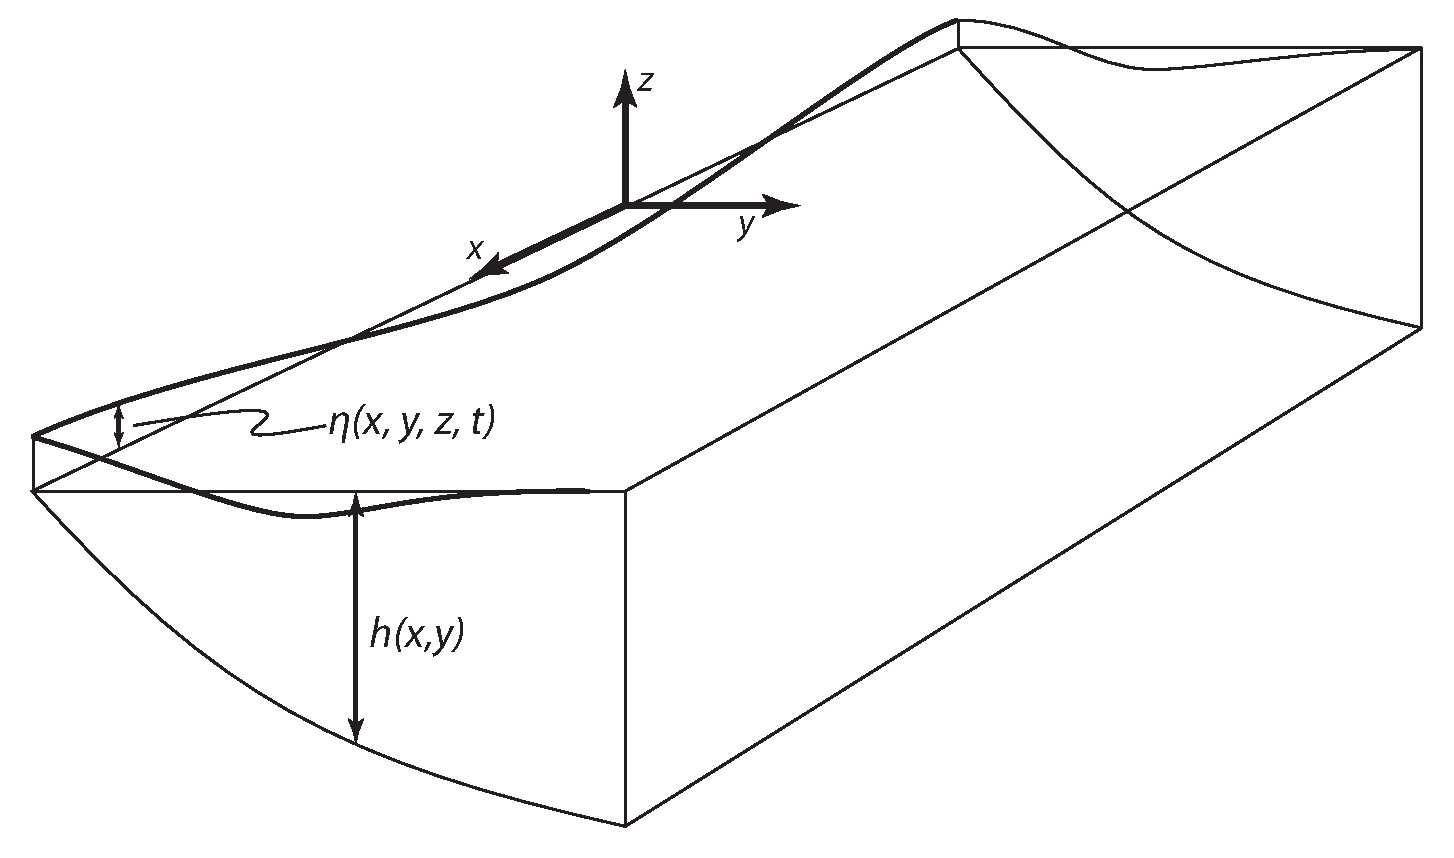
\includegraphics[width=5in]{basic_coastal_domain}   
    \caption{The basic coastal domain shows the orientation of the coordinate system, and shows how depth, $h$, and sea level elevation, $\eta$, are defined.}
    \label{fig:basic_coastal_domain}
\end{figure}

\newpage

\section{The equations of motion} 

The dynamical equations of motion are based on the Euler-Lagrange equations, given by
\begin{align}
    \frac{Du}{Dt} - fv &= 
        -\frac{1}{\rho_0}\frac{\partial p}{\partial x} 
        + \frac{\partial}{\partial x}(\nu \frac{\partial u}{\partial x} )  
        + \frac{\partial}{\partial y}(\nu \frac{\partial u}{\partial y} )  
        + \frac{\partial}{\partial z}(\nu \frac{\partial u}{\partial z} ) \label{eq:u-full} \\
    \frac{Dv}{Dt} + fu &= 
        -\frac{1}{\rho_0}\frac{\partial p}{\partial y} 
        + \frac{\partial}{\partial x}(\nu \frac{\partial v}{\partial x} )  
        + \frac{\partial}{\partial y}(\nu \frac{\partial v}{\partial y} )  
        + \frac{\partial}{\partial z}(\nu \frac{\partial v}{\partial z} ) \label{eq:v-full} \\
    \frac{Dw}{Dt}      &= 
        -\frac{1}{\rho_0}\frac{\partial p}{\partial z} - \frac{\rho g}{\rho_0} 
        + \frac{\partial}{\partial x}(\nu \frac{\partial w}{\partial x} )  
        + \frac{\partial}{\partial y}(\nu \frac{\partial w}{\partial y} )  
        + \frac{\partial}{\partial z}(\nu \frac{\partial w}{\partial z} ) \label{eq:w}\\
    \frac{\partial u}{\partial x} + \frac{\partial v}{\partial y} + \frac{\partial w}{\partial z} &= 0 \label{eq:cont}\\
    \frac{DS}{Dt} &= 
          \frac{\partial}{\partial x}(\nu_S \frac{\partial S}{\partial x} )  
        + \frac{\partial}{\partial y}(\nu_S \frac{\partial S}{\partial y} )  
        + \frac{\partial}{\partial z}(\nu_S \frac{\partial S}{\partial z} ) \label{eq:salt}\\
    \frac{DT}{Dt} &= 
          \frac{\partial}{\partial x}(\nu_T \frac{\partial T}{\partial x} )  
        + \frac{\partial}{\partial y}(\nu_T \frac{\partial T}{\partial y} )  
        + \frac{\partial}{\partial z}(\nu_T \frac{\partial T}{\partial z} ) \label{eq:temp}\\
    \rho &= \mathrm{EOS}(S, T, p) \label{eq:eos}
\end{align}
where EOS is an empirical {\it equation of state} relating temperature, salinity and pressure to density.  The total derivative is defines as
\begin{equation}
    \frac{D}{Dt} = \frac{\partial}{\partial t} + u \frac{\partial}{\partial x} 
                    + v \frac{\partial}{\partial y} + w \frac{\partial}{\partial z}.
\end{equation}
The molecular viscosity, $\nu$, and the molecular diffusivity of salt, $\nu_S$, and heat, $\nu_T$, may be considered to be approximately constant.  These molecular values are often replaced with turbulent viscosities and diffusivity, which may be orders of magnitude larger, and heterogeneous.  To calculate the turbulent viscosity or diffusivity from mean flow properties requires a {\it turbulence closure model}.  However, a down-gradient assumption is typically maintained, such that the equations maintain the same form, though the viscosities and diffusivities may no longer be assumed to be even approximately constant.

% sources and sinks in the T and S equations.

Equations~\ref{eq:u-full} through~\ref{eq:temp} are formally derived by considering a control volume, typically a cube, and relating the changes of properties within the cube to fluxes through the faces of the cube.  While important, this kind of derivation may be found in many other textbooks, and we will take a more heuristic approach here, and examine the character of the various terms in these equations.

\section{Eulerian vs. Lagrangian flow} 

Eulerian and Lagrangian flow describes two different ways to consider flow.  {\it Eulerian} flow considers properties at a fixed point in space, \emph{e.g.}, $u(x, y, z, t)$. {\it Lagrangian} flow, on the other hand, considers changes to a fixed parcel of water, following that parcel as it is moved by the flow field, \emph{e.g.}, $u(\mathrm{parcel~index}, t)$.  We almost always derive our equations using an Eulerian framework, as a Lagrangian framework requires a way to tag every parcel with a unique identifier.  Also, we often measure flow in an Eulerian framework, for example, moored current observations;  numerical models also output Eulerian flow.  In certain instances, however, when following a particular flow feature for example, the Lagrangian framework has clear advantages, but to obtain general solutions at all locations requires an infrastructure of identification tags that is too complex to do analytically.  Also, plankton and sediment particles move with the surrounding water, and experience the Lagrangian flow field.

Time derivatives in a Lagrangian framework are given by the {\it total derivative}, $D/Dt$, in the Eulerian framework by the partial derivative, $\partial/\partial t$.  These two views of the flow may be related by considering the chain rule,
\begin{equation}
  \label{eq:eulerian_vs_lagrangian}
  \begin{split}
    \frac{D}{Dt}\,u(x(t), y(t), z(t), t) &= \frac{\partial}{\partial t} 
                    + \frac{\partial x}{\partial t} \frac{\partial u}{\partial x} 
                    + \frac{\partial y}{\partial t} \frac{\partial u}{\partial y} 
                    + \frac{\partial z}{\partial t} \frac{\partial u}{\partial z} \\
                     &= \frac{\partial u}{\partial t} 
                    + u \frac{\partial u}{\partial x} 
                    + v \frac{\partial u}{\partial y} 
                    + w \frac{\partial u}{\partial z}
  \end{split}
\end{equation}
In the left side of this equation, in the Lagrangian framework, $x$, $y$, and $z$ are dependent variables that change in time, and represent the position of a particular water parcel.  On the right side, in the Eulerian framework, $x$, $y$, and $z$ are independent variables (not explicitly shown) and the derivatives with respect to the coordinate system must be converted to velocities, \emph{e.g.}, $u = \partial x/\partial t$.  

It should be noted that $u$ in equation~\ref{eq:eulerian_vs_lagrangian} may be replaced by any property of the flow, for example, any of the velocity components, temperature, salinity, or density.  If $D\phi/Dt=0$, that means that the property $\phi$ is {\it conserved}; that property will not change its value following a particular water parcel.  

\section{The advective terms} 
\label{sec:adv}

There are the three additional, non-linear terms that arise in equation~\ref{eq:eulerian_vs_lagrangian} in the Eulerian framework.  These three {\it advective} terms are at the root of the {\it closure} problem, the reason that time-mean variables cannot be substituted in the equations of motion, equations~\ref{eq:u-full} through~\ref{eq:temp}, while retaining the same mathematical structure; averaging these equations over some time interval causes new terms to arise.  To see this, let us define a time-averaging operator
\begin{equation}
    \langle\cdot\rangle = \frac{1}{T} \int^{T/2}_{-T/2} \cdot\;\;dt.
\end{equation}
Such an operation, applied to the momentum equations, is referred to as {\it Reynolds averaging}.  It is clear from this definition that the operator is linear, and has the following properties
\begin{equation}
    \langle c \phi\rangle = c \langle\phi\rangle, \quad \langle\langle\phi\rangle\rangle = \langle\phi\rangle, \quad \left\langle\frac{\partial \phi}{\partial t}\right\rangle = \frac{\partial}{\partial t}\langle\phi\rangle,
\end{equation}
where $\phi$ is some space- and time-dependent property of the flow, and $c$ is a constant.  These properties can be easily verified by reverting to the integral definition of the averaging operator, $\langle\cdot\rangle$. Of course, the time derivative in the third relation could be replaced with a derivative with respect to any other independent variable.  

Using this definition to average all of the terms in equations~\ref{eq:u-full} through~\ref{eq:temp} is straightforward for all the terms that are linear, where, for example, the pressure gradient, $p_x$, is simply replaced with the gradient of the time-averaged pressure, $\langle p \range_x$.  The advective terms\footnote{Typically the {\it molecular} diffusivity and viscosity terms are defined as, \emph{e.g.}, $\mu \partial^2 u/\partial z^2$; second order terms, but linear, as the molecular diffusivity or viscosity is generally treated as constant}, on the other hand, are non-linear, and so averaging these terms is not straightforward.  This is because, generally
\begin{equation}
    \langle\phi\,\psi\rangle \ne \langle\phi\rangle\langle\psi\rangle,
\end{equation}
and this is the form that the non-linear terms take; \emph{e.g.}, $\phi=u$, $\psi=\partial v/\partial x$.  The time mean of a product of two fluctuating terms is not equal to the product of the mean of the two terms because there may be correlations in the fluctuations of $\phi$ and $\psi$.  Do demonstrate this, consider the case when both $\phi$ and $\psi$ are periodic, and that the averaging interval is exactly one period.  In this case, obviously, $\langle\psi\rangle=0$ and $\langle\psi\rangle=0$.  However, if they are in phase, say, $\phi=\psi=\mathrm{sin}(2 \pi t / T)$, then, $\langle\phi \psi\rangle = T/2 \ne 0$.  These correlations are referred to as {\it eddy correlations}, and will be explored in much more detail in Chapter~\ref{chapter:turbulence} on Turbulence and Mixing.

It is possible for a flow that has zero mean in the Eulerian sense to still transport mass in the Lagrangian framework, even at scales much larger than turbulence.  For surface gravity waves, this phenomenon is referred to as {\it Stokes drift}\index{Stokes drift}.  \citet{longuet-higgins:69} describes this phenomenon for the more general case of unsteady currents.  This additional {Stokes velocity} is a consequence of the non-linear advective terms that are ultimately responsible for differences in the Lagrangian and Eulerian flow fields.

\begin{figure}[tb]
    \centering
    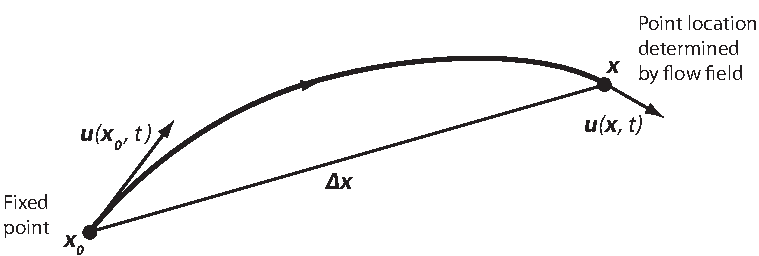
\includegraphics[width=5in]{stokes-diagram}   
    \caption{Diagram showing the variables used in the Stokes flow derivation.}
    \label{fig:stokes-diagram}
\end{figure}

Consider a flow vector, $\mathbf{u_0}$ at a fixed point $\mathbf{x_0}$.  Some small distance, $\mathbf{\Delta x}$, away at point $\mathbf{x}$, the flow is $\mathbf{u}$; see figure~\ref{fig:stokes-diagram}.  Now, let $\mathbf{\Delta x}$ be defined by an integral of the flow
\begin{equation}
    \mathbf{\Delta x} \simeq \int_{t_0}^{t} \mathbf{u_0} dx.
\end{equation}
Thus, we have the following relationship between $\mathbf u_0$ and $\mathbf u$
\begin{equation}
    \mathbf{u}(\mathbf{x}, t) = \mathbf{u_0}(\mathbf{x_0}, t) + \mathbf{\Delta x}\cdot\nabla\mathbf{u_0}
     = \mathbf{u_0}(\mathbf{x_0}, t) + \int_{t_0}^{t} \mathbf{u_0}\,dt\cdot\nabla\mathbf{u_0}.
\end{equation}
Note the similarities between this equation and equation~\ref{eq:eulerian_vs_lagrangian}, the dot product term is similar to the advective terms in the Eulerian definition of the total time derivative.  Now, time average this equation over one period of the process of interest (wave period, tidal period, \emph{etc.}), to get
\begin{equation}
    \langle \mathbf{u}(\mathbf{x}, t) \rangle
     = \langle \mathbf{u_0}(\mathbf{x_0}, t) \rangle 
     + \left\langle \int_{t_0}^{t} \mathbf{u_0}\,dt\cdot\nabla\mathbf{u_0} \right\rangle
\end{equation}
where $\langle\cdot\rangle$ is the time-averaging operator.  Since $\mathbf x_0$ defines a fixed point, the velocity here represents the Eulerian velocity.   But since the position of $\mathbf x$ is defined by the direction of the flow and the time $t$, this represents the Lagrangian velocity.  The rightmost term is then referred to as the {\it Stokes velocity}.  Thus, we can define the difference in the Lagrangian and Eulerian velocities is defined as the Stokes velocity,
\begin{equation}
    \langle \mathbf{u_{\mathrm{Lagrangian}}} \rangle = 
        \langle \mathbf{u_{\mathrm{Eulerian}}} \rangle + 
        \langle \mathbf{u_{\mathrm{Stokes}}} \rangle.
\end{equation}

Again, we see that the time mean of flow following a parcel has additional terms relative the the mean flow at a single point.  This, again, is due to correlations in the flow and the gradients of the flow.  For a periodic flow, the Stokes velocity will be largest when the flow and flow gradients are in phase.  

Consider a propagating wave traveling in the $x$-direction,
\begin{equation}
    u = U_0\,\mathrm{sin}(kx - \omega t)
\end{equation}
Clearly, the mean Eulerian velocity is zero.  Averaging over one period, the Stokes velocity (also the Lagrangian velocity), though, is
\begin{equation}
    \langle \mathbf{u_{\mathrm{Lagrangian}}} \rangle =
    \langle \mathbf{u_{\mathrm{Stokes}}} \rangle 
            = \left\langle \int_{t_0}^{t} \mathbf{u_0}\,dt\cdot\nabla\mathbf{u_0} \right\rangle 
            = \left\langle \frac{U_0^2\,k}{\omega} cos^2(kx - \omega t)  \right\rangle 
            = \frac{U_0^2}{2 c}
\end{equation}
where $c=\omega\,k^{-1}$ is the phase speed of the wave.

Now, consider a steady flow, but increasing in magnitude in the $x$-direction, such that
\begin{equation}
    u > 0\quad,\quad \frac{\partial u}{\partial x} > 0.
\end{equation}
Eulerian flow at some point, $x_0$, is simply $u(x_0)$.  However, if we follow a parcel released at point $x_0$ for some time, it will have a mean velocity greater than $u(x_0)$, because $u(x_0)$ will be the smallest velocity that the parcel experiences.  Thus, the correlations between the velocity and velocity gradients that cause the differences between Eulerian and Lagrangian flow do not necessarily need to be time dependent, although fluctuating currents are usually how we usually think about Stokes drift.

As this section demonstrates, the non-linear terms are an important aspect of the hydrodynamic equations.  These terms are responsible for the chaotic nature of flows at all scales.  One aspect of this is the nature of small-scale turbulent flows that may influence flow at larger scales.  Parameterization of turbulent flows in numerical models is necessary because numerical models of (primarily hydrostatic) geophysical flow do not come close to resolving even the largest eddies (for isotropic turbulence, where the aspect ratio of the turbulent eddies is approximately one and the flow is nonhydrostatic).  These turbulent eddies, that are generated by instabilities in larger scale flow, influence the larger scale motions through variations in turbulent viscosity and diffusivity in a way that is difficult to predict accurately.

Because it is difficult to solve chaotic, non-linear systems analytically, many of our conceptual models of geophysical flow are based on linear models, where the influence of the advective terms is assumed to be negligible.  These linear, analytical models of geophysical flow are useful, however, in that they increase our intuition about the character of geophysical scale flows.  It is difficult to gain an intuition for large-scale, rotating flows because the flows we experience directly (flow in a river, or a swimming pool, or a sink) are non-rotating, and rotating flows behave very differently from non-rotating flows.  That said, as suggested by the discussion above, we should be careful about placing too much faith in any solution that was derived ignoring the advective terms.

\section{Scales and non-dimensional numbers}

Ratios of the terms, expressed as non-dimensional numbers, in the equations of motion are used to justify exclusion of certain terms from the momentum balance.  Often, this is presented in the following manner:  the scales of the flow are stated, the various non-dimensional parameters are calculated using these values, and the small terms are identified and eliminated.  In practice, this procedure is done in reverse.  Given a set of basic analytical models, it is often clear how one would like to extend these models by adding certain terms.  Or, it is possible that intuition about the problem suggests that certain processes must be dominant, and others may be ignored.  Or, finally, a set of terms is chosen such that it is possible to derive a simple, analytical solution, and the situations where this solution is valid are determined after the fact.  In any case, it is a useful exercise to see if the appropriate non-dimensional parameters are indeed small, and the associated scales are consistent with the process under investigation.

As we are dealing with very simple, well-known solutions of basic balances in this book, we will state which terms will be kept and which will be ignored, and then state which non-dimensional numbers must be large or small to support this balance.  This will determine over which scales the simple solutions are valid.

The spatial scales are a depth scale, $H$, for the vertical scale, and $L$ for (isotropic) horizontal scales; $L_x$ and $L_y$ for along- and cross-shore scales when the scales are not isotropic.  Dependent variable scales are $U$ for the horizontal velocity scale, $\eta_0$ for the magnitude of sea surface displacements, and $\nu$ for viscosity.  Other dimensional scales of the system include the rotational timescale $f^{-1}$ (where $f$ is the Coriolis parameter), the gravity wave phase speed, $c=\sqrt{g\,H}$ (where $g$ is the gravitational acceleration), and the {\it deformation radius}, $R_d=\sqrt{g\,H}\,f^{-1}$, for the horizontal scale.  The deformation radius is the distance a gravity wave can travel in the timescale $f^{-1}$, and sets the dominant horizontal scale for rotating flow.  

The effects of stratification are measured by the {\it stratification frequency}, $N$, defined by
\begin{equation}
    N^2 = -\frac{g}{\rho_0}\frac{\partial \rho}{\partial z},
\end{equation}
which is the natural frequency of internal waves associated with motions of the density field of a continuously stratified fluid.  If the fluid has a sharp pycnocline separating two or more relatively homogeneous layers, a more relevant scale may be the {\it internal phase speed},
\begin{equation}
    c' = \sqrt{g'\,H} = \sqrt{\frac{g\,\Delta\rho\,H}{\rho_0}}
\end{equation}
where $\Delta\rho$ is the density difference across the pycnocline.  The {\it reduced-gravity}, $g'$, represents the weakened effect of gravity on fluids of nearly the same density; typical values of $\Delta\rho\,\rho_0^{-1}$ in natural geophysical systems are at most about 0.02, and often much less.  The internal phase speed may be used to define an {\it internal deformation radius}, $R_d'=\sqrt{g'\,H}\,f^{-1}$, which is the relevant horizontal length scale for a stratified flow with two layers.  

\paragraph{Reynolds number} \index{Reynolds number}
\begin{equation}
    Re = \frac{U\,L}{\nu}
\end{equation}
The Reynolds number is a ratio of the advective terms to the (molecular) viscosity terms.  Here $\nu$ is the {\it kinematic molecular viscosity}; for water $\nu\simeq10^{-6}$~m$^2$~s$^{-1}$.  The Reynolds number is usually used to characterize the tendency of a flow to be turbulent, larger Reynolds numbers indicate that the flow is more likely to be turbulent.  The exact value of the Reynolds number at which the transition to turbulent flow occurs depends on many of the details of the problem; \emph{e.g.}, flow through a pipe {\it vs.} flow over a plate.  The roughness of the boundaries and the details of the flow initiation also matter.  Generally, though we expect a transition to turbulence for $Re\sim\mathcal{O}$(10$^3$), fully developed turbulence for $Re\sim\mathcal{O}$(10$^5$).  The Reynolds number for geophysical flows are typically as large or larger than that required for fully developed turbulence, and so the Reynolds number is only used in the study of turbulence.  We assume that the flow in the ocean is always potentially turbulent.


\paragraph{Rossby number} \index{Rossby number}
\begin{equation}
    Ro = \frac{U}{f\,L}
\end{equation}
The Rossby number is a ratio of the advective terms to the Coriolis term.  It is a measure of the non-linearity or instability of the flow.  For the sake of creating a tractable problem, we often assume a small Rossby number, $Ro\ll\mathcal{O}(1)$, so that the advective terms may be neglected.  This assumption requires large horizontal spatial scales and long timescales to be valid.  While this assumption is very useful, and can produce analytical models with reasonable predictive ability, any assumption that neglects the advective terms is best initially met with a healthy skepticism.

\paragraph{Ekman number} \index{Ekman number}
\begin{equation}
    Ek = \frac{\kappa}{f\,H^2}
\end{equation}
The Ekman number is a ratio between the viscous terms and the Coriolis term.  Here, $\kappa$ is the {\it turbulent kinematic eddy viscosity}, the effective eddy viscosity that a fluid feels when the flow properties are averaged over timescales much longer than the timescale of turbulent eddy overturns.  The turbulent viscosity is typically a few orders of magnitude larger than the molecular viscosity.  If the Ekman number is small, $Ek\ll\mathcal{O}(1)$, rotational effects are more important than viscous effects, and the flow may be considered to be inviscid.  Unlike non-rotational flows, rotation limits the distance that a boundary stress may penetrate into a fluid.  The thickness of the boundary layers where viscous effects are important is called the {\it Ekman depth}, $\delta$, and may be estimated by setting $Ek=1$, and solving for the vertical length scale,
\begin{equation}
    \delta = \sqrt{\frac{f}{\kappa}}.
\end{equation}
The Ekman depth may be reduced by the presence of stratification, which inhibits turbulence and reduces $\kappa$.  Typical scales for the Ekman depth are a few meters, so that the interior of the ocean, away from the boundaries, the flow may be considered to be inviscid.

\paragraph{Richardson number} \index{Richardson number}
\begin{equation}
    Ri = \frac{N^2}{S^2} \simeq \frac{g'\,H}{U^2}
\end{equation}
where $S^2 = (u_{zz})^2$ is the shear squared.  These two definitions are termed the {\it gradient Richardson number} and the {\it bulk Richardson number}, respectively.  The Richardson number may be considered a ratio of the potential energy inherent in the stratification ($N^2$) to the kinetic energy inherent in the velocity shear ($S^2$).  The critical value for the gradient Richardson number is approximately 0.25 (we will derive this fact later), and slightly larger (but certainly less than one) for the bulk Richardson number.  When the Richardson number is smaller than the critical value, the shear in the flow is able to overcome the potential energy barrier associated with the stratification, and the fluid will mix.  When the Richardson number is larger than the critical value, the shear is unable to overcome the stratification, and the fluid is stable, mixing is inhibited.  There are other definitions of the Richardson and Froude numbers that are specific to characterizations of turbulent flow; these will not introduce here, but will be saved for the chapter on turbulent flows.

\paragraph{Internal Froude number} \index{Froude number!Internal}
\begin{equation}
    Fr = \frac{U}{\sqrt{g'\,H}}
\end{equation}
The Froude number is a ratio of the flow speed to the internal gravity wave speed.  Here, we have defined the {\it internal} or {\it baroclinic} Froude number, associated with internal, density waves.  We could also define a {\it barotropic} Froude number, but for geophysical flows, this number is always much, much less than one, and it is consequently of less use in characterizing flows.  The nature of the flow changes when the Froude number exceeds one, since then gravity waves travel slower than the flow speed and are unable to propagate upstream.  Froude numbers greater than one are associated with {\it supercritical flow}.  Typically, the internal Froude number over the shelf is much less than one.  The Froude number may approach or slightly exceed one in estuaries, river plumes, and frontal regions.  Froude numbers greater than two are rare.  Note that the Richardson number and Froude number are related, $Ri = Fr^{-2}$.  Despite the fact that no new information is contained in having two separate numbers, they are traditionally used to discuss very different processes.  The Froude number is used to characterize hydraulic control and other advective processes, the Richardson number is used to characterize mixing processes.


\paragraph{Burger number} \index{Burger number}
\begin{equation}
    Bu = \frac{N\,H}{f\,L} = \alpha\frac{N}{f}
\end{equation}
The Burger number relates the importance of stratification to rotation; for small values of the Burger number, rotational effects are more important than stratification.  Sometimes the square of the right hand side is used to define the Burger number.  The bathymetric slope, $\alpha = h_x \simeq H\,L^{-1}$, may be used to define the {\it slope Burger number}, far right.

\paragraph{Kelvin number} \index{Kelvin number}
\begin{equation}
    K = \frac{L\,f}{\sqrt{g'\,H}}
\end{equation}
The Kelvin number is used to relate the length scale of a feature, say the width of an estuary mouth, to the deformation radius.  Notice that if we approximate $N\,H = \sqrt{g'\,H}$, the Kelvin and Burger numbers are related by $K=Bu^{-1}$.

There are many other non-dimensional numbers, but this list will be sufficient for nearly all of the cases that we deal with in this book.


%%%%%%%%%%%%%%%%%%%%%%%%%%%%%%%%%%%%%%%%%%%%%%%%%%%%%%%%%%%%%%%%%%%%%%%%%%%%%%
%%%%%%%%%%%%%%%  BAROTROPIC FLOW CHAPTER  %%%%%%%%%%%%%%%%%%%%%%%%%%%%%%%%%%%%
%%%%%%%%%%%%%%%%%%%%%%%%%%%%%%%%%%%%%%%%%%%%%%%%%%%%%%%%%%%%%%%%%%%%%%%%%%%%%%

\chapter{Barotropic flow}

In this chapter, we consider simple problems in which density differences in the ocean are ignored.  In this case, the pressure gradient in the fluid is determined solely by gradients in the sea surface.  Such flow conditions also arise when the flow contains density gradients.  For stratified flow there can be many modes of variability, and the gravest mode is typically similar to barotropic flow.  As such, this type of flow is often referred to as the {\it external} mode, related to changes in the sea surface, where the {internal} modes are associated with changes in the density field within the fluid.

Consider a homogeneous, inviscid fluid -- let us assume for the moment, without a formal scaling analysis, that these are both reasonable assumptions.  In this case, since $S$, $T$, and $\rho$ are all constant (with $\rho=\rho_0$), the only non-trivial equations from~\ref{eq:u-full} to~\ref{eq:eos} are the first four, which are now,
\begin{align}
    \frac{\partial u}{\partial t} 
        + u\frac{\partial u}{\partial x} 
        + v\frac{\partial u}{\partial y} 
        + w\frac{\partial u}{\partial z} - fv 
                &= -\frac{1}{\rho_0}\frac{\partial p}{\partial x} \label{eq:u-barotropic} \\
    \frac{\partial v}{\partial t} 
        + u\frac{\partial v}{\partial x} 
        + v\frac{\partial v}{\partial y} 
        + w\frac{\partial v}{\partial z} + fu 
                &= -\frac{1}{\rho_0}\frac{\partial p}{\partial y}  \label{eq:v-barotropic} \\
    \frac{\partial w}{\partial t}  
        + u\frac{\partial w}{\partial x} 
        + v\frac{\partial w}{\partial y} 
        + w\frac{\partial w}{\partial z}
                &= -\frac{1}{\rho_0}\frac{\partial p}{\partial z} - g \label{eq:w-barotropic}\\
    \frac{\partial u}{\partial x} 
        + \frac{\partial v}{\partial y} 
        + \frac{\partial w}{\partial z} 
                &= 0 \label{eq:cont-barotropic}
\end{align}
There are four equations, and four dependent state variables: $u$, $v$, $w$, and $p$.  We will proceed to reduce this set of four equations to a set of three equations in $u$, $v$, and $\eta$.  This is possible because the hydrostatic assumption trivializes the vertical momentum equation.

\section{The hydrostatic balance}

The dominant balance in the vertical momentum equation (equation~\ref{eq:w-barotropic}) is between the vertical pressure gradient and gravity.  Essentially, this means that the pressure at any point in the fluid is equal to the weight of the water above it, and is not influenced by the local flow field\footnote{\emph{hydro} means water, \emph{static} means not moving, so the hydrostatic balance is the balance the flow would have at rest.}  The terms in the vertical momentum equation can be scaled in order to quantify this.  Horizontal distances, $x$ and $y$, and velocities, $u$ and $v$, will be scaled as $L$ and $U$, respectively; the vertical coordinate, $z$, and velocity, $w$, will be scaled as $H$ and $W$, respectively.  The timescale, $T$, may be related to the flow by the relationship $T=L\,U^{-1}=H\,W^{-1}$, \emph{e.g.}, the time it takes a parcel with a velocity $U$ to flow a distance $L$.  Derivatives are scaled as, for example, $u\,u_x = U^2 L^{-1}$ (subscripts denote partial differentiation).

Note that, by scaling the continuity equation (equation~\ref{eq:cont-barotropic}),
\begin{equation}
    \frac{U}{L} = \frac{W}{H}.
\end{equation}
This equation along with the timescale relationship can be used to show all the terms on the left hand side of equation~\ref{eq:w-barotropic} have the same magnitude,
\begin{equation}
    \frac{W}{T} = \frac{U\,W}{L} = \frac{W^2}{H}.
\end{equation}

At this point, it is unclear how to scale the pressure, we may assume it will be as large as needed to balance the equation. Now, if we compare the advective terms in the vertical momentum equation to gravity, $g$, we obtain
\begin{equation}
    \frac{\mathrm{Advective~term}}{\mathrm{Gravity}} = \frac{U\,W}{g\,L} = \frac{U^2}{g\,H}\frac{H^2}{L^2} = Fr^2 \alpha^2 
\end{equation}
where $Fr=U (g\,H)^{-1/2}$ is the Froude number, a ratio of the flow speed to the gravity wave speed, and $\alpha=H\,L^{-1}$ is the aspect ratio of the flow.  Note that, if we allowed for variations in density, we could simpily substitute the internal Froude number for the Froude number.  Typically, for geophysical scale flows, the Froude number is very small, and even the internal Froude number is never larger than about 2.  The aspect ratio, $\alpha$, is always very small, typically around 10$^{-2}$ to 10$^{-4}$.  For example, typical scales might include an estuary that is 10~m deep with cross-channel scales of about a kilometer ($\alpha$=10$^-2$) and along-channel scales of about 10~km ($\alpha$=10$^-3$), or a continental shelf with a depth of 100~m and horizontal scales of 10~km ($\alpha$=10$^-3$) or 100~km ($\alpha$=10$^-4$).  Thus, even given a very large Froude number of $\mathcal{O}(1)$, and a very large aspect ratio of 0.1, the advective terms will only be about one percent of the total balance.  Thus, the dominant balance is between gravity and the pressure gradient.  Non-hydrostatic flows must be both energetic and isotropic, like turbulence; the assumption of a hydrostatic balance is extremely reasonable and accurate for all of the other flow regimes we will consider here.

Because the pressure never appears explicitly in the momentum equations -- only pressure gradients -- we may subtract out the mean gradient from the hydrostatic balance, to define the perturbation pressure
\begin{equation}
    \label{eq:pprime}
    p' = p - p_{\mathrm{hydrostatic}},
\end{equation}
where the hydrostatic pressure is defined as
\begin{equation}
    p_{\mathrm{hydrostatic}} = \rho_0\,g\,z,
\end{equation}
the pressure due to the weight of the water column at some depth $z$, referenced to $p_{\mathrm{hydrostatic}}=0$ at the geopotential $z=0$.  The gradient of equation~\ref{eq:pprime} with respect to $z$, and substitution into the remaining terms of equation~\ref{eq:w-barotropic} gives
\begin{equation}
    \label{eq:hydrostatic}
    \frac{\partial p'}{\partial z} = 0.
\end{equation}
Note that by the definition of $p'$ in equation~\ref{eq:pprime},
\begin{equation}
    \frac{\partial p'}{\partial x} = \frac{\partial p}{\partial x} \quad , \quad
    \frac{\partial p'}{\partial y} = \frac{\partial p}{\partial y}.
\end{equation}
so that equation~\ref{eq:hydrostatic} can replace the vertical momentum equation (equation~\ref{eq:w-barotropic}) in the equations of motion, and $p'$ may replace $p$ in equations~\ref{eq:u-barotropic} and~\ref{eq:v-barotropic}.  Both pressure, $p$, and perturbation pressure, $p'$, are used in this book and in the literature; the presence of a gravity term in the vertical momentum equation will determine which is being used.

\section{The inviscid shallow water equations}

Because the hydrostatic balance states there is no vertical pressure gradient, there will be no vertical shear that develops in the horizontal currents, or
\begin{equation}
    \frac{\partial u}{\partial z} = \frac{\partial v}{\partial z} = 0,
\end{equation}
if there are no such gradients initially.  This is because if there is no vertical shear initially, none of the terms in equations~\ref{eq:u-barotropic} and~\ref{eq:v-barotropic} will generate such a shear.  Move all the terms except the time derivative to the right hand side -- none of the terms now on the left depend on vertical gradients (except, the $w\,u_z$ and $w\,v_z$ terms, which are both assumed to be zero initially).   If the right hand side does not depend on $z$ initially, there is no way for vertical gradients to form.  In other words, there is no source for lateral vorticity.  Viscosity and stratification can both break this balance, and generate vertical shear.

The lack of vertical shear implies that the vertical velocity may be determined diagnostically from the horizontal flow field and the surface and bottom boundary conditions, reducing the number of dependent variables and degrees of freedom by one.  In order to do this, we will vertically integrate the horizontal momentum equations from the sea floor, $z=-h$, to the sea surface, $z=\eta$.  Both of these are material surfaces that water cannot flow through.  This is defined mathematically as
\begin{align}
    \frac{D h}{Dt} &= u \frac{\partial h}{\partial x} + v \frac{\partial h}{\partial y} = -w|_{z=-h} \label{eq:h_cons}, \\
    \frac{D \eta}{Dt} &= \frac{\partial \eta}{\partial t} + u \frac{\partial \eta}{\partial x} + v \frac{\partial \eta}{\partial y} = w|_{z=\eta}. \label{eq:eta_cons}
\end{align}
These total derivatives define the vertical velocity of a parcel on the material surface.  Note that a parcel on the material surface remains forever on that surface; since there is no vertical shear, there is no mechanism to separate the parcel from the surface.  Also note, the material surface does not need to move in order for there to be a vertical velocity there; flow along a bathymetric gradient will produce a vertical velocity (\emph{e.g.}, $u\,h_x$) even with the bathymetry is stationary.

Because there is no vertical shear in the flow, all of the terms in equations~\ref{eq:u-barotropic} and~\ref{eq:v-barotropic} are independent of depth.  A vertical average then just gives those identical equations.  A vertical integral of the continuity equation, on the other hand, requires a bit more care, because while the shear in the lateral currents is zero, the vertical velocity is not necessarily zero and is not necessarily uniform with depth.  For example, a vertical velocity may be generated, as we have just shown, by flow along bathymetric gradients, and the surface and bottom vertical velocities may be different.  So, a vertical integral of the continuity equation (equation~\ref{eq:cont-barotropic}) over the range $z=(-h, \eta)$ results in the following relation
\begin{equation}
    (h+\eta)\frac{\partial u}{\partial x} + (h+\eta)\frac{\partial v}{\partial y} + w|_{z=\eta} - w|_{z=-h} = 0.
\end{equation}
Here, we have made use of the fact that the lateral velocities are depth dependent, and thus so is the lateral shear of the lateral velocities.  If there we consider the case with vertical shear, a similar relation can be derived, but Leibniz integral rule for variable integration limits\footnote{See, {\tt http://en.wikipedia.org/wiki/Leibniz\_integral\_rule} or \citet{kundu:90}, page 75.}  must be used.  The final result is identical, but with the horizontal velocities replaced with depth mean values. Substitution of the definitions for velocity on a material surface gives
\begin{equation}
    (h+\eta)\frac{\partial u}{\partial x} + (h+\eta)\frac{\partial v}{\partial y} + \frac{\partial \eta}{\partial t} + u \frac{\partial \eta}{\partial x} + v \frac{\partial \eta}{\partial y} + u \frac{\partial h}{\partial x} + v \frac{\partial h}{\partial y} = 0.
\end{equation}
This equation may be simplified by combining like terms, and assuming $\eta \ll h$, a reasonable assumption in all but very near-shore regions, where $h$ is small, or regions with an exceptionally large tidal range, where $\eta$ is large.  Typically subtidal variations in $\eta$ are $\mathcal{O}$(0.1~m), where typical depth ranges we are concerned with here are $\mathcal{O}$(10-100~m).  Thus, $h+\eta \simeq h$ is usually a reasonable approximation.  The new, simplified continuity equation is
\begin{equation}
    \frac{\partial}{\partial x}(u h) + \frac{\partial}{\partial y}(v h) + \frac{\partial \eta}{\partial t} = 0. \label{eq:cont-shallow-placeholder}
\end{equation}
In other words, convergence in horizontal transport causes sea level to rise, and {\it vice verse}.

The final step in our derivation of the shallow water equations is to rewrite the horizontal pressure gradients in terms of sea level variations.  This is done by integrating the hydrostatic pressure gradient from some reference level within the water up to the sea surface, $z=(z_0, \eta)$.  Here, we need the gradient of the actual pressure, not the perturbation pressure, as we need to calculate the pressure changes caused by the weight of the water in the sea level anomaly, so
\begin{equation}
    \int_{z_0}^\eta \frac{\partial p}{\partial z} \,dz = \int_{z_0}^\eta \rho_0\,g\,dz.
\end{equation}
Both integrals are trivial to calculate,
\begin{equation}
    p|_{z=z_0} = p_{ATM} + (\eta-z_0)\rho_0\,g.
\end{equation}
The pressure at the surface is defined to be the atmospheric pressure, $p_{ATM}$ which we will assume for simplicity has no horizontal gradients. This assumption may be relaxed, but the ocean typically responds to differences in atmospheric pressure by adjusting sea level to cancel these pressure differences out, referred to as the {\it inverse barometer effect}.  We are interested in finding the horizontal pressure gradients at $z=z_0$.  A derivative with respect to $x$, for example, after some minor rearrangement, is
\begin{equation}
    \frac{1}{\rho_0}\frac{\partial p}{\partial x} = g\frac{\partial \eta}{\partial x}.
\end{equation}
The gradient with respect to $y$ is similar.

Now, we have all the components to rewrite equations~\ref{eq:u-barotropic} through~\ref{eq:cont-barotropic} as a system of three equations in $u$, $v$, and $\eta$
\begin{align}
    \frac{\partial u}{\partial t} 
        + u\frac{\partial u}{\partial x} 
        + v\frac{\partial u}{\partial y} - fv 
                &= -g\frac{\partial \eta}{\partial x} \label{eq:u-shallow} \\
    \frac{\partial v}{\partial t} 
        + u\frac{\partial v}{\partial x} 
        + v\frac{\partial v}{\partial y} + fu 
                &= -g\frac{\partial \eta}{\partial y}  \label{eq:v-shallow} \\
    \frac{\partial}{\partial x} (u\,h)
        + \frac{\partial }{\partial y} (v\,h)
        + \frac{\partial \eta}{\partial t} 
                &= 0. \label{eq:cont-shallow}
\end{align}

%%%% Note on d eta / dt term being as small as the others ignored.

\section{Geostrophic flow}\index{Geostrophy}\index{Geostrophic flow}

Geophysical flows are characterized by large spatial scales and long timescales.  It may be demonstrated through a scaling analysis that subinertial flow, defined as flow with timescales longer than $f^{-1}$, on the continental shelf is very nearly in geostrophic balance, with the pressure gradient term balancing the Coriolis term.  This requires that frictional effects are weak ($Ek\ll1$), and that the Rossby number is small.  In this case, the flow is quasi-steady, and the dominant balance is given by the equations
\begin{align}
     - fv 
                &= -g\frac{\partial \eta}{\partial x} \label{eq:u-geostrophic} \\
    fu 
                &= -g\frac{\partial \eta}{\partial y}  \label{eq:v-geostrophic} \\
    \frac{\partial}{\partial x} (u\,h)
        + \frac{\partial }{\partial y} (v\,h)
                &= 0 . \label{eq:cont-steady}
\end{align}
For the case of constant depth, $h(x, y)=H$, this system of equation is degenerate, in that the {\it geostrophic flow} specified by the momentum equations (equations~\ref{eq:u-geostrophic} and~\ref{eq:v-geostrophic}) automatically satisfies the continuity equation (equation~\ref{eq:cont-steady}).  This can be seen by taking the {\it curl of the equations}: an $x$-derivative of equation~\ref{eq:v-geostrophic} subtracted by a $y$-derivative of equation~\ref{eq:u-geostrophic} shows that the flow is non-divergent, $u_x + v_y = 0$.  Thus, the continuity equation provides no new information, and we are left with three variables, but only two independent equations to define them; any horizontally non-divergent flow automatically satisfies geostrophy.

For variable topography, the combination of no divergence in the flow (from geostrophy), and no divergence in the transport (from continuity) requires that the flow must follow constant depth contours.  This can be seen explicitly by substituting u in equations~\ref{eq:u-geostrophic} and~\ref{eq:v-geostrophic} into the continuity equation (this is a technique we will use often), to get
\begin{equation}
    - \frac{g}{f}\frac{\partial}{\partial x} (\frac{\partial \eta}{\partial y}\,h) 
        + \frac{g}{f}\frac{\partial }{\partial y} (\frac{\partial \eta}{\partial x}\,h)
    = - \frac{\partial \eta}{\partial y}\frac{\partial h}{\partial x}
        + \frac{\partial \eta}{\partial x}\frac{\partial h}{\partial y}
    \equiv J(\eta, h) = 0,
\end{equation}
where $J(\eta, h)$ is the Jacobean of $h$ and $\eta$.  If the Jacobean of two variables equals zero, it means that one may be written as a function of the other, \emph{i.e.}, $\eta=\eta(h)$.  This may be demonstrated by substituting this relationship into the definition of the Jacobean, and using the chain rule
\begin{equation}
    J(\eta(h), h) = 
          \frac{\partial \eta}{\partial x}\frac{\partial h}{\partial y} 
        - \frac{\partial \eta}{\partial y}\frac{\partial h}{\partial x} = 
        = \frac{\partial \eta}{\partial h}\frac{\partial h}{\partial x}\frac{\partial h}{\partial y} 
        - \frac{\partial \eta}{\partial h}\frac{\partial h}{\partial y}\frac{\partial h}{\partial x} = 0.
\end{equation}
If $\eta$ is a function of $h$, this implies that the contours of both of these must overlap, \emph{i.e.}, if $h=\mathrm{contant}$, then $\eta=\mathrm{constant}$ must be so as well.

Geostrophic flow follows contours of $\eta$.  This may be demonstrated by using geometric arguments to define a streamfunction, $\psi$.  If we define the streamfunction as
\begin{align}
    \frac{\partial \psi}{\partial x} &= v \\
    \frac{\partial \psi}{\partial y} &= - u
\end{align}
substitution into equation~\ref{eq:cont-steady} shows that this definition of the streamfunction automatically satisfies the continuity equation.  Note that comparison of the streamfunction definition with equations~\ref{eq:u-geostrophic} and~\ref{eq:v-geostrophic} shows that $\eta$ and $\psi$ differ only by a constant, $g f^{-1}$, thus, contours of constant $\eta$ and constant $\psi$ overlap.  A geometric argument showing that the flow follows constant values of the streamfunction is shown in figure~\ref{fig:streamfunction}

\begin{figure}[tb]
    \centering
    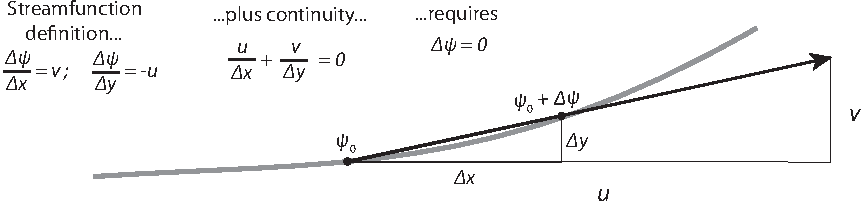
\includegraphics[width=6in]{streamfunction}   
    \caption{A geometric argument showing that flow follows constant values of the streamfunction, $\psi$.}
    \label{fig:streamfunction}
\end{figure}

The flow is thus required to follow constant values of $\eta$, $\psi$, and $h$.  The inability of the flow to cross bathymetric contours means that the flow may never change its thickness.  In other words, columns of water are ridged, and may never be compressed or stretched.  This is similar to the result derived in the previous section, that there is no vertical shear in the horizontal currents for frictionless flow.  However, in the previous case, it was possible for flow to cross isobaths; as non-rotating flow enters shallow water, it will accelerate by continuity.  Geostrophic flow, on the other hand, is unable to cross isobaths.  However, geostrophic flow is still able to accelerate or decelerate according to the bathymetric gradients; as depth contours converge, the transport between these contours must remain constant, so the flow accelerate to maintain the same transport through a narrower cross-section.  Flow on closed bathymetric contours, for example a seamount, will be isolated from the surrounding flow.  This effect is often referred to as a \emph{Taylor column}\index{Taylor column}, where the vertical rigidity of geostrophic flow prevents onto or off of a localized shallow region.

Large-scale flow in the coastal ocean is very nearly geostrophic.  However, as we have seen above, the equations are degenerate -- the geostrophic momentum equations automatically satisfy the continuity equation.  Thus, actual solutions must be sought by examining the balance in smaller terms.  While it is clear that geostrophy is the dominant, first-order balance for large-scale shelf circulation, there is not one single clear choice for what the second-order balance should be in all circumstances.  For smaller scale processes, geostrophy looses its preeminence;  it is common for flow very near shore or within an estuary to have a dominant balance that is not geostrophic.

\section{Potential vorticity}\index{Potential vorticity}

Conservation of potential vorticity is one of the most powerful concepts in geophysical fluid dynamics.  For the shallow water equations, we will derive this for the linear shallow water equations, where the advective terms are excluded, but the time derivative terms are retained; this requires low Rossby number flow conditions.  We will also, for now, consider a domain with constant depth, $h=H$.  The starting point is then
\begin{align}
    \frac{\partial u}{\partial t} - f v
                &= -g\frac{\partial \eta}{\partial x} \label{eq:u-shallow-linear} \\
    \frac{\partial v}{\partial t} + f u
                &= -g\frac{\partial \eta}{\partial y}  \label{eq:v-shallow-linear} \\
    H\left(\frac{\partial u}{\partial x} + \frac{\partial v}{\partial y}\right)
        + \frac{\partial \eta}{\partial t} 
                &= 0. \label{eq:cont-shallow-linear}
\end{align}
To proceed, we will first take the curl of the momentum equations, and add them together.  Notice, here, the pressure gradient terms cancel,
\begin{equation}
    v_{xt} + f u_x - u{yt} + f v_y = \zeta_t - \frac{f}{H}\eta_t = 0
\end{equation}
where $\zeta = v_x - u_y$ is the curl of the velocity, and the continuity equation has been used to exchange the flow divergence for the time derivative of sea surface height.  This is a statement of {\it conservation of potential vorticity}, or
\begin{equation}
    \frac{\partial}{\partial t}\left(\frac{\zeta}{f} - \frac{\eta}{H} \right) = 0.
    \label{eq:linear-pv-conservation}
\end{equation}
A more general form of potential vorticity conservation may be derived from the shallow water equations, including the advective terms and variations in bathymetry, as
\begin{equation}
    \frac{D}{Dt} \left( \frac{f + \zeta}{h} \right) = 0 .
    \label{eq:pv-conservation}
\end{equation}
This requires a more lengthy derivation, and it is sometimes easier to work both backwards from the final statement and forwards from the shallow water equations to prove this.  

Consider quiescent flow in a region with constant bathymetric gradients, $h = H + h_y \Delta y$.  The potential vorticity is then, assuming that $h_y\,\Delta y\,H^{-1} \ll 1$, approximately
\begin{equation}
    \frac{f}{H} \left( \frac{1}{1 + h_y\,\Delta y\,H^{-1}} \right)
        \sim \frac{f}{H}\left(1 - \frac{h_y\,\Delta y}{H}\right)
        = \frac{f - f\,h_y\,H^{-1}\,\Delta y }{H}.
\end{equation}
Here, it is clear that $f h_y H^{-1}$ acts as a potential vorticity gradient term, similar to $\beta$ in the $\beta$-plane approximation used in large-scale ocean dynamics, $f=f_0+\beta y$.  For our purposes here, we may ignore latitudinal differences in $f$; the primary potential vorticity gradients are those caused by topographic gradients.  The potential vorticity gradient is then proportional to both the (constant) Coriolis parameter, $f$, and topographic gradients, $h_y$, and inversely proportional to the total depth, $H$.  The ratio $h_y H^{-1}$ may be thought of as a percent change in depth per unit distance offshore.  A depth profile with $h$ increasing exponentially offshore results in a constant ambient potential vorticity gradient.

Equations~\ref{eq:linear-pv-conservation} and~\ref{eq:pv-conservation} may be demonstrated to be essentially identical statements by considering a small perturbation to the water column thickness.  Say a water column initially at rest (with $\eta=0$) is thickened slightly, such that $\eta' H^{-1}$ = 0.01 in equation~\ref{eq:linear-pv-conservation}, or $h' = 1.01 h$ in equation\ref{eq:pv-conservation} where $h'$ is the new, perturbed water column thickness.  Conservation of potential vorticity requires that the initial and final values of potential vorticity are identical, for example,
\begin{equation}
    \frac{\eta'}{H} - \frac{\zeta'}{f} = 0
\end{equation}
so that $\zeta' f^{-1} = 0.01$ for equation~\ref{eq:linear-pv-conservation}, or
\begin{equation}
    \frac{f + \zeta'}{h'} = \frac{f}{h}
\end{equation}
so that $\zeta' f^{-1} = 0.01$ also for equation~\ref{eq:pv-conservation}.

Both statements of potential vorticity conservation are essentially just statements of conservation of total angular momentum -- the angular momentum associated with the vorticity of the flow (the {\it relative vorticity}) and the angular momentum associated with the rotation of the earth (the {\it planetary vorticity}).  After all, we derived the conservation of potential vorticity equation by taking the curl of the horizontal momentum conservation equations.
%%%% Note, that we only consider vertical vorticity in either case, vorticity parallel to gravity.
%%%% is this due to the small aspect ratio or gravity?  Check on this....
Consider a cylinder of water, with height $h$, radius $R$, and total mass $M$.  The angular inertial, $I$, of this cylinder is $I=\frac{1}{2} M R^2$.  The angular momentum, $L$ is then $L=I \omega=\frac{1}{2} M R^2 \omega$, where $\omega$ is the angular velocity or rotation rate.  Now, if the fluid that comprises the cylinder is incompressible -- like water under the Bousinesq approximation -- mass conservation implies volume is also conserved, thus $V = h \pi R^2 = \mathrm{constant}$.  Assuming that angular momentum is conserved, $L=\mathrm{constant}$, and eliminating $R$ from the volume and angular momentum equations, we get that $\omega h^{-1}=\mathrm{constant}$, or
\begin{equation}
    \frac{D}{Dt}\left( \frac{\omega}{h} \right) = 0.
\end{equation}
If the the angular velocity, $\omega$ is replaced with the sum of the relative and planetary vorticity, equation\ref{eq:pv-conservation} is reproduced.

The origin of the relative vorticity term, $\zeta$, in the linear potential vorticity conservation equation~\ref{eq:linear-pv-conservation} came from the combination of the two time-derivative terms in the momentum equations.  For the more general potential vorticity conservation equation~\ref{eq:pv-conservation}, the $\zeta$ term comes from both the time-derivative terms and the advective terms.  As the dominant dynamical balance is geostrophic, these terms are generally considered to be small.  Assuming that $\zeta=0$ implies geostrophic flow, as the flow is now vertically ridged and must follow bathymetric contours.  The relative vorticity then represents (small) departures from geostrophy.  Note that the ratio of the relative vorticity to planetary vorticity is the Rossby number\index{Rossby number!vorticity},
\begin{equation}
    \frac{\zeta}{f} \sim \frac{U}{f L} = Ro.
\end{equation}


\section{The Adjustment Problem}\index{Adjustment problem}

\index{Adjustment problem:step}
In this section, three versions of the {\it adjustment problem} are considered.  Adjustment problems are idealized case studies where flow at rest is impulsively changes, for example by removing a gate.  While these problems to not represent an actual flow scenario -- there is no large gate at geophysical scales -- these problems offer considerable insight into nature of geophysical flow, and may be considered an idealized limit of many realistic flow phenomena.

\subsubsection{Step adjustment}
The problem of the adjustment of a single step in sea surface elevation is considered more thoroughly by \citet{gill:82}, Chapter 7.  Gill discusses both the steady and non-steady solutions to the adjustment of a sea surface height step, here we will only consider the steady solution, the flow structure after the transients have all propagated far away from the initial step.  The initial condition is a constant depth ocean at rest, $u=v=0$, with an initial sea surface distribution as
\begin{displaymath}
    \eta_I =
    \begin{cases}
        - \eta_0  & :  x < 0 \\
          \eta_0  & :  x > 0.
    \end{cases}
\end{displaymath}
We will seek steady solutions to this initial condition using the linearized shallow water equations.  The initial condition may be thought of as removing a gate separating fluids of different thicknesses, and the final condition is the structure of the sea surface after all of the transient waves have had time to propagate away.  The final condition must be continuous in both sea surface elevation and velocity across the step.  We will connect the initial and final conditions through conservation of potential vorticity,
\begin{equation}
    \frac{\eta_I}{H} = \frac{\eta}{H} - \frac{\zeta}{f}.
\end{equation}
Now, as there are initially no gradients in the $y$-direction and no boundaries to create gradients, it may be assumed that $\frac{\partial}{\partial y}$ of any property is zero everywhere and always.  Thus, the relative vorticity may be written
\begin{equation}
    \zeta = v_x = \frac{g}{f} \eta_{xx}
\end{equation}
where the second relation comes about because the flow is geostrophic.  Substitution of this relation into the conservation of potential vorticity equation gives rise to a second order differential equation
\begin{equation}
    \label{eq:step_adjustment_field}
    \frac{g\,H}{f^2} \eta_{xx} + \eta = \eta_I.
\end{equation}
which has two homogeneous solutions (exponential terms) and a particular solution ($\eta=\eta_I$), so that
\begin{equation}
    \eta = A e^{x/R_d} + B e^{-x/R_d} + \eta_I
\end{equation}
where we have used the definition of the deformation radius
\begin{equation}
    R_d = \frac{\sqrt{g\,H}}{f}.
\end{equation}
Note this solution must be solved separately for $x>0$ and $x<0$, for a total of four unknowns.  We will use the matching conditions ($u|_{x=0^+} = u|_{x=0^-}$ and $\eta|_{x=0^+} = \eta|_{x=0^-}$) and the requirement that $\eta|_{x=\pm\infty}$ must be bounded as our four boundary conditions to solve the four unknown constants, $A_{\pm}$ and $B_{\pm}$, to get the final solution
\begin{displaymath}
    \eta =
    \begin{cases}
        \eta_0\,e^{x/Rd} - \eta_0    & : x < 0 \\
        \eta_0 - \eta_0\,e^{-x/Rd}   & : x > 0 .
    \end{cases}
\end{displaymath}
The corresponding velocity profile may be calculated from the geostrophic balance
\begin{displaymath}
    v = 
    \begin{cases}
        \eta_0\sqrt{\frac{g}{H}}\,e^{x/Rd}   & : x < 0\\
        \eta_0\sqrt{\frac{g}{H}}\,e^{-x/Rd}  & : x > 0. 
    \end{cases}
\end{displaymath}

This solution shows that the initial step in the sea surface slumps over a region characterized by the deformation radius.  An jet-like flow forms at the location of the initial step, also with a width characterized by the deformation radius.  Through this example, we see that the natural scales of a rotating system are the deformation radius, and persistent circulation features in the ocean have horizontal scales of the deformation radius or greater.

\begin{figure}[tb]
    \centering
    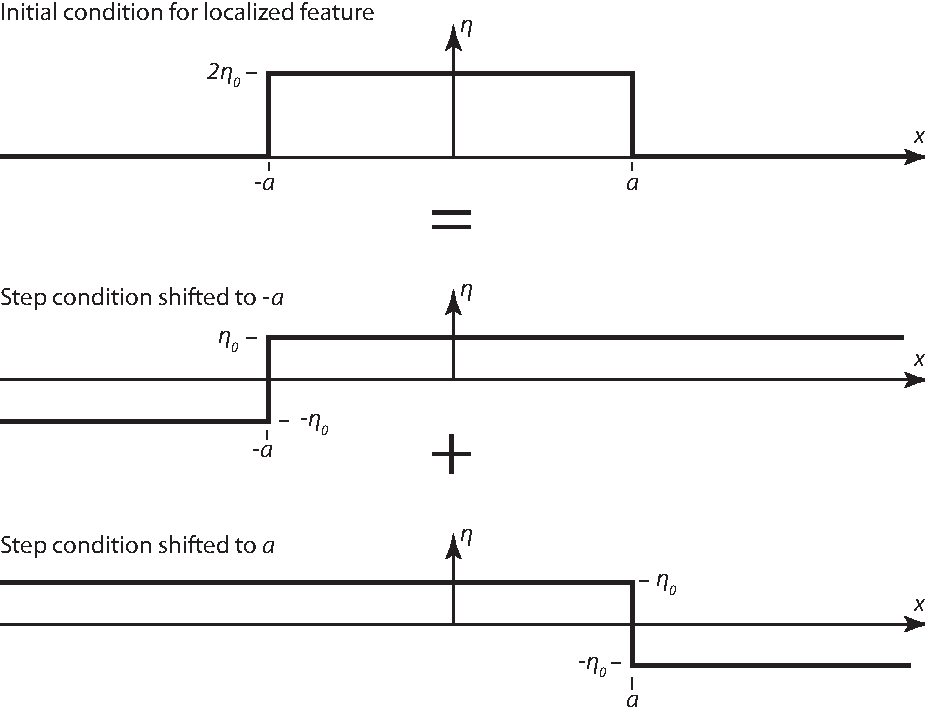
\includegraphics[width=5in]{tophat} 
    \caption{The initial condition for the localized feature adjustment problem, with the two step conditions that may be added to create the localized initial condition.  Summing the final condition for the two step conditions will then result in the final solution for the localized feature.}
    \label{fig:tophat}
\end{figure}

\subsubsection{Tophat adjustment}
\index{Adjustment problem:step}
The solution for an initial step for a non-rotating fluid will eventually produce a flat sea surface, \emph{i.e.}, all of the potential energy will be lost from the system.  A fundamental difference in the rotating system is that the potential energy is largely maintained within the system.  To explore this further, let us consider a slightly more complicated initial configuration, one in which a localized region with a width of $2a$ is raised $2\eta_0$ above an otherwise flat, quiescent sea.  A diagram of this configuration is shown in figure~\ref{fig:tophat}.  Note that the solution of this initial condition may be derived as the superposition of two laterally solutions to the initial step problem; this is also shown in figure~\ref{fig:tophat}.  The solution now has two initial step points, and thus three regions in which to calculate the solution.  The sea surface is given by
\begin{displaymath}
    \label{eq:tophat-solution}
    \eta =
    \begin{cases}
        \eta_0 \left( e^{(x+a)/Rd} - e^{(x-a)/Rd} \right)       & :  x < -a \\
        \eta_0 \left( 2 - e^{-(x+a)/Rd} - e^{(x-a)/Rd} \right)  & :  -a < x < a \\
        \eta_0 \left( -e^{-(x+a)/Rd} + e^{-(x-a)/Rd} \right)    & :  x > a .
    \end{cases}
\end{displaymath}
From this relationship, we can calculate the amount of potential energy retained in the system relative to the initial potential energy.  Here the potential energy at a point is defined as $PE = \rho_0\,g\,z$.  Integrating this vertically, from the sea floor to the sea surface gives
\begin{equation}
    \int_{-H}^{\eta} PE\,dz = \frac{1}{2}\rho_0\,g ( \eta^2 - H^2).
\end{equation}
However, we will only be concerned with the {\it available potential energy}.  There is a very large reservoir of potential energy, associated with the $H^2$ term, that is constant in time and is not available for conversion to kinetic energy.  We will define the potential energy of the ocean with $\eta=0$ as as our reference, the  and subtract it from our potential energy to get
\begin{equation}
    APE = \int_{-H}^{\eta} PE\,dz - \int_{-H}^{0} PE\,dz = \frac{1}{2}\rho_0\,g \eta^2.
\end{equation}
This expression can be integrated across the feature in the $x$-direction to an expression of the available potential energy per unit length of the feature (in the $y$-direction).  Initially, this is simply $\int_{-\infty}^{\infty} APE\,dx = 4 \rho_0\,g\,a\,\eta_0^2$.  The final $APE$ may also be calculated by integrating $\eta^2$ from equation~\ref{eq:tophat-solution}.  If this result is then normalized by the initial $APE$, the percentage of the potential energy retained follows the relation
\begin{equation}
    \frac{APE_{\mathrm{Final}}}{APE_{\mathrm{Initial}}} = 1 - \frac{3}{2a'} + \left( \frac{1}{2} + \frac{3}{2a'} \right) e^{-a'}
\end{equation}
where $a' = 2 a R_d^{-1}$, \emph{i.e.}, the total initial width of the feature normalized by the deformation radius\footnote{See the \emph{Mathematica} notebook {\tt tophat\_adjustment.nb} in the supplementary materials.}.  This solution is shown in figure~\ref{fig:APE_tophat}.  
% The limits of this equation are require L'Hospital's rule; note $(e^{-a'} - 1) a^{-1}|_{a'=0} = 1$.  
The percentage of the $APE$ retained when the feature width is much smaller than the deformation radius is zero.  This makes sense:  a glass of water poured into the ocean will not create a permanent feature.  On the other hand, essentially all of the $APE$ is retained when the feature is initially much larger than the deformation radius.  Thus, very large features are persistent in the ocean.  For a feature that is initially exactly the width of the deformation radius ($2 a = R_d$), the final state retains about~24\% of the initial $APE$.

\begin{figure}
    \centering
    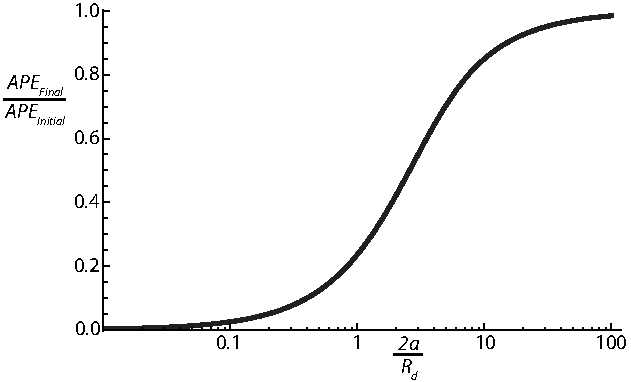
\includegraphics[width=4.0in]{APE_tophat}
    \label{fig:APE_tophat}
    \caption{The percentage of available potential energy retained in the final state, relative to the initial state as a function of the initial width of the feature for the tophat adjustment problem.}
\end{figure}

\subsubsection{Impulsive adjustment}
\index{Adjustment problem:impulse}
The final adjustment example shows how flow may be generated by forced lateral motion, similar to the way a conductor passing through a magnetic field generates current.  Consider a movable barrier oriented parallel to the $x$-axis in an ocean at rest.  As before, since there are no initial gradients or obstacles in the $x$-direction, we will assume that no gradients of any property develop in the $x$-direction.  The barrier acts as a piston, and pushes into the ocean a distance $\Delta y$.  To solve for the structure of the flow, we require a Lagrangian view of the fluid parcels touching the barrier, noting that the velocity of water at the wall is $v = D \Delta y /Dt$,
\begin{equation}
    \frac{Du}{Dt} - fv = \frac{D}{Dt}\left( u - f\,\Delta y \right) = 0 \; .
\end{equation}
Integrating in time from a state of rest gives 
\begin{equation}
    \label{eq:u_soln_impulse}
    u|_{y=\Delta y} = f\,\Delta y,
\end{equation}
thus a flow is generated along the edge of the barrier.  Since the potential vorticity of the fluid must be conserved, the solution of the flow seaward of the barrier is very similar to that already derived for the initial step.  Noting that far from the wall, the steady solution is $\eta|_{y\rightarrow\infty}=0$, the solution to equation~\ref{eq:linear-pv-conservation} is
\begin{equation}
    \eta = \eta_0 e^{-y/R_d} \; .
\end{equation}
with an associated velocity field
\begin{equation}
    u = \frac{g}{f}\eta_x = \eta_0 \sqrt{\frac{g}{H}} e^{-y/Rd}
\end{equation}
Now, we can determine the sea level at the coastal wall, $y = \Delta y$, using equation~\ref{eq:u_soln_impulse},
\begin{equation}
    \eta|_{y=\Delta y} = \frac{\Delta y\,H}{R_d}
\end{equation}
Note, that integrating the sea-level from the coastal wall outward, gives
\begin{equation}
    \int_{\Delta y}^{\infty} \eta\,dy = \Delta y\, H
\end{equation}
which is exactly the volume of water that was displaced by the motion of the wall.  The moving barrier pushes water into the coastal ocean, but this excess water is trapped near to the coast, with a trapping scale of the deformation radius.  Thus, both the amplitude of the sea level and the magnitude of the coastal jet are proportional to the magnitude of the barrier displacement.

\section{The Kelvin Wave}\index{Kelvin wave}

In this section, we will consider the most basic coastal wave.  The domain is a coastal region of constant depth, bounded on one side by a straight coastal wall oriented along the $x$-axis such that the offshore direction is in the positive $y$-direction.  We will use the linearized shallow water equations, but will retain time dependence.  The primary assumption is that the coastal constraint, no normal flow at the wall, or $v|_{y=0} = 0$, influences flow throughout the ocean, such that $v=0$ everywhere.  The governing equations under these simplifying assumptions are then
\begin{align}
    \frac{\partial u}{\partial t} &= -g\frac{\partial \eta}{\partial x} \label{eq:u-kelvin} \\
    f u &= -g\frac{\partial \eta}{\partial y}  \label{eq:v-kelvin} \\
    H\ \frac{\partial u}{\partial x} + \frac{\partial \eta}{\partial t} &= 0. \label{eq:cont-kelvin}
\end{align}
Equations~\ref{eq:u-kelvin} and~\ref{eq:cont-kelvin} may be combined, by eliminating $u$, to form the classic (non-rotating) shallow water wave equation, $\eta_{tt} = c^2 \eta_{xx}$.  Thus, very generally, we expect solutions to behave like shallow water gravity waves in the along-shore ($x$-) direction, with a phase speed of $c=\sqrt{g\,H}$.  The general form of the wave equation is
\begin{equation}
    \label{eq:wave-solution-kelvin}
    \eta = F_+(y) \phi_+(x - c t) + F_-(y) \phi_-(x + c t) = F_\pm(y) \phi_\pm(x \mp c t)
\end{equation}
The two {\it cross-shore structure functions}, $F_\pm(y)$, act as wave amplitudes for the two waves propagating in the $\pm x$-direction, and are still unknown.  The `plus' solutions represent waves propagating in the positive $x$-direction (later, we will call this direction {\it downcoast}), the `minus' solutions propagate in the negative $x$-direction ({\it upcoast}).  The waveforms follow {\it characteristics}, lines of constant phase, which are the arguments to the two wave solutions $\xi_\pm = x \mp c t$.

Now, combining the equations~\ref{eq:v-kelvin} and~\ref{eq:cont-kelvin}) by eliminating $u$ from both equations gives
\begin{equation}
    \label{eq:F-solution-kelvin}
    \frac{g H}{f} \eta_{x y} = \eta_t
\end{equation}
Plugging in our general solution form (equation~\ref{eq:wave-solution-kelvin})  into this differential equation gives for each wave propagation direction separately gives
\begin{align}
    \frac{g H}{f} \frac{\partial F_\pm}{\partial y} \phi_\pm' = \mp c \,F_\pm\,\phi_\pm'
\end{align}
Now, $\phi_\pm'$, the derivative with respect to the characteristic, $\xi=x \pm c t$ may be eliminated from both sides, to get a differential equation that defines the cross-shore structure function
\begin{equation}
    \label{eq:F-eqn-kelvin}
    \frac{\sqrt{gH}}{f} \frac{\partial F_\pm}{\partial y} = \mp F_\pm \; ,
\end{equation} 
with solutions
\begin{equation}
    F_\pm = N_0 e^{\mp y / Rd}.
\end{equation}
For solutions to remain finite as $x \rightarrow \infty$, only the decaying solution is valid.  

Although this is a very simple solution obtained under very restrictive assumptions, there are three aspects of this solution that are general to many other coastal wave problems.  First, this solution is associated with the positive characteristics, or the `plus' solution with waves traveling in the positive $x$-direction.  Waves traveling in the negative $x$-direction result in cross-shore structure functions that are unbounded, and are thus not permitted.  The cross-shore structure function thus constrains the waves to travel in only one direction.  This direction is the positive-$x$ direction in this example, but is generally a wave traveling with the coast to the right of the wave propagation direction in the northern hemisphere.  Coastal waves travel with the coast on their left in the southern hemisphere.  This direction is referred to as downcoast, the Kelvin wave propagation direction, or the shelf wave propagation direction.  Thus, information carried by large-scale waves about forcing conditions, a storm for example, travels downcoast with few exceptions.

Second, the waves are also bounded to the coast, or \emph{coastally trapped}, with maximum values of sea surface elevation at the coastal wall decaying offshore with characteristic scales of the deformation radius.  The flow is similarly bounded, such that the strongest currents are at the coast.  Note that equation~\ref{eq:v-kelvin} asserts that the along-shore flow, $u$, is geostrophic; the cross-shore flow was assumed to be zero.  The fact that these waves are trapped near the coast means that the Kelvin wave does not influence the circulation in the interior of the ocean, far ($y \gg R_d$) from the coastal wall.

Third, the general approach to the solution, assuming wave-like solutions in the along-shore direction, modulated by some cross-shore structure function that decays in the offshore direction is the typical approach for understanding periodic coastal flows.  With the inclusion of bathymetric variations, for example, there can be a series of cross-shore structure functions that solve the equation (cross-shore {\it modes} -- the Kelvin wave solution has only one mode).  In this case, the phase speed of each mode is related to the eigenvalue associated with that mode, such that different modes propagate at unique speeds.  However, the general form of the solution is identical:  a decaying function in the cross-shore direction modulating a wave-like solution in the along-shore direction.

An alternate derivation approach directly assumes a periodic solution with a specified wavenumber, $k$, in the along-shore direction; this often simplifies the derivation.  Let us assume a form of the solution
\begin{equation}
    \eta = F(y) e^{i(k x - \omega t)}
\end{equation}
We can plug this solution directly into equation\ref{eq:F-solution-kelvin}, and get
\begin{equation}
    \frac{g H}{f} k F_y = -\omega F
\end{equation}
Recall that $\pm \omega k^{-1} = \pm c = \pm \sqrt{g H}$ is the phase speed for shallow water gravity waves.  So, this equation reduces to
\begin{equation}
    \pm R_d F_y = - F
\end{equation}
which can be seen to be identical to equation~\ref{eq:F-eqn-kelvin}.  The only difference here is then that a particular wavenumber is chosen, so that the along-shore wave motions are sinusoidal, rather than a general waveform.  However, the waves are non-dispersive -- all wavenumbers travel at the same speed, $c=\sqrt{g H}$ -- an a general waveform may be constructed from a set of sinusoidal waveforms using Fourier decomposition.

\section{Divergence : Curl :: Waves : Vorticity}

We have seen in the two preceding examples, that we may find two classes of governing equations.  The general approach of eliminating the velocity variables to create a single equation in $\eta$ has two possible paths.  First, we can take an $x$-derivative of the $u$-momentum equation, a $y$-derivative of the $v$-momentum equation, and add these two equations.  This is similar to taking the {\it divergence} of the momentum equations.  There will be a flow divergence term resulting from the two acceleration terms that may exchanged using the continuity equation resulting in a $\eta_{tt}$ term.  The pressure terms here take a laplacian form.  Thus, taking the divergence of the momentum equations results in a wave-like equation, possibly with extra terms, depending on the assumptions made.

The other path is to take the {\it curl} of the momentum equations -- the $x$-derivative of the $v$-momentum equation minus the $y$-derivative of the $u$-momentum equation.  In this case, the pressure terms cancel because $\nabla \times \nabla \phi = 0$.  A divergence term is created from the two Coriolis terms, and this is exchanged using the continuity equation.  Taking the curl of the momentum equations results in a vorticity balance equation.

\section{A jet impinging on a coastal wall\\
\normalsize\citet{whitehead:85}}
\index{Jet!Impinging}

\begin{figure}[tb]
    \centering
    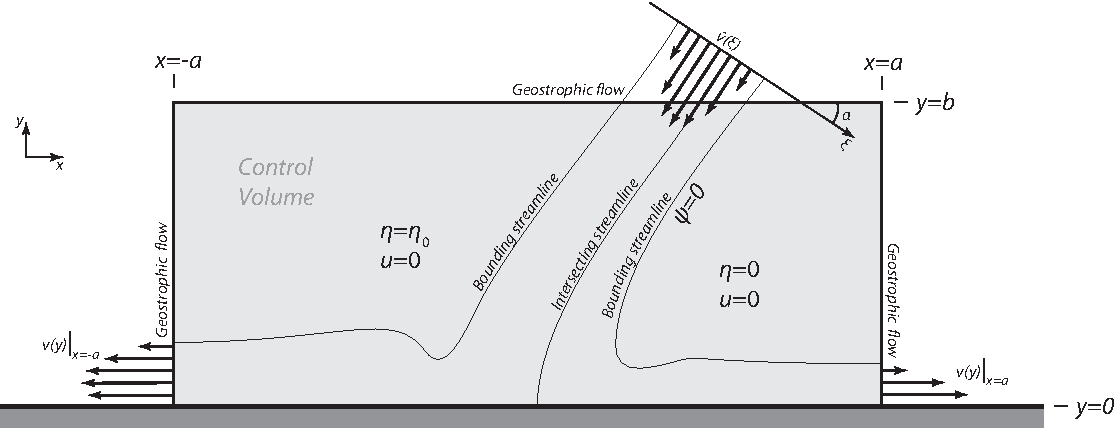
\includegraphics[width=6.5in]{impinging-jet} 
    \caption{The configuration of a jet impinging on a coastline, and the control volume used in the analysis of the resulting flow.  Note the angle, $\alpha$, shown in the figure is negative.}
    \label{fig:impinging-jet}
\end{figure}

Consider a geostrophic, barotropic jet, perhaps similar to the solution for the step adjustment problem, impinging on a coastal wall.  This example is based on a study by \citet{whitehead:85}, the primary difference being he examined a baroclinic jet, which is slightly more complicated.  We will examine the structure of the flow after the jet has come into contact with the wall by using a control volume approach.  A diagram of this configuration is shown in figure~\ref{fig:impinging-jet}.  We will assume the flow at the boundaries of the control volume is geostrophic, however, we allow for the possibility that the flow is non-linear within the control volume.  Also, as we will perform a momentum balance over this region, the advection of momentum in and out of the control volume will be critical in determining the evolution of the flow, thus, for this analysis the advective terms are retained.  For simplicity, however, we will only consider steady solutions.  Our governing equations are then
\begin{align}
    u u_x + v u_y - f v &= g \eta_x \label{eq:jet-u}\\
    u v_x + v v_y + f u &= g \eta_t \label{eq:jet-v}\\
    u_x + v_y &= 0. \label{eq:jet-continuity}
\end{align}
We will define a transport streamfunction, $\psi$, such that
\begin{equation}
    \psi_x = H v \quad ; \quad \psi_y = - H u.
\end{equation}
Note, that for geostrophic flow, but only for geostrophic flow, the streamfunction is proportional to the sea surface elevation, plus an integration constant, $\psi_0$
\begin{equation}
    \label{eq:eta_psi}
    \psi = \frac{g\,H}{f}\eta + \psi_0 \; .
\end{equation}
We are free to choose this integration constant, as the transport only depends on gradients of the streamfunction.  This integration constant is set to zero, $\psi_0 = 0$, so that $\eta=0$ regions are associated with $\psi=0$ regions.

The transport between two values of the stream function is constant, and depends only on the difference between the two streamfunction values, no matter how closely spaced or far apart these streamfunction contours are, since
\begin{equation}
    H \int_{\beta}^{\gamma} v\, dx = \psi\bigg|_{\gamma} - \psi\bigg|_{\beta}.
\end{equation}
A similar relation is also true for sea surface elevation, but only when the flow is geostrophic.

Using the continuity relation to rearrange the advective terms, and substituting streamfunction gradients for the velocity in the Coriolis terms, we get
\begin{align}
    (u^2)_x + (u v)_y - \frac{f}{H} \psi_x &= -g \eta_x \\
    (u v)_x + (v^2)_y - \frac{f}{H} \psi_y &= -g \eta_y.
\end{align}
Integrating the first equation, the $x$-momentum equation, over the control volume,
\begin{equation}
    \int_{-a}^a \int_0^b (u^2)_x + (u v)_y - f H^{-1} \psi_x + g \eta_x\;dx\,dy = 0.
\end{equation}
gives
\begin{equation}
    \int_0^b u^2 - f H^{-1} \psi + g \eta\;dy \bigg|_{x=-a}^a + \int_{-a}^{a} u v\;dx \bigg|_{x=0}^b = 0
\end{equation}
If we assume that, at $x=\pm a$ there is no flow normal to the coast, and that there are no along-shore gradients, the flow there must be geostrophic by equation~\ref{eq:eta_psi}, thus the $\eta$ and $\psi$ terms cancel.  Also, there is no flow normal to the wall at the coast, $v|_{y=0} = 0$, leaving,
\begin{equation}
    \int_0^b u^2 \;dy \bigg|_{x=a} 
        - \int_0^b u^2\;dy \bigg|_{x=-a}
        + \int_{-a}^{a} u v\;dx \bigg|_{y=b} = 0 \; .
\end{equation}
This statement requires that the integrated momentum flux through all of the open boundaries must balance.  The sign of each integral is set totally, for the first two terms, and in part, for the third term, by the direction of integration.  The conservation of along-shore momentum is more clearly stated if we set each integral such that the order of integration represents a positive momentum flux out of the control volume, \emph{i.e.}, integrating counter-clockwise around the control volume,
\begin{equation}
    \underbrace{\int_0^b u^2 \;dy \bigg|_{x=a}}_{\mathrm{Downcoast~outgoing}}
        + \underbrace{\int_b^0 u^2\;dy \bigg|_{x=-a}}_{\mathrm{Upcoast~outgoing}}
        = \underbrace{\int_{a}^{-a} u v\;dx \bigg|_{y=b}}_{\mathrm{Offshore~incoming}} \; .
\end{equation}
Notice that the advective terms are essential to this balance -- if the derivation is followed backwards, all three remaining terms in the final momentum balance can be seen to have originated in the advective terms.

Now, let us apply this balance to an arbitrary jet flowing in towards the coast, potentially at some angle, $\alpha$, skew to perpendicular.  Because the flow is geostrophic at the entry and exit points, the flow at a particular value of the streamfunction must have the same structure -- the same relative vorticity and sea surface elevation.  Thus, the presence of the coast splits the jet, but the branches of the jet eventually retain their original structure, with one branch exiting in the positive $x$-direction, and one branch exiting in the negative $x$-direction.  We can re-write the incoming flow in terms of a new coordinate, $\xi$, normal to the flow direction, defined as $\xi = x\,\mathrm{cos}(\alpha)$, where $\alpha$ is the angle between the two coordinates, $\xi$ and $x$.  This relation is a consequence of the fact that the span of the current in the $x$-direction is larger than it is in the $\xi$-direction for non-zero $\alpha$.  If we define the incoming flow, $\hat{v}$, is a function only of $\xi$, we can write the inflowing momentum as
\begin{equation}
    \int_{-a}^{a} u v\;dx = 
        \int_{-a}^{a} (\hat{v}\mathrm{sin}(\alpha))
                      (\hat{v}\mathrm{cos}(\alpha))\;\frac{d\xi}{\mathrm{cos}(\alpha)}
        = \mathrm{sin}(\alpha) \int_{-a}^{a} \hat{v}^2\;d\xi.    
\end{equation}
Next we need to determine the point in the incoming flow distribution that defines the point where the jet will split.  Because there is no flow normal to the coastline, the streamfunction along the coast is constant, since $\psi_x|_{y=0} = v|_{y=0} = 0$.  This coastal streamfunction is also the streamfunction that bisects the jet.  The reason that the streamfunction must be used to define this bifurcation point, instead of simply using $\eta$, is that the streamfunction may be guaranteed to be constant along the coastal wall, but $\eta$ is only constant if the flow is purely geostrophic. In other words, $\eta$ is not expected to be constant along the wall in the region where the jet hits the wall.  We may follow the coastal streamfunction value from the wall all the way up to the incoming geostrophic current, and as values of the streamfunction cannot cross for non-divergent flow this streamfunction separates the upcoast and downcoast flows.   Dividing the flow with respect to transport would not depend on the structure of the flow, a particular streamline divides the transport proportionally to the distance between the endmember streamfunctions that define the boundaries of the jet.  Here, we need to divide the flow with respect to momentum, \emph{i.e.}, $u^2$ instead of $u$, and this does depend on the details of the flow structure.  

Since the (single) incoming and two outgoing jets are geostrophic, we know that the streamfunction is directly proportional to the sea level elevation, $\eta$.  This means that the streamfunction and sea level elevation at the bifurcation point in the inflowing jet, and along the coast for the two outflowing jets are all identical, as $\psi$ is the same at all those locations.  In all cases the far-field conditions for both $\eta$ and $\psi$ are also shared between each side of the inflowing jet and the corresponding outflowing jet.  Because the flow is geostrophic, the relative vorticity may be written as $\zeta = g f^{-1} \nabla^2 \eta$.  Thus for each side of the inflowing jet, and each branch of the outflowing jets, we may write a boundary value problem in $\eta$, similar to equation~\ref{eq:step_adjustment_field}, based on the values either at the bifurcation point or along the coastal wall and the far field.  As the governing equations and boundary conditions are identical, it follows that the flow must have the same structure for each side of the incoming jet, and the corresponding outflow.

Because the structure of the flow is retained through the split -- at least in the outer regions where geostrophic flow may be assumed -- the axis perpendicular to the flow may be simply rotated to direct the incoming flow to be along-shore.  So, we can define the branch point with the equation using a single coordinate to define the the flow profiles,
\begin{equation}
    \int_{-a}^\Xi \hat{v}^2 \;d\xi - \int_\Xi^a \hat{v}^2\;d\xi = \mathrm{sin}(\alpha) \int_{-a}^{a} \hat{v}^2\;d\xi,
\end{equation}
and solve for $\Xi$, the point in the velocity profile where the flow will split.  This is straightforward to solve numerically for arbitrary flow profiles.  From this, the streamfunction and sea surface elevation structure of the two branches leaving the control volume may also be calculated.  Listing~\ref{lst:bifurcation}The following code calculates the bifurcation point.

\begin{lstlisting}[float=tp, 
                  caption={Numerical solution to find bifurcation point in a flow profile.  See {\tt split\_jet.py} for the full code.},
                  label=lst:bifurcation]
# An illustration of how to calculate the bifurcation point in a flow profile
# given the velocity, vhat, defined along the cross-flow coordinate, xi.
ip = np.trapz(vhat**2, xi)  # The total, integrated momentum

# Calculate the momentum at each point along the flow profile
ipi = np.empty_like(xi)
for n in range(1, len(xi)):
    ipi[n-1] = np.trapz(vhat[:n]**2, xi[:n])

ipi[n] = np.trapz(vhat**2, xi)

# Find the mid-point of the momentum profile, adjusted for the angle
# of the flow, alpha, such that the bifurcation point is defined by
# ipi=0
ipi -= 0.5 * (1 - np.sin(alpha)) * ip

# Find the lowest index with positive ipi
idx = np.argwhere(ipi >= 0)

# Now, find the bifurcation point, xo
if idx is None:
    xo = xi[-1]     # all transport goes right

i = idx.min()
if i == 0: 
    xo = xi[0]      # all transport goes left

# Linearly interpolat between the ipi points on either side of ipi=0
# to calcualte the exact position of the bifurcation, xo
yu = ipi[i]
yl = ipi[i-1]
xu = xi[i]
xl = xi[i-1]
xo = xl - (xu-xl)*yl/(yu-yl)
\end{lstlisting}





\subsection*{Further reading}

See problem~\ref{prob:step_wall_adjustment} for a comparison between non-linear solutions of a jet impinging on a wall, and combination of linear step adjustment and Kelvin wave solutions.\\

\noindent
Pichevin, T. and Nof, D. (1997). The momentum imbalance paradox. \emph{Tellus}, {\bf 49}A:298--319.\nocite{pichevin.nof:97}


\section{Frictional effects on vorticity}\index{Potential vorticity!Friction}

Normally, in fluid mechanics, boundary stresses are defined using the quadratic drag law, \emph{e.g.},  $\tau = c_D\,\rho\,u^2$.  The along-shore surface wind stress\footnote{{\it Kinematic stress} is used throughout for the surface wind stresses, $X$ and $Y$, with units of velocity squared, or m$^2$~s$^{-2}$.  Internal stresses, $\tau$, are defined as the {\it dynamic stresses}, with units of N~m$^{-2}$.  These quantities are related; the kinematic stress is simply the dynamic stress divided by the reference water density, $\rho_0$.}, for example, is defined as 
\begin{equation}
    X = \frac{\tau_{\mathrm{surface}}^{x}}{\rho_0} = c_D\, (\frac{\rho_{\mathrm{air}}} {\rho_0})\,|\mathbf{u}_{\mathrm{wind}}| u_{\mathrm{wind}} \; .
\end{equation}
Notice, for wind stress only only, the ratio of the air density, $\rho_{\mathrm{air}}$, to water density, $\rho_0$, since the \emph{dynamic} wind stress is determined by the density of air, $c_D\,\rho_{\mathrm{air}}|\mathbf{u}_{\mathrm{wind}}| u_{\mathrm{wind}}$.  For bottom stress,
\begin{equation}
    \frac{\tau_{\mathrm{bottom}}^{x}}{\rho_0} = c_D\, |\mathbf{u}_{\mathrm{near-bottom}}| u_{\mathrm{near-bottom}} \; .
\end{equation}
Technically, we should define the surface stress as the velocity differential between the air and water.  However, the wind stress is usually assumed to be specified by the wind speed alone --  an independent, specified forcing parameter -- since current speeds are typically so much smaller than wind speeds, so that the water may simply be considered to be stationary in the stress calculation.  The bottom stress, however, is proportional to the flow speed, which is part of the solution.  In order to ensure mathematically tractable problems, the bottom stress is often defined in simple analytical models as a linear stress, \emph{e.g.}, $\tau_{\mathrm{bottom}}^{x} \rho_0^{-1} = r\,u$, where $r$ is a linear friction coefficient.  The relationship between the linear and quadratic drag laws is then $r \simeq c_D u'$, where $u'$ represents high-frequency currents, unresolved by the model (\emph{e.g.}, tides), and is considered to be a specified parameter.  Typical values for $c_D$ are 1-3$\times$10$^{-3}$, and typical values for $r$ are 1-5$\times$10$^{-4}$~m~s$^{-1}$.  (Note, $c_D$ is non-dimensional, but $r$ is dimensional).  The vertically averaged stress terms in the momentum equations, $X h^{-1}$ and $r u h^{-1}$, arrises because the average vertical stress divergence, $(h \rho_0)^{-1} \int_{-h}^{\eta} (\tau_z)_z\,dz$ is a perfect integral, resulting in the difference between the surface and bottom stress terms divided by the total depth, $h+\eta \simeq h$.  Because of the small aspect ratio of the coastal ocean, we will ignore horizontal stresses for simplicity and only consider vertical stresses.

Let us revisit our derivation of the potential vorticity equation, done for the step adjustment problem, but this time, add bottom friction.  The governing equations are
\begin{align}
    \frac{\partial u}{\partial t} - f v
                &= -g\frac{\partial \eta}{\partial x} 
                    + \frac{X}{H} - \frac{r u}{H} \label{eq:u-shallow-linear-drag} \\
    \frac{\partial v}{\partial t} + f u
                &= -g\frac{\partial \eta}{\partial y} 
                    + \frac{Y}{H} - \frac{r v}{H} \label{eq:v-shallow-linear-drag} \\
    H\left(\frac{\partial u}{\partial x} + \frac{\partial v}{\partial y}\right)
        + \frac{\partial \eta}{\partial t} 
                &= 0. \label{eq:cont-shallow-linear-drag}
\end{align}
Following the same approach of taking the curl of the momentum equations, and substituting for the flow divergence using continuity, we arrive at
\begin{equation}
    \frac{\partial}{\partial t} \left( \frac{\zeta}{f} - \frac{\eta}{H} \right) = 
        \frac{1}{f H} \left( \nabla\times\mathbf{X} - r \zeta \right)
\end{equation}
where $\nabla\times\mathbf{X}$ is the curl of the wind stress.  Thus, potential vorticity is not conserved in the presence of friction.  A positive wind stress curl is associated with positive vorticity, and a depressed sea surface, this can be seen by imagining a divergent surface Ekman transport.  However, in coastal ocean dynamics, we typically ignore the wind stress curl.  Bottom friction reduces the magnitude of potential vorticity, and fills in or erodes local sea surface maxima.  This can be seen by considering the fact that bottom Ekman layer transport is toward the minimum for a local depression, and away from the maximum for a local high.  As the sea surface extremes are reduces, the associated geostrophic flow is also reduced, corresponding to a reduction in potential vorticity magnitude.

It is typically assumed that the effects of friction are limited to a thin surface and bottom boundary layer of thickness $\delta = \sqrt{\kappa\,f^{-1}}$.  In the interior of the water column, frictional effects are considered to be negligible; this is referred to as the {\it geostrophic interior}.  However, near the coast, as the bathymetry shoals, the surface and bottom boundary layers will eventually merge, and friction will become dominant throughout the water column.  This region is referred to as the {\it coastal boundary layer}.

\section{The Arrested Topographic Wave\\
\normalsize\citet{csanady:78}}
\index{Arrested topographic wave}

In this section, we will consider the steady state response of the ocean to a steady wind stress.  To ensure that currents do not accelerate without bound in response to the wind forcing, bottom friction must also then be included.  In practical terms, neither the forcing nor the response needs to be perfectly steady, but must have timescales much, much longer than the inertial period, $\partial/\partial t \sim \omega \ll f$.  In other words, approximately steady for timescales of a few days or longer.  

The steady shallow water equations, including both surface and bottom stresses are then
\begin{align}
    - f v &= -g\frac{\partial \eta}{\partial x} + \frac{X}{h} - \frac{r u}{h}   \label{eq:u-atwi} \\
     f u &= -g\frac{\partial \eta}{\partial y}  + \frac{Y}{h} - \frac{r v}{h}   \label{eq:v-atwi} \\
    \frac{\partial}{\partial x} (u h) + \frac{\partial}{\partial y} (v h) &= 0. \label{eq:cont-atwi}
\end{align}
We will assume that along-shore length scales are much longer than cross-shore length scales, $L_x \gg L_y$, typical for most continental shelves, and an assumption in all of the following examples.  This can also be written as $ k \sim \partial/\partial x \ll l \sim \partial / \partial y$, where $k$ and $l$ are the along- and cross-shore wavenumbers, respectively.  

The cross-shore momentum balance, equation~\ref{eq:v-atwi} is usually assumed to be in geostrophic balance, so that the two frictional terms are neglected in the cross-shore balance.  No such simplification is possible in the along-shore balance, equation~\ref{eq:u-atwi}.  This is because $u$ is assumed to be much larger than $v$, in particular,
\begin{equation}
    \frac{v}{u} \sim \frac{L_y}{L_x} \ll 1.
\end{equation}
If we assume that all of the terms in the along-shore equation are similar in magnitude, this implies that $f v h (r u)^{-1} \sim \mathcal{O}(1)$, which then requires $f u h (r v)^{-1} \sim L_x^2 L_y^{-2} \gg 1$.  Thus, we can neglect the bottom friction term in the cross-shore equation.  Assuming that the along-shore flow is in geostrophic balance with cross-shore sea surface gradients is very common in coastal dynamics problems; this assumption will be made in nearly all of the following examples as well.  That is, we will assume cross-shore wind stress is small compared to the two geostrophic terms, $Y h^{-1} \ll fu$.  Of course, since $Y$ is a specified forcing parameter, it cannot be {\it a priori} be eliminated through scaling.  However, the geostrophic terms, $fu$ and $\eta_x$, are both considered `large' terms in the scaling, and frictional terms are generally considered `small,' so there is some motivation for neglecting $Y$.  Ignoring cross-shore wind stress in the cross-shore momentum balance will be addressed in more detail in the next section on the wind-forced Kelvin wave by comparing along- and cross-shore forcing more explicitly to provide motivation for this assumption.  

We will assume that the atmospheric forcing is isotropic, that is the along- and cross-shore scales of the wind are similar, and both very large.  It will be this forcing scale that determines the shelf response to the wind, and will in part determine the along-shore scales of the flow.  So, while along-shore gradients in wind forcing may be important, we will neglect cross-shore gradients in wind forcing.  The shelf is assumed to be much narrower than the atmospheric forcing scales, and the along-shore wind may be considered to be uniform in the cross-shore direction.  In other words, we will neglect the wind stress curl.  While wind stress curl is an important aspect of wind forcing in the open ocean (\emph{e.g.}, Ekman pumping) wind stress curl is generally not considered important in coastal ocean dynamics. Rather the divergence of Ekman transport at the coast -- coastal upwelling and downwelling -- provides the principal forcing mechanism in wind-driven coastal circulation.

Another common assumption is that the bathymetry is uniform in the along-shore direction, and is a function of cross-shore distance alone, $h=h(y)$; we will also make this assumption in all of the following examples.  This assumption is almost essential for mathematically tractable problems.  If along-shore variations in bathymetry are determined to be important, however, the simplest way to include such variations is to assume that the bathymetry is self-similar, and is a function of percent distance across the shelf.  Mathematically, this is done with a transformation of variables, $h=h{y^*}$, where $y^*=y/b(x)$ is the cross-shelf coordinate normalized by the variable shelf width.  All of the variables must be transformed in this way.  This complicates the equations, but it may still be possible to find analytic solutions.

Thus, with the above simplifications applied, the governing equations become
\begin{align}
    - f v &= -g\frac{\partial \eta}{\partial x} + \frac{X}{h} - \frac{r u}{h}   \label{eq:u-atw} \\
     f u &= -g\frac{\partial \eta}{\partial y} \label{eq:v-atw} \\
    h \frac{\partial u}{\partial x} + \frac{\partial}{\partial y} (v h) &= 0. \label{eq:cont-atw}
\end{align}
The simplest approach is to multiply the two momentum equations by $h$ to create transport equations, and then take the curl of these equations.  Use geostrophy to write $r u h^{-1}$ in terms of $\eta$ and substitute into the continuity equation, to get
\begin{equation}
    \label{eq:atw}
    \eta_x - \frac{r}{f h_y} \eta_{yy} = 0.
\end{equation}
This vorticity equation has the form of a heat equation $\phi_t - \kappa \phi_{xx} = 0$.  Thus, there is a direct analogy between sea level elevation and heat conduction in a rod.  The cross-shore direction is analogous to the coordinate along the length of the rod, time is analogous to the positive $x$-direction (\emph{i.e.}, the downcoast direction, in the direction of Kelvin wave propagation), and $f h_y r^{-1}$ is related to the heat conduction coefficient, $\kappa$.  

The analogy with time indicates that the direction of influence in the arrested topographic wave model is downcoast, just as in the Kelvin wave model.  Just as it is impossible for later events to influence prior solutions in the heat conduction equation -- the heat conduction equation is not well posed for integrating backwards in time -- localized forcing in the arrested topographic wave model may only influence circulation in the downcoast direction.  Upcoast regions are unaffected by forcing that occurs downcoast.  As we have seen before, this is a consequence of ignoring the advective terms.

If we somehow force a strong, narrow current along the coast with strong cross-shore gradients in $\eta$, we expect this current to diffuse or broaden in the downcoast direction.  The rate of this diffusion will be inversely proportional to gradients in potential vorticity, $f h_y h^{-1}$; stronger potential vorticity gradients tend to preserve the vorticity inherent in the current.  The rate of diffusion will be proportional to $r h^{-1}$, the inverse timescale of bottom drag on the flow, which tends to smear out and destroy vorticity.  Strong rotation and steep bathymetric gradients impede flow from crossing isobaths; recall for inviscid geostrophic flow, currents are required to follow the isobaths exactly.  Bottom friction, proportional to $r$, breaks this constraint by modifying the local potential vorticity and allowing the flow to cross isobaths.

Notice that the wind forcing does not appear in equation~\ref{eq:atw}.  This is because the curl of the wind stress is assumed to be small; the wind forcing enters the problem at the coastal boundary.  At the coastal wall, there can be no flow normal to the coast, $v=0$.  Also, we will assume that the bathemetry shoals near the coast, such that $h|_{y\rightarrow 0^+} \rightarrow 0$.  As the bathemetry gets shallower, the two friction terms get proportionally larger.  Eventually, they become the two dominant terms, and must balance, $X = ru$, or
\begin{equation}
    \frac{\partial \eta}{\partial y} = -\frac{X}{r g} .
\end{equation}
Note, while the along-shore balance is entirely frictional, the cross-shore balance is still geostrophic.  It often occurs in coastal oceanography that the along- and cross-shore balances have fundamentally different characters.

TODO:
\begin{itemize}
    \item Two examples from numerical solution
    \item Scaling arguments
\end{itemize}


\begin{lstlisting}[float=tp,
                   caption={Arrested topographic wave numerical solution kernel.  See {\tt atw.py} for the full code.},
                   label=lst:atw]
fac1 = (dx / dy**2) * (r / (f * h_y[1:-1]))
fac2 = dy / (r * g)
for n in range(1,Nx):
    # The interior solution governed by heat equation
    eta[1:-1, n] = eta[1:-1, n-1] +  fac1 * np.diff(eta[:,n-1], n=2)
    # The coastal boundary condition
    eta[0, n] = eta[1, n] + fac2 * X[n]
    # The offshore-boundary condition
    eta[-1, n] = eta[-2, n]
\end{lstlisting}


\section{Wind-forced Kelvin wave}
\index{Kelvin wave!wind forced}

Here, consider a homogeneous coastal ocean of constant depth, $h=H$,  with a coastal wall -- the same domain as in the Kelvin wave solution.  We will consider a time-dependent solution, but will ignore bottom friction.  We will assume flow frequencies much longer than an inertial period, $ \omega \ll f$, and that the along-shore scales are much larger than cross-shore scales, $L_x \gg L_y$.  With these assumptions it is clear to see that
\begin{equation}
    \frac{ \frac{\partial v}{\partial t} }{ f u } \sim \frac{ \omega L_y}{ f L_x } \ll 1,
\end{equation}
so that the cross-shore acceleration term, $v_t$, may be ignored.  Thus, the cross-shore balance is again geostrophic at least for the commonly considered case of purely along-shore winds.  To make the analysis simpler, let us also assume that the wind stress is spatially uniform, although possibly varying in time.  This assumption is equivalent to assuming that the horizontal spatial scales of the wind are much larger than the spatial scales of flow in the coastal ocean.  For many coastal regions, for example the south and east U.S., and northern European coastal regions, this is a good assumption.  However, there are many counter examples; coastal mountain ranges may cause winds with very small scales: the marine boundary layer along the U.S. west coast, \emph{bora} winds in the adriatic, and the Papagayo jet in Central America.

Since there are no along-shore gradients in the initial condition or in the forcing, and since the coastal wall is oriented perfectly along-shore, we may assume that no along-shore gradients develop in any property, $\partial / \partial x = 0$.  The governing equations are then,
\begin{align}
\frac{\partial u}{\partial t} - fv &=  \frac{X}{H} \label{eq:u-forced-kelvin} \\
    f u &= -g\frac{\partial \eta}{\partial y} + \frac{Y}{H} \label{eq:v-forced-kelvin} \\
    H\ \frac{\partial v}{\partial y} + \frac{\partial \eta}{\partial t} &= 0. \label{eq:cont-forced-kelvin}    
\end{align}
For the moment, we will allow for wind stress in either the along- or cross-shore direction, but will treat these two cases separately.  

First consider the along-shore wind stress case.  At the coast, $v=0$, so the $x$-momentum equation becomes $u_t = X H^{-1}$.  Thus, the along-shore flow at the coast proportional to the time integral wind stress; the along-shore flow is balanced by a cross-shore pressure gradient since the cross-shore balance is geostrophic.  There are two important consequences of this balance.  First, under steady wind forcing, the along-shore current undergoes constant acceleration, and increases linearly in time.  Thus, the response of the flow to wind forcing is proportional not only to the magnitude of the wind stress, but also the duration.  Second, since the current depends on the time history of the wind stress, the wind stress at any given time does not determine the flow.  In particular, given a wind event of finite duration, the along-shore flow continues even after the wind ceases.  This is because the along-shore flow is generated by the wind, but is balanced by the cross-shore pressure gradient, and so does not require continued wind forcing to be maintained; when the wind ceases, the geostrophic flow persists.

Next, consider the cross-shore wind stress case.  The steady solution (ignoring transients) is simply Ekman transport in the along-shore direction, $u = (f H)^{-1} Y$.  No sea-level gradients are required, as the flow is in direct balance with the wind stress.  If the Ekman transport near the coast is suppressed  by bottom friction, a sea-level gradient counter to the wind stress may form, but this is also steady and in direct balance with the wind stress.  Thus, cross-shore wind stress generates a current proportional to the instantaneous wind stress that vanishes when the wind ceases.

Given along- and cross-shore wind stresses of similar magnitude, the ratio of the along-shore current generated by the cross-shore, $u_Y$, wind to the along-shore current generated by the along-shore wind, $u_X$ will be
\begin{equation}
    \frac{u_Y}{u_X} \sim \frac{\omega}{f} \ll 1.
\end{equation}
For this reason, the cross-shore wind forcing is ignored in many models of coastal ocean circulation, and in the following discussion, we will focus on along-shore wind forcing only.

Create a vorticity equation by taking the curl of the equations, to get
\begin{equation}
    \eta_t + \frac{gH}{f^2} \eta_{yyt} = 0.
\end{equation}
Notice, that again the wind forcing does not come into the vorticity equation, but rather through a boundary condition.  Integrate this equation in time to get a differential equation, with the familiar, exponentially-decaying cross-shore structure function as the solution.  Ignoring the cross-shore wind provides the coastal boundary condition at $y=0$,
\begin{equation}
    \frac{\partial \eta}{\partial y} = - \frac{f}{g H} \int_0^t X\,dt'.
\end{equation}
The far-field limit, $y\rightarrow \infty$, is naturally $\eta \rightarrow 0$.  Given that we know the structure of sea level elevation in the cross-shore direction, $\eta = \eta_0 e^{-y/R_d}$, we may solve for $\eta_0$, the coastal sea level
\begin{equation}
    \eta_0 = \frac{1}{\sqrt{g H}} \int_0^t X\,dt'.
\end{equation}

The build-up of water at the coast is exactly equal to the Ekman transport coming in from the far field.  Very far from the coast, $y R_d^{-1} \gg 1$, the sea level is flat, so by the cross-shore geostrophic balance, $u=0$.  The along-shore balance is then just the Ekman transport toward the coast, $u H = X f^{-1}$, per unit width of the coastline.  The change in the excess volume associated with sea level changes near the coast, $\Delta V$, again per unit width of the coastline, is
\begin{equation}
    \frac{\partial \Delta V}{\partial t} = 
    \frac{\partial}{\partial t} \int_0^\infty \eta_0 e^{-y / R_d}\,dy =
        \frac{\partial}{\partial t} (\eta_0\,R_d) = 
        \frac{\partial}{\partial t} \frac{Rd}{\sqrt{g H}}\int_0^t X\,dt' = \frac{X}{f} 
\end{equation}
Thus, the change in volume near the coast is exactly equal to the incoming, far-field Ekman transport.

The next stage in complexity is to allow along-shore gradients in the along-shore wind.  However, this problem is left as an exercise, and we will pursue the more general problem that also includes cross-shore variations in bathymetry in the next section.  

\section{Continental Shelf Waves\\
\normalsize{\citet{gill.schumann:74}}}
\index{Continental shelf waves}

We will use a similar set of assumptions for continental shelf waves as for the wind-forced Kelvin wave problem.  We will still consider long time scales, $\omega \ll f$, assume along-shore scales are much larger than cross-shore scales, $L_x \gg L_y$, and ignore cross-shore wind stress.  We will continue to ignore bottom friction, although our experience with the arrested topographic wave model suggests this assumption may be poor.  However, we will relax two assumptions, and allow for along-shore variations in the flow, and allow for cross-shore bathymetric variations.  

\begin{align}
    \frac{\partial u}{\partial t} - fv &=  - g \frac{\partial \eta}{\partial x} + \frac{X}{h} \label{eq:u-csw} \\
        f u &= -g\frac{\partial \eta}{\partial y} \label{eq:v-csw} \\
        \frac{\partial}{\partial x}(u h) + \frac{\partial}{\partial y}(v h) + \frac{\partial \eta}{\partial t} &= 0. \label{eq:cont-csw}    
\end{align}
We can take the curl of the momentum equations, after multiplying by $h$, and use the continuity relation to get
\begin{equation}
     \underbrace{ \frac{\eta_t}{f} }_{\omega f^{-1}}
        - \underbrace{ \left( \frac{g h}{f^3} \eta_{yt} \right)_y }_{ \omega f^{-1} \; R_d^2 L_y^{-2} }
        + \underbrace{ \frac{gh_y}{f}\eta_x }_{R_d^2 L_x^{-1} L_y^{-1}} = 0
\end{equation}
where the scales of each term are indicated below each term in the equation.

A key parameter will be the cross-shelf scales in relation to the deformation radius, $L_y R_d^{-1}$.  Given a scale depths between $H=10$ and 100~m, and given a typical mid-latitude Coriolis parameter of $f=10^{-4}$~s$^{-1}$, the deformation radius ranges from 100 to 300~km.  This is also the typical shelf width of many wider continental shelves.  Given our experience with the Kelvin wave, we expect the response of the shelf to wind forcing to be trapped near the coast, so it is often assumed that the dynamical, cross-shelf scales of continental shelf waves are smaller than the deformation radius.  Since the sea surface is only flexible or pliable at scales of the deformation radius, or larger, this means that the sea surface in the continental shelf wave solution will be relatively stiff.  Thus, the first term in the vorticity equation, stemming to the $\eta_t$ term in the continuity equation, above may be ignored.  In other words, the stiffness of the sea surface requires that the flow is essentially non-divergent.

The final term in the vorticity equation may also be small.  While the cross-shore scale, $L_y$, is determined by a combination of the shelf geometry and the system dynamics -- by the solution of the cross-shore structure function -- the along-shore scale, $L_x$, is determined by the along-shore scales of the forcing.  However, assuming that along-shore gradients are important, and that the two remaining terms in the vorticity equation are of similar magnitude, we see that $\omega f^{-1} L_x \sim L_y$, so that even in this case, along-shore scales are much longer than cross-shore scales.  We will assume that this scale represents the smallest along-shore forcing scales, and as such, we will not further restrict the problem by neglecting this term.

The assumption that the flow is nearly non-divergent may be used to recast the above equation in terms of the transport streamfunction,
\begin{align}
        \psi_x &= v h \\
        \psi_y &= -u h
\end{align}
(The streamfunction is not defined for divergent flows.)  Casting the vorticity equation in terms of the transport streamfunction has one large advantage over the equation in $\eta$ -- the boundary conditions are much simpler.  For $\eta$, while the offshore boundary condition is quite simple ($\eta|_{y\rightarrow\infty} \rightarrow 0$), the coastal boundary condition is complex,
\begin{equation}
    g \eta_x - \frac{g}{f}\eta_{y t} = \frac{X}{h} \quad \mathrm{at} \quad y=0.
\end{equation}
The potentially small term, the first of the two $\eta$ terms may be not be neglected if we assume that along-shore gradients in the vorticity equation are retained.  Thus, there is no straigtforward simplification to be made.  However, the boundary conditions on the transport streamfunction equation are quite simple, no cross-shore flow at the coast
\begin{equation}
    \psi_x\bigg|_{y=0} = 0,
\end{equation}
and no along-shore flow very far from the coast
\begin{equation}
    \psi_y\bigg|_{y\rightarrow\infty} = 0.
\end{equation}
Again, there is an arbitrary constant in the definition of the transport streamfunction that we are free to choose.  We will select $\psi=0$ along the coastal wall to define this constant, and use this relation as an even simpler coastal boundary condition.  

The transport streamfunction vorticity equation is derived by eliminating $\eta$ from the two momentum equations, substitute the velocities for gradients in $\psi$, and use the assumption that the transport must be non-divergent to get
\begin{equation}
    \label{eq:psi-csw}
    \left( \frac{\psi_y}{h} \right)_{y t} - \frac{f h_y}{h^2}\psi_x = \frac{h_y}{h^2}X
\end{equation}
Note, that the wind appears here as a non-homogeneous forcing term in the $\psi$ vorticity equation, whereas it was not present in the $\eta$ vorticity equation.  In the $\eta$ vorticity equation, forcing enters through the coastal boundary condition.  In the $\psi$ vorticity equation, the coastal boundary condition, $\psi=0$, is the same regardless of the forcing because of the coastal constraint.  However, far from the coast, the geostrophic portion of the flow vanishes, but there is still Ekman transport due to the wind stress, so that $\nabla\eta = 0$ there, but $\nabla\psi \ne 0$.  Thus the $\eta$ and $\psi$ vorticity equations pin down the solution at different points, $\eta=0$ far from the coast with the maximum variability at the coast, whereas $\psi=0$ at the coast with the maximum variability far from the coast.

We will solve the homogeneous ($X=0$) transport streamfunction vorticity equation~(\ref{eq:psi-csw}) first by separation of variables.  Let $\psi(x, y, t) = \phi(x, t) F(y)$.  Plugging this definition into equation~\ref{eq:psi-csw}, and placing $\psi$ and $F$ on opposite sides of the equation, gives
\begin{equation}
    \frac{\phi_t}{\phi_x} =  \frac{\frac{f h_y}{h^2} F }{\left( \frac{F_y}{h}  \right)_y} = -c
\end{equation}
The constant, $c$, has a negative sign because it will be demonstrated below that, written so, $c$ must be positive.  Because the first relation only depends on $\phi$, and the second only on $F$, each must be constant.  The first relation is then
\begin{equation}
    \phi_t + c\phi_x = 0
\end{equation}
which is the transport equation showing uniform propagation of a feature upcoast with a phase speed $c$.  The along-shore part of the solution is then
\begin{equation}
    \phi(x, t) = \Phi(x - ct)
\end{equation}
a feature with an initial distribution $\Phi(x)$, propagating in the Kelvin wave direction without dispersion.  Thus, $c$ may be interpreted as a phase speed.

The next relation
\begin{equation}
    \label{eq:F-csw}
      - \left( \frac{F_y}{h}  \right)_y   = c^{-1} \frac{f h_y}{h^2} F
\end{equation}
is a Strum-Liouville eigenvalue problem, where in standard notation, $\lambda = c^{-1}$, $p(x)=h^{-1}$, $q(x)=0$, and $w(x)=f h_y h^{-2}$.  The properties of this class of equation are well known.  There will be an infinite number of solutions, $F_i$, called {\it eigenfunctions} or {\it modes}, each corresponding to a particular {\it eigenvalue}, $c^{-1}_i$.  Thus, each mode has a distinct phase speed, $c_i$.  The eigenvalues are all positive definite, and  increase monotonically for increasing mode.  The eigenfunction associated with each increasing value of the eigenvalue has successively more zero crossings.  Thus, the lowest mode has a structure such that the currents are all directed one way over the whole shelf.  Higher modes have current reversals in the offshore direction, more for increasing mode number.  As the eigenvalues, $c^{-1}_i$, increase for increasing mode, we see that higher modes correspond to lower phase speeds; the lowest modes propagate the fastest.  Perhaps the most powerful feature of the solution, however, is that all of the modes are orthogonal, so that any function may be decomposed into a unique series of eigenfunctions, like a Fourier decomposition, but with a different set of basis functions.

This equation may be solved numerically, or analytically for certain simple choices of bathymetry.  Here, let us present solutions for two simple choices of bathymetry to demonstrate some of the solution characteristics.  The first is an exponentially increasing shelf depth
\begin{equation}
    h = H e^{2 \gamma y}
\end{equation}
where $L$ and $H$ are numbers that characterize the shape of the shelf.  The general solution to equation~\ref{eq:F-csw} is
\begin{equation}
    \label{eq:F-sol-csw}
    F_i = A_i e^{\gamma y} \mathrm{sin}(\beta_i y)
\end{equation}
where we have used the coastal boundary condition $F=0$ to eliminate the cosine solution.  The boundary condition at the shelf edge $F_y = 0$ at $y=L$ can be used to solve for $\beta_i$
\begin{equation}
    \gamma \mathrm{sin}(\beta_i L) + \beta_i \mathrm{cos}(\beta_i L) = 0
\end{equation}
Plugging equation~\ref{eq:F-sol-csw} into equation~\ref{eq:F-csw}, the resulting equation evaluated at the coast, $y=0$, relates $\beta_i$ and $c_i$
\begin{equation}
    c_i = \frac{2 \gamma f}{\beta_i^2 + \gamma^2}.
\end{equation}

The other class of bathymetry is a linear depth profile
\begin{equation}
    h = \alpha y
\end{equation}
which has solutions that include second-order Bessel function of the first kind
\begin{equation}
    F_i = A_i \frac{y}{R_{di}} J_2 \left( \sqrt{\frac{y}{R_{di}}} \right)
\end{equation}
where 
\begin{equation}
    R_{di} = \frac{c_i}{f}
\end{equation}
The solutions of
\begin{equation}
    J_2 \left( \sqrt{\frac{L}{R_{di}}} \right) + \frac{L}{4 R_{di}}\left[ J_1\left( \sqrt{\frac{L}{R_{di}}} \right) - J_3\left( \sqrt{\frac{L}{R_{di}}} \right) \right] = 0
\end{equation}
determine $R_{di}$, which can be used to determine $c_i$.  Of course, this sort of ridiculous expression is best solved numerically.  Note a curious aspect of this solution is that it does not depend on the bathymetric gradient, $\alpha$ -- it only matters that the slope is constant, it does not matter what the value of that slope is.

So, let us proceed as if we have already somehow calculated the eigenvalues, the values of $c_i$. The final part of the problem is to determine the amplitude of each mode, making use of the fact that all of the eigenfunctions are orthogonal.  The first step is to determine an integral that defines this orthogonality.  Multiply equation~\ref{eq:F-csw} for a specific mode, $F_i$, by a potentially different mode $F_j$, and {\it vise verse}.  Subtract these two equations to get
\begin{equation}
     F_i\left( \frac{F_{jy}}{h}  \right)_y + c_i^{-1} \frac{f h_y}{h^2} F_i F_j
   - F_j\left( \frac{F_{iy}}{h}  \right)_y - c_j^{-1} \frac{f h_y}{h^2} F_j F_i = 0
\end{equation}
Now, integrate this equation in y over the entire shelf from $y=[0, L]$.  Integration by parts and application of the boundary conditions causes the two terms with $y$-gradients to vanish, leaving the relation
\begin{equation}
    \left( c_i^{-1} - c_j^{-1} \right) \int_0^L \frac{h_y}{h^2} F_i F_j \, dy = 0.
\end{equation}
Either $c_i^{-1} - c_j^{-1} = 0$, indicating that the two modes are actually the same, or the integral vanishes, meaning that the two modes are orthogonal.  These eigenfunctions must be normalized, defining the value of the integral when it is not zero.  We will do so using the relation
\begin{equation}
    \int_0^L \frac{h_y}{h^2} F_i F_j \,dy = \delta_{ij}
\end{equation}
where $\delta_{ij}$ is the Kroneker delta function: $\delta_{ii} = 1$, $\delta_{ij}=0$ when $i \ne j$.  If we now define the (weighted) integral of a single eigenfunction to be
\begin{equation}
    \label{eq:csw-mode-norm-amp}
    b_i = \int_0^L \frac{h_y}{h^2} F_i\,dy
\end{equation}
then the useful orthogonality relation
\begin{equation}
    \label{eq:csw-flatforce}
    \sum_{i=0}^\infty b_i F_i = 1
\end{equation}
can be demonstrated by multiplying both sides by $h_y h^{-2} F_j$ and integrating.

The governing equation including wind forcing is then, after using the separated variables
\begin{equation}
   \sum_{i=0}^\infty \left[ \phi_t \left( \frac{F_{iy}}{h} \right)_{y} - \frac{f h_y}{h^2} \phi_x F_i \right]= \frac{h_y}{h^2} X
\end{equation}
First use equation~\ref{eq:F-csw} to write the first term in the sum without gradients in $F$, and including the phase speed, $c$.  Then, multiply the whole equation by $F_j$, integrate from $y=[0, L]$, (recall that we have assumed that $X$ does not depend on $y$), and apply the orthogonality relations derived above to get
\begin{equation}
    c_i^{-1} \phi_t + \phi_x = -b_i \frac{X}{f}
\end{equation}
Solutions are then found by integrating the forcing, $X f^{-1}$, along a constant characteristic
\begin{equation}
    s = t - \frac{x}{c_i} = \mathrm{const.}
\end{equation}
While such a solution is conceptually straightforward, it can be mathematically cumbersome, so we will abandon our analytical derivations here, and proceed with a discussion of the solution.

The wind forcing is assumed constant across the shelf, so that equation~\ref{eq:csw-flatforce} is applicable.  The decomposition of the wind forcing by equation~\ref{eq:csw-mode-norm-amp} shows how each mode is excited by the wind stress.  As the wind is constant across the shelf, this is a function only of the wind stress amplitude.  Each mode, however, travels at a different speed, $c_i$.  When the wind forcing is integrated along a characteristic, the history of wind forcing is different for each characteristic because each travels along a different path separated by differing speeds.  



\section{Hydraulic control}
\index{Hydraulic control}
\index{Flow!Supercritical, subcritical}

The final section in this chapter is a departure from rotating flows.  Here, we will examine hydraulic control at a constriction in a channel.  Although barotropic hydraulic control rarely happens in the ocean, it is a important and relevant because it provides intuition for more complicated hydraulic flows, and it is directly applicable to hydraulically controlled baroclinic flows with a single active layer.

Assume a non-rotating channel with possible variations in bathymetry, $m$, and width, $b$; we will treat variations in bathymetry and width separately.  Here, to keep in line with the notation used in hydraulic control problems, we will reserve $h$ for the fluid thickness.  Assume that there are no cross-channel variations in flow or in they bathymetry, so that all variables are only a function of the along-channel coordinate, $x$.  Let the fluid be uniform density, and assume that the flow is steady.  We will examine steady flow resulting from an initial dam break, so that the flows may potentially be quite strong, and so the advective term will be retained.  Also, changes in sea surface elevation may be similar in magnitude to bathymetric changes, so the continuity equation will conserve the total volume flux, $Q=u h b$, where $h=\eta-m$ is the thickness of the fluid layer.  The governing equations are then an along-channel momentum equation and continuity
\begin{align}
    u \frac{\partial u}{\partial x} &= -g \frac{\partial \eta}{\partial x} \\
    \frac{\partial}{\partial x}(u h b) &= 0
\end{align}

\begin{figure}[tb]
    \centering
    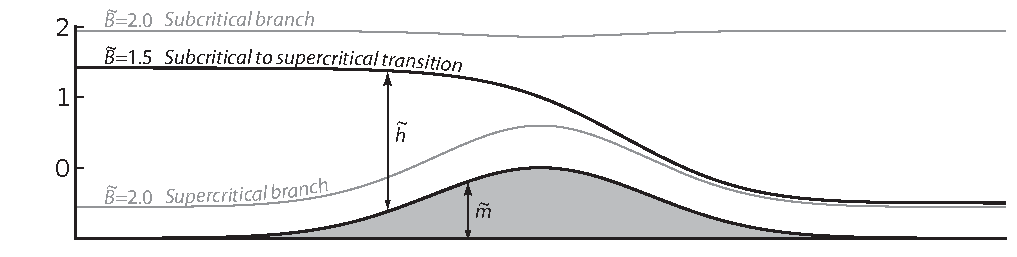
\includegraphics[width=6in]{hydraulic} 
    \caption{Two classes of solutions are shown.  The asymetrical case of subcritical to supercritical flow is shown by the thicker line, and is associated with $B=3/2$.  Two solutions for $B=2$ are shown in thin grey lines.  One is for the supercritical branch, one for the subcritical branch.  Note that the maximum value of $m$ is zero, $m$ is negative elsewhere.  See text for details.}
    \label{fig:hydraulic}
\end{figure}

Let us consider variations in bathymetry first, so that $b_x = 0$, and the continuity equation becomes $(u\,h)_x = 0$.  The first step will be to separate (known) changes in the bathymetry from (unknown) changes in the fluid thickness, $h$, in the momentum equation
\begin{equation}
    \label{eq:bump-u}
    u \frac{\partial u}{\partial x} + g \frac{\partial h}{\partial x} = - g \frac{\partial m}{\partial x}
\end{equation}
Now, eliminate $u$ using the continuity equation to get
\begin{equation}
    h_x (Fr^2 - 1) = m_x 
\end{equation}
where
\begin{equation}
Fr^2 = \frac{u^2}{g h}.
\end{equation}
At the peak of the obstacle, at $m_x = 0$, either $h_x = 0$ or $Fr^2 = 1$.  Assume there is a bump separating a full reservoir from an empty reservoir.  In this case the flow must be asymmetric, so that $h_x \ne 0$, and $Fr^2 = 1$ at the peak.

Now, integrate the momentum equation~\ref{eq:bump-u} in $x$, after substituting $u u_x = \frac{1}{2}(u^2)_x$, to get
\begin{equation}
    \frac{u^2}{2} + g h + g m = B
\end{equation}
where the integration constant, $B$, is known as the \emph{Bernoulli} constant, since this equation is a form of Bernoulli's equation.  Now, define the mass transport as $Q=u\,h\,b$, and rearrange to get
\begin{equation}
    \label{eq:bernoulli-dim}
    \frac{Q^2}{2 b^2 h^2} + g h = B - g m.
\end{equation}
Far from the bump, on the full side of the reservoir, let us assume that $u=0$, $h=H$, and $m=0$, so that $B = g H$.  Thus, $B$ is the total \emph{Bernoulli head}, and $B-gm$ is the \emph{available} Bernoulli head, defining the potential energy of the quiescent water in the far field above the height of the obstacle, $m$.  Note, when $B - gm \le 0$, the flow is completely blocked by the obstacle.

In order to investigate equation, it is necessary to non-dimensionalize the variables.  Otherwise, we would be required to choose arbitrary dimensional parameters in order to plot the equation.  Let $h=D\tilde{h}$ and $m=D\tilde{m}$, so that
\begin{equation}
    \frac{Q^2}{2 g b^2 D^3}\frac{1}{\tilde{h}^2} + \tilde{h} = \frac{B}{g D} - \tilde{m}.
\end{equation}
Thus, if we now let $D = Q^{2/3} b^{-2/3} g^{-1/3}$, and $\tilde{B} = B (g D)^{-1}$, we have
\begin{equation}
    \frac{1}{2 \tilde{h}^2} + \tilde{h} = \tilde{B} - \tilde{m}
    \label{eq:bernoulli-nondim}
\end{equation}
This equation is plotted in figure~\ref{fig:hydraulic_B-m}.  The minimum value of $\tilde{B} - \tilde{m}$ may be calculated by taking an $\tilde{h}$-derivative of equation~\ref{eq:bernoulli-nondim}; the minimum is at $\tilde{h}=1$, with $\tilde{B} - \tilde{m} = \frac{3}{2}$.  Dimensionally, $\tilde{h} = h D^{-1} = 1$, which leads to the result that $Fr=1$ at the minimum in the $\tilde{B} - \tilde{m}$ curve.


\begin{figure}[tb]
    \centering
    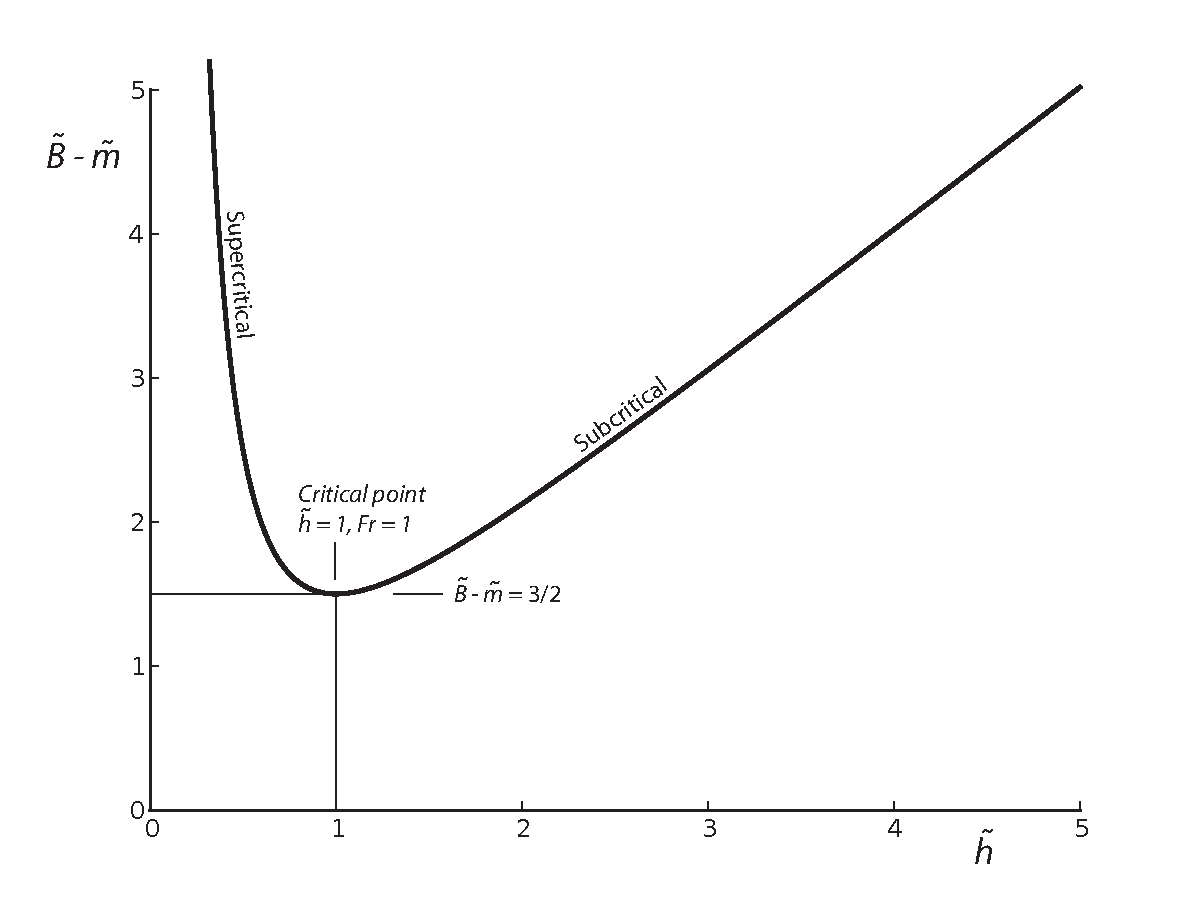
\includegraphics[width=5in]{hydraulic_B-m} 
    \caption{The normalized Bernouilli equation is plotted to show the normalized available head as a function of normalized fluid thickness.}
    \label{fig:hydraulic_B-m}
\end{figure}

The point defined by $Fr=1$ is called the {\it critical point}, separating \emph{subcritical} flow ($Fr < 1$) from the \emph{supercritical} flow ($Fr>1$) for the asymmetrical dam break problem.  This point also limits the transport possible for the asymmetric solution, since the the flow must pass through this point in the $\tilde{B}-\tilde{m}$ curve in the transition from subcritical to supercritical.  

For symmetric flows -- flows that are the same at $x=\pm\infty$ may be either subcritical or supercritical in the far field.  For subcritical flows, there will be a depression in sea surface elevation over a bump, for supercritical flows there will be a rise in sea surface elevation over a bump.  Asymmetric solutions require that the flow be exactly critical at the maximum constriction point, at the peak of the bump.  Thus, whereas the flow in the symmetric cases, with sub- or super-critical flow, the transport may be specified.  However, with the asymmetric case, the transport at the constriction point is determined by the critical condition.  We can calculate this by noting that, at the critical point, $\tilde{B} - \tilde{m} = \frac{3}{2}$.  Dimensionalizing shows that the elevation of the far field sea surface above the maximum obstacle height, $g H - g m$, is related to the transport, $Q$, by the equation
\begin{equation}
    H - m = \frac{3}{2} D = \frac{Q^{2/3}}{b^{2/3} g^{1/3}} \; .
\end{equation}

For a dam break problem, gravity waves will transfer the information of the water transport over the obstacle upstream, thereby setting the upstream transport.  If, on the other hand, the upstream transport is specified to be some value other than that required by critical flow at the constriction, part of the flow will be blocked, thereby raising the upstream head until the available head, and the transport over the sill are in balance.  Events that occur downstream of the critical point, on the supercritical side of the obstacle, have no influence on upstream conditions, as the supercritical flow does not allow gravity waves to propagate upstream.  Thus, the upstream side of the critical point is isolated from what occurs downstream.

If the downstream reservoir begins to fill, a \emph{hydraulic jump} may form, where the flow transitions back to subcritical.  This is a turbulent transition of the flow from supercritical to subcritical, often seen at the bottom of a weir, or as the ring that forms around the water flowing into a sink.  The water downstream of the hydraulic jump must meet or exceed the thickness of the subcritical branch associated with the supercritical flow in the $\tilde{B} - \tilde{m}$ curve, otherwise the jump with be advected downstream.  A thicker flow will create a hydraulic jump that propagates upstream.  Eventually, as in the case of water filling a sink that eventually fills with completely subcritical water, the control point is flooded, erasing the critical point.

% By vertically integrating the momentum equation (using the total pressure instead of sea level elevation),
% \begin{equation}
%     \frac{1}{2}u^2 + \frac{p}{\rho_0} = C
% \end{equation}
% where $C$ is constant, we find that
% \begin{equation}
%     \int_m^\eta \frac{1}{2}u^2 + \frac{p}{\rho_0} dz 
%     = C h 
%     = \frac{1}{2}\left( h u^2 + g \eta^2 - g m^2 \right)
% \end{equation}
% So that, using the relation $\eta = h + m$,
% \begin{equation}
%     u^2 + g h = g H - g m
% \end{equation}
% where, again $C = gH$, and $gH-gm$ is the available head in the region where $m$ is large, and $u \rightarrow 0$.
% 
% Downstream, the supercritical flow may also 

A very similar procedure used to calculate the solution with a bump on the seafloor may be used to calculate the solution width variations; the derivation in only outlined here. The following relationship defines the control point
\begin{equation}
    \frac{h_x}{h}(Fr^2 - 1) = \frac{b_x}{b}Fr^2.
\end{equation}
Bernouilli's equation is
\begin{equation}
    \frac{Q}{2 b^2} = Bh^2 - g h^3
\end{equation}
or, substituting $b=W\tilde{b}$, $h=D\tilde{h}$, and $m=D\tilde{m}$, where $D = 2^{-1/3} W^{2/3} Q^{2/3} g^{-1/3}$, the normalized relationship between width and fluid thickness is
\begin{equation}
    \tilde{b} = (\tilde{h}^2 - \tilde{h}^3)^{-1/2}
\end{equation}
Note, solutions are not defined for $\tilde{h} > 1$, \emph{i.e.}, $D$ is the maximum possible (dimensional) depth.

%%%%%% Add section on tides in estuaries.  Overtide, flood-vs-ebb dominant estuaries
%%%%%%  estuary shape (Friedrichs),



%%%%%%%%%%%%%%%%%%%%%%%%%%%%%%%%%%%%%%%%%%%%%%%%%%%%%%%%%%%%%%%%%%%%%%%%%%%%%%
%%%%%%%%%%%%%%%  BAROCLINIC FLOW CHAPTER  %%%%%%%%%%%%%%%%%%%%%%%%%%%%%%%%%%%%
%%%%%%%%%%%%%%%%%%%%%%%%%%%%%%%%%%%%%%%%%%%%%%%%%%%%%%%%%%%%%%%%%%%%%%%%%%%%%%

\chapter{Baroclinic Flow}

For the discussion of baroclinic flow, we will consider a slightly expanded set of governing equations.  We will ignore complexities in the equation of state, and either treat density as the primary water property, or relate either temperature or salinity to density through a linearized equation of state; that is, assume that $\rho=\rho_0 - \alpha T$ or $\rho=\rho_0 + \beta S$.  We will retain the vertical mixing term, since (turbulent) vertical mixing will be important for some examples, but ignore horizontal mixing, justified based on the very small aspect ratio of geophysical flows.  For the moment, we will treat the turbulent mixing of density and momentum as the same, both with turbulent mixing coefficient of $\kappa$.  Generally, we will assume that the flow is hydrostatic, with the notable exception of internal waves where the vertical acceleration is retained in some cases.  Also notice that the gravitational term now contains a variable density -- this is the only place in the momentum equations where density is not assumed to be constant, a consequence of the Bousinesq approximation.

\begin{align}
    \frac{\partial u}{\partial t} 
        + u\frac{\partial u}{\partial x} 
        + v\frac{\partial u}{\partial y} 
        + w\frac{\partial u}{\partial z} - fv 
                &= -\frac{1}{\rho_0}\frac{\partial p}{\partial x} 
                   +\frac{\partial}{\partial z}\left( 
                        \kappa \frac{\partial u}{\partial z}
                        \right) \label{eq:u-baroclinic} \\
    \frac{\partial v}{\partial t} 
        + u\frac{\partial v}{\partial x} 
        + v\frac{\partial v}{\partial y} 
        + w\frac{\partial v}{\partial z} + fu 
                &= -\frac{1}{\rho_0}\frac{\partial p}{\partial y}
                   +\frac{\partial}{\partial z}\left( 
                        \kappa \frac{\partial v}{\partial z}
                        \right)  \label{eq:v-baroclinic} \\
    \frac{\partial w}{\partial t}  
                &= -\frac{1}{\rho_0}\frac{\partial p}{\partial z} 
                   -\frac{g \rho}{\rho_0} \label{eq:w-baroclinic} \\
    \frac{\partial u}{\partial x} 
        + \frac{\partial v}{\partial y} 
        + \frac{\partial w}{\partial z} 
                &= 0 \label{eq:cont-baroclinic}\\
    \frac{\partial \rho}{\partial t} 
        + u\frac{\partial \rho}{\partial x} 
        + v\frac{\partial \rho}{\partial y} 
        + w\frac{\partial \rho}{\partial z}
                &= \frac{\partial}{\partial z}\left( 
                        \kappa \frac{\partial \rho}{\partial z}
                        \right)
\end{align}

These equations describe fully three-dimensional flow.  In order to obtain analytical solutions, we must restrict the dimensions of the problem somehow, for example, assuming that the density varies only depth, and is horizontally uniform.  In the next section, we will investigate the assumption that the stratification is confined to a thin layer that separates to relatively homogeneous water masses, a common occurrence in the ocean.  We will examine this case first because of the analogies that can be made to the barotropic flow in the previous chapter.  In short, if we consider a single, active, buoyant layer, we may replace gravity, $g$, with the reduced gravity, $g'$.  Thus, all of the barotropic models presented in the previous chapter have baroclinic layer-model counterparts.


\section{The reduced gravity layer model}

Consider a buoyant layer separated from a quiescent deep layer, both with constant density, see figure~\ref{fig:reduced_gravity_model}.  The density difference between the two layers is $\Delta\rho$.  If there is no motion in the lower layer, the horizontal pressure gradients there must be zero, otherwise a flow would be generated.  So, to calculate the pressure gradients in the upper layer, we will integrate the hydrostatic equation from some horizontal plane completely within the lower layer, $z=z_0$, through the interface, $z=-h$, up to the free surface, $z=\eta$.
\begin{equation}
    \int_{z_0}^{\eta} p_z \, dz = p_{\mathrm{ATM}} - p|_{z=z_0} = \int_{z_0}^{\eta} \rho g \, dz = 
        \rho_0 g (h - z_0) + (\rho_0-\Delta\rho) g (\eta - h) \;.
\end{equation}
Now, take a horizontal derivative of the equation, say in the $x$-direction, to get
\begin{equation}
     \rho_0 g h_x + (\rho_0-\Delta\rho) g (\eta_x - h_x) = 0 \; ,
\end{equation}
since
\begin{equation}
    \frac{\partial p_{\mathrm{ATM}}}{\partial x} = \frac{\partial p|_{z=z_0}}{\partial x} =
    \frac{\partial z_0}{\partial x} = 0 \; .
\end{equation}
Relating gradients in $\eta$ to gradients in $h$ gives,
\begin{equation}
    \frac{g \Delta\rho}{\rho_0} h_x = g \eta_x
\end{equation}
If we consider the reference free surface, $\eta = 0$, to be defined in a region without an active upper layer, the presence of buoyant water will elevate the free surface.  Because of the constraint that there is no motion in the lower layer, the interface thickness exactly mirrors the free surface, with a magnification proportional to $(\Delta\rho \rho_0^{-1})^{-1}$.  The mass deficit over the buoyant fluid, $\Delta\rho h$, must be equal to the mass surplus associated with the elevated free surface, $\rho_0 \eta$.  The deficit and surplus mass must exactly balance to ensure that there are no pressure gradients below the active layer.  The factor in front of the thickness gradients on the left hand side is refered to as the \emph{reduced gravity},
\begin{equation}
    g' = \frac{g \Delta\rho}{\rho_0}
\end{equation}
Thus, the only change that needs to be made for the momentum equations is to replace the pressure gradient term in $\eta$ with one defined with $h$.  The continuity equation relates changes in $h$ to the divergence in transport.  Thus, the inviscid, governing equations for the reduced gravity model are
\begin{align}
    u_t + u u_x + v u_y - f v &= -g' h_x \\
    v_t + u v_x + v v_y + fu &= -g' h_y  \\
    (u h)_x + (v h)_y &= -h_t
\end{align}

\begin{figure}[\begin{figure}[bt]
  \centering
    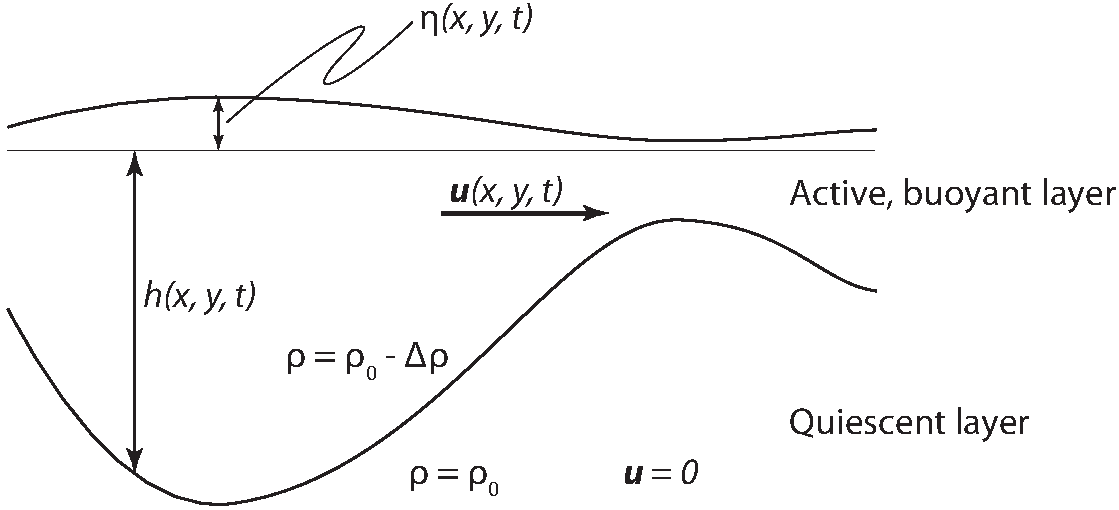
\includegraphics[width=5in]{reduced_gravity_variables.pdf}
    \caption{Variable definition for the reduced gravity model.}
  \label{fig:reduced_gravity_model}
\end{figure}

If the upper layer thickness is of nearly uniform thickness, $h = H + h'$, where $h' \ll H$, the continuity equation may be simplified as
\begin{equation}
    H u_x + H v_y = -h'_t
\end{equation}
and this set of equations is identical to the constant depth barotropic shallow water equations.  Thus, any of the constant depth barotropic shallow water models presented in Chapter~2 may be directly translated to a reduced gravity model by substituting $h'$ for $\eta$, and $g'$ for $g$.  The primary effect of this change is to reduce the deformation radius by a factor of $(\Delta\rho \rho_0^{-1})^{1/2}$.  Other dynamical properties remain identical.

One important feature of baroclinic flows, however, is frontal formation.  Frontal formation in a reduced gravity model requires that the interface contacts the surface; $h$ is non-zero where there is buoyant water, but approaches zero near the front.  In this case, it is not possible to assume that the upper layer thickness is approximately constant.  However, there are many properties of shallow water barotropic flow that carry over into a reduced gravity model with large amplitude depth changes.  To illustrate this, consider the adjustment problem of a buoyant layer, initially with thickness $H$, as shown in figure~\ref{fig:reduced_gravity_adjustment}.

\begin{figure}[bt]
    \centering
        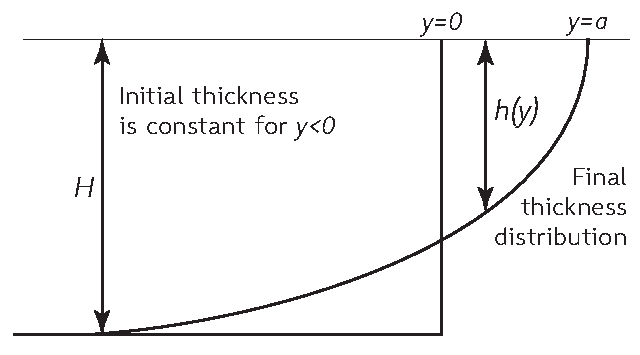
\includegraphics[height=2in]{reduced_gravity_adjustment.pdf}
    \caption{The initial and final condition for a reduced gravity adjustment problem, including the final position of the front at $y=a$.}
    \label{fig:reduced_gravity_adjustment}
\end{figure}

As in the other adjustment problems, this problem is grounded in the conservation of potential vorticity
\begin{equation}
    \frac{D}{Dt}\left(\frac{f + \zeta}{h}\right) = 0
\end{equation}
If we assume that the final state is steady and geostrophic, potential vorticity conservation requires that $\zeta = g' f^{-1} h_yy$.  Equating the potential vorticity of the initial and final states gives
\begin{equation}
    H - R_i^2 h_{yy} = h 
\end{equation}
where
\begin{equation}
    R_i^2 = \frac{\sqrt{g' H}}{f}
\end{equation}
is the internal deformation radius.  Homogeneous solutions are related to exponential growth and decay, with a the internal deformation radius defining the growth and decay scales; the particular solution is $h=H$.  Thus
\begin{equation}
    h = H + A e^{-y/R_i} + B e^{y/R_i}
\end{equation}
Clearly, $A=0$ if the solution is to remain bounded.  To determine $B$, we must calculate the final position of the front, $y=a$, which may have shifted from $y=0$ during the adjustment process.  Note that, at $y=a$, $h=0$, so
\begin{equation}
    \label{eq:reduced_gravity_adjustment_B_1}
    \frac{B}{H} = -e^{-a/Rd}
\end{equation}

Far from the initial front, we assume that the upper layer is unaffected by the adjustment process, similar to the barotropic adjustment solutions.  So, we know that the excess buoyant water found in the region $y>0$ must be balanced by a deficit in the $y<0$ region (the deficit is defined by $H-h$).  So, balancing integrals defining the excess and deficit, we get
\begin{equation}
    \int_{-\infty}^0 -B e^{y/R_i} \, dy = \int_0^a H + B e^{y/R_i}
\end{equation}
This has solutions defined by
\begin{equation}
    \label{eq:reduced_gravity_adjustment_B_2}
    \frac{B}{H} = - \frac{a}{R_i} e^{-a/R_i}
\end{equation}
Combining equations~\ref{eq:reduced_gravity_adjustment_B_1} and~\ref{eq:reduced_gravity_adjustment_B_2}, we find that $a = R_i$, and $B = -H e^{-1}$.  It is convenient to shift the solution, $\xi = y-a$, such that the adjusted front lies at $\xi = 0$; we find that
\begin{equation}
    h = H - H e^{\xi/R_i} \; .
\end{equation}

The flow speed at the adjusted front, $\xi = 0$, may be calculated by
\begin{equation}
    u = \frac{g'}{f} h_\xi = \sqrt{g' H} \; .
\end{equation}
Thus, the flow at the front is defined by critical flow, $Fr = 1$.  This does not depend on any of the model parameters, supercritical flow occurs along every front that is formed through this adjustment process.  So we expect that large-scale (geostrophic) fronts found in nature will typically be characterized by very energetic flow.

This kind of front is called a \emph{constant PV} solution, because the initial condition determines the potential vorticity for all of the buoyant fluid to be $f H^{-1}$.  It is also possible that a feature adjusts from an initial condition much deeper than the final thickness distribution.  In this case, it is possible to define a \emph{zero PV} solution, because as $H \rightarrow \infty$, $f H^{-1} \rightarrow 0$.  This class of solutions is explored further in problem~\ref{prob:zero_pv_eddy}.  Notice that such solutions are associated with very strong shear flows, since the assumption of zero potential vorticity requires that $\zeta = -f$.



\section{Baroclinic flow in a channel}

Consider a (non-rotating) channel that initially has a linear density gradient along the $x$-axis, the axis of the channel; the fluid is initially vertically uniform.  For this simple example, we will ignore the effects of both rotation and friction.  As rotation is ignored, we do not need to consider the cross-channel momentum equation, as the solution to that is trivial ($v=0$).  As we will see, the horizontal density gradients will cause an along-channel flow to form.  This flow will, in turn, cause the density field to evolve, and thus the horizontal advective term in the density equation ($u \rho_x$) must be retained.  The governing equations are then
\begin{align}
    \frac{\partial u}{\partial t} 
        &= -\frac{1}{\rho_0}\frac{\partial p}{\partial x} \label{eq:u-linear-channel} \\
    0  &= -\frac{1}{\rho_0}\frac{\partial p}{\partial z} 
                   -\frac{g \rho}{\rho_0} \label{eq:w-linear-channel} \\
    \frac{\partial u}{\partial x} &= 0 \label{eq:cont-linear-channel}\\
    \frac{\partial \rho}{\partial t} + u\frac{\partial \rho}{\partial x} &= 0 \label{eq:dens-linear-channel}
\end{align}
Vertically integrate equation~\ref{eq:w-linear-channel} from the surface ($z=\eta$) to some point in the water column, $z$, to get
\begin{equation}
    p_{\mathrm{ATM}} - p(z) = - \int_z^\eta \rho g\;dz
\end{equation}
The integral may be split into two parts
\begin{equation}
    p_{\mathrm{ATM}} - p(z) = - \int_0^\eta \rho g\;dz - \int_z^0 \rho g\;dz
\end{equation}
The first term on the right hand side will be the \emph{barotropic} pressure gradient, constant with depth through the fluid.  The second term is the \emph{baroclinic} pressure gradient that changes with depth.  

To simplify the representation of the barotripic pressure gradient, we can either assume that density changes from $z=0$ to $\eta$ are small, such that the density may be approximated as constant over this range so that integrand in the first term on the right hand side may be considered constant.  Or, we may assume a ridged lid so that sea level is set to be at $z=0$, and the barotropic pressure gradient is communicated through a pressure on the lid.  This may be accomplished in the above expression by assuming a pressure gradient in $p_{\mathrm{ATM}}$.  We will use the former assumption to get
\begin{equation}
    p = g \rho_0 \eta + \int_z^0 \rho g\;dz
\end{equation}
We require a lateral gradient of the pressure for substitution into the momentum equation~\ref{eq:u-linear-channel}.  However, in order for this to be analytically tractable, we need to assume that the lateral gradients of density are constant with depth, so the integral reduces to a manageable expression.  This is equivalent to assuming that the baroclinic pressure gradient changes linearly with depth.  This assumption -- used in many studies of estuarine dynamics -- places a strong constraint on the applicability of the solutions.  The horizontal pressure gradient, assuming $(\rho_x)_z = 0$, is then
\begin{equation}
    p_x = g \rho_0 \eta_x + \rho_x g z
\end{equation}
so that substitution into the momentum equation~\ref{eq:u-linear-channel} gives
\begin{equation}
    \label{eq:linear-channel-u_t}
    u_t =  -g \eta_x - \frac{\rho_x g}{\rho_0} z.
\end{equation}
Let us define the buoyancy,
\begin{equation}
    b = g\frac{\rho_0 - \rho}{\rho_0}
\end{equation}
so that
\begin{equation}
    \frac{\rho_x g}{\rho_0} = -b_x
\end{equation}
Equation~\ref{eq:dens-linear-channel} now becomes
\begin{equation}
    \label{eq:linear-channel-buoyancy}
    b_t + u b_x = 0.
\end{equation}
As $b_x$ is initially constant, and there is no vertical flow that could change this, $b_x$ may be considered to be constant at all times.  This means that $b_{xt} = 0$.  Thus, taking a derivative with respect to time gives
\begin{equation}
    b_tt + u_t b_x = 0.
\end{equation}
Combining this with equation~\ref{eq:linear-channel-u_t} gives
\begin{equation}
    b_{tt} = g b_x \eta_x - (b_x)^2 z
\end{equation}
Since $b_x$ is constant in time, so must $\eta_x$ also be constant in time.  Integration with respect to time, then gives
\begin{equation}
    \label{eq:linear-channel-b}
    b_t = g b_x \eta_x t - (b_x)^2 z t + C
\end{equation}
where $C$ is an integration constant, possibly dependent on $z$.  Note that by vertically integrating equation~\ref{eq:linear-channel-buoyancy},
\begin{equation}
    \frac{\partial}{\partial t} \int_{-H}^\eta b\;dz = - b_x \int_{-H}^\eta u\;dz
\end{equation}
So, if we set the mean flow in the channel to zero, the vertical mean density remains constant in time.  Note, we could set the mean flow to be non-zero, but this would just shift the entire density structure with the flow.  So, setting the vertical mean flow to zero does not fundamentally alter the solution, and it is much easier to deal with.

Vertically integrating equation~\ref{eq:linear-channel-b} gives
\begin{equation}
    \int_{-H}^\eta b_t\;dz = g \eta_x b_x H - \frac{1}{2}(b_x)^2 H^2 t + \bar{C} H = 0
\end{equation}
where $\bar{C}$ is the vertical mean of $C$ -- we don't care about the vertical structure of $C$, just the mean value $\bar{C}$.  Solving for $\bar{C}$, we find
\begin{equation}
    \bar{C} = -g \eta_x b_x + \frac{1}{2} (b_x)^2 H t
\end{equation}
and
\begin{equation}
    b_t = (b_x)^2 t \left( \frac{H}{2} - z \right)
\end{equation}
Integrating in time gives the final solution for the evolution of the density field
\begin{equation}
    b = \frac{1}{2}(b_x)^2 t^2 \left( \frac{H}{2} - z \right) + B_I
\end{equation}
where $B_I$ is the initial condition at $t=0$.  For the case we are considering, there are initialy no vertical gradients of buoyancy or density, so $B_{Iz} = 0$.  Now, we can solve for the along-channel flow structure, $u$,
\begin{equation}
    u = \frac{-b_t}{b_x} = \frac{(b_x)^2 t \left( \frac{H}{2} - z \right)}{b_x}
         = b_x t \left( \frac{H}{2} - z \right)
\end{equation}

An interesting feature of this solution is that the Richardson number does not change in time.  The Richardson number is defined as
\begin{equation}
    Ri = \frac{N^2}{S^2} = \frac{b_z}{(u_z)^2}.
\end{equation}
We know from our solution that $b_z = \frac{1}{2}(b_x)^2 t^2$, and $(u_z)^2 = (b_x)^2 t^2$, so that $Ri=\frac{1}{2}$ at all times.  The flow is always stable, since the Richardson number is always larger than $\frac{1}{4}$.  This may seem curious since the flow is constantly accelerating.  However, the vertical density gradients are also always increasing, such that the effects of increased shear and increased stratification cancel each other out.



\section{Estuarine circulation}

The simplest model of estuarine circulation may be derived by combining a mass balance, equating the inflow ($Q_{in}$) and outflow ($Q_{out}$) at the estuary mouth with the river flow ($Q_R$),
\begin{equation}
    Q_{in} + Q_R = Q_{out} \; ,
\end{equation}
and a salt balance, noting that since the river salinity is zero, the net salt flux at the estuary mouth due to the exchange flow must vanish
\begin{equation}
    S_{in} Q_{in} = S_{out} Q_{out} \; .
\end{equation}
Eliminating $Q_{in}$, and rearranging gives
\begin{equation}
    Q_{out} = Q_R \left( \frac{\Delta S}{S_{out}} \right)^{-1}
\end{equation}
where $\Delta S = S_{in} - S_{out}$.  This relationship is called Knudsen's relation \citep{knudsen:00}, and it relates the estuarine outflow to the river discharge and stratification at the mouth.  Notice that the stratification at the mouth is a robust quantity, as it is related to the net mixing within the entire estuary, rather than the mean exchange flow at the mouth, which may be obfuscated by the tides.  Stratification at the mouth also sets the density anomaly for the river plume that forms from the estuarine outflow.  However, this equation is diagnostic in that the stratification at the estuary mouth must be known in order to calculate the magnitude of the exchange flow; Knudsen's relation cannot be used to predict $\Delta S$.

In order to predict both the stratification and estuarine exchange flow at the estuary mouth, a momentum balance must be added to the conservation of mass and salt. The following outlines an heuristic derivation of scales in estuarine circulation.  The solution assumes that the estuarine circulation is a balance between gravitationally-driven exchange flow and vertical mixing.  The full solution, originally derived by \citet{hansen.rattray:65} and \citet{chatwin:76}, has recently reviewed in a publication by \citet{maccready.geyer:10}.

The relevant tidally-averaged equations assume steady flow, and constant vertical eddy diffusivity, $\kappa_\rho$, and viscosity, $\kappa_u$, caused by tidal mixing.  Also, we will assume a simplified equation of state, $\rho = \rho_0 + \beta S$, the salinity, $S$, is the only factor that determines density.
\begin{align}
    0 = -\frac{1}{\rho_0}\frac{\partial p}{\partial x} + \kappa_u \frac{\partial^2 u}{\partial z^2}
        \label{eq:est_hmoment} \\
    0 =  -\frac{1}{\rho_0}\frac{\partial p}{\partial z} - g\frac{\rho_0 + \beta S}{\rho_0}
        \label{eq:est_vmoment} \\
    u\frac{\partial S}{\partial x} = \kappa_\rho \frac{\partial^2 S}{\partial z^2}
        \label{eq:est_salt_cons}
\end{align}

Just as in the previous section, we must assume that $(S_x)_z = 0$, \emph{i.e.}, that the along-channel salinity gradient is constant with depth.  This means that we will exclude \emph{salt wedge} estuaries from consideration, as they have large horizontal salinity gradients in the lower layer, in the vicinity of the nose of the salt intrusion, but very small horizontal salinity gradients in the upper layer where the water is nearly fresh along the entire estuary.  Thus, we are considering a class of estuaries referred to as \emph{partially mixed}.  

Eliminate pressure from the two momentum equations, \ref{eq:est_hmoment} and \ref{eq:est_vmoment}, by cross-differentiation to get
\begin{equation}
    0 = \kappa_u \frac{\partial^3 u}{\partial z^3} + \frac{g \beta}{\rho_0}\frac{\partial S}{\partial x} \; .     \label{eq:est_moments}
\end{equation}
Note that the second term is constant with respect to $z$, by our assumption that $S_x$ is constant with depth.  This means that we have polynomial-type solutions for the vertical flow profile.  The salt conservation equation~\ref{eq:est_salt_cons} then implies that the salinity profile also has a polynomial form.

Now, let us consider three characteristic scales of the estuarine circulation: the length scale of the salt intrusion into the estuary, $L \sim S_0 (S_x)^{-1}$, where $S_0$ is the oceanic salinity at the estuary mouth; the vertical stratification, $\Delta S \sim H S_z$, where $H$ is the characteristic depth of the estuary; and the vertical shear in the horizontal flow, $\Delta u \sim H u_z$.  Applying these scales to equation~\ref{eq:est_moments} gives
\begin{equation}
    \Delta u \sim \frac{g S_0 \beta H^3}{L \kappa_u \rho_0} \; .
    \label{eq:est_deltau}
\end{equation}
Scaling the \emph{local} salt balance, equation~\ref{eq:est_salt_cons}, gives
\begin{equation}
    \Delta S \sim \frac{S_0 H^2}{\kappa_\rho L} \Delta u 
             = \frac{g \beta S_0^2 H^5}{\kappa_{\rho} \kappa_u \rho_0 L^2}
    \label{eq:est_deltas}
\end{equation}

We will treat the estuarine circulation separately from the mean flow associated with the river transport.  The estuarine circulation will have a vertical integral of zero, and will flow riverward in the lower layer, $u_{lower}$ and seaward at the surface, $u_{surface}$, so that here $u_{lower} + u_{upper} = 0$.  If the water column is stratified, i.e., $s_{lower} > s_{upper}$, this creates a net up-estuary salt flux, since $u_{lower} s_{lower} > u_{upper} s_{upper}$.  The up-estuary salt flux can be scaled as $\Delta u \Delta s$.  For the estuary to remain in a steady state, this up estuary salt flux generated by the estuarine circulation must be balanced by a down estuary salt flux associated with the river flow, $u_R S_0$.  Thus, the \emph{global} salt balance is
\begin{equation}
    \Delta u \Delta S = u_R S_0
\end{equation}
We can use this equation to combine equations~\ref{eq:est_deltau} and \ref{eq:est_deltas}, to get an equation for the scale of the horizontal estuarine salt intrusion length scale
\begin{equation}
    L \sim \frac{g^{2/3} \beta^{2/3} S_0^{2/3} H^{8/3}}{u_R^{1/3} \rho_0^{2/3} \kappa_u^{2/3} \kappa_\rho^{1/3} }
\end{equation}
A few terms appear in this equation that are very useful in describing estuarine circulation.  First of all, we may define
\begin{equation}
    g'_f = \frac{g \beta S_0}{\rho_0},
\end{equation}
the reduced gravity associated with the density difference between purely fresh and purely oceanic water ($\Delta rho_f \sim \beta S_0s$), \emph{i.e.}, the reduced gravity associated with the greatest density differences possible in the system.  This may be used to define the \emph{fresh water Froude number},
\begin{equation}
    Fr_f = \frac{u_R}{\sqrt{g'_f H}}.
\end{equation}
This is the smallest possible Froude number supported by the system because $g'_f$ is the largest possible value of $g'$ possible, $H$ is the largest possible vertical length scale, and $u_R$ is the smallest velocity scale (the velocity scale if the exchange flow, $\Delta u$, is zero; a non-zero exchange flow increases the scale of the absolute velocity, $u_R + \Delta u$).  

Thus, the horizontal estuarine salt intrusion length scale becomes
\begin{equation}
    L \sim \frac{u_R}{Fr_f^{4/3}} \frac{H^2}{\kappa_u^{2/3} \kappa_\rho^{1/3}}
\end{equation}
which may in turn be used to define the two vertical scales
\begin{align}
    \Delta u &\sim \frac{u_R^2}{Fr_f^2}\frac{H^2}{\kappa_u L} 
         = \frac{u_R}{Fr_f^{2/3}} \left( \frac{\kappa_\rho}{\kappa_u} \right)^{1/3} \; ,\\
    \Delta S &\sim \frac{u_R^2}{Fr_f^2}\frac{S_0\,H^4}{\kappa_u \kappa_\rho L^2} 
         =  S_0\,Fr_f^{2/3} \left( \frac{\kappa_u}{\kappa_\rho} \right)^{1/3} \; .
\end{align}
The full solutions for $u$ and $S$ are polynomials in the $z$-direction, proportional to $\Delta u$ and $Delta S$, with possibly large constant numerical multipliers.  For example, the full solution for $S$ is an $\mathcal{O}(1)$ polynomial multiplied $48 \Delta S$.  

There are a number of interesting and surprising aspects to the parameter dependencies of the estuarine scales.  For the following discussion, we will assume that the Prandlt number, $Pr = \kappa_u / \kappa_\rho$, is $\mathcal{O}(1)$, so that $\kappa_u \sim \kappa_\rho \sim \kappa$.  In this case, both the magnitude of the estuarine exchange flow, $\Delta u$, and the vertical stratification, $\Delta S$, are independent of vertical mixing.  This is surprising, because we expect that as mixing increases, both stratification and shear will decrease.  At the same time, the estuarine salt intrusion length scale, $L$, depends inversely on the vertical mixing coefficient, $\kappa$.

The inverse relationship between intrusion length scale and vertical mixing may be explained by considering the flow in the lower layer entering the estuary at the mouth.  If the exchange flow and vertical stratification remain constant, the salt will be able to enter the upper layer (and be exported from the estuary) twice as quickly if the vertical mixing is twice as strong, thus halving the required length scale of the estuary.  The independence of the exchange flow on vertical mixing may be explained by examining the force balance causing the exchange flow.  If the mixing is doubled, viscosity will tend to reduce the exchange flow by half.  However, at the same time, the doubled vertical mixing will halve the intrusion length scale, doubling the horizontal pressure gradient, and doubling the gravitational exchange flow.  Thus, the tendency to decrease the exchange flow due to increased viscosity, and increase the exchange flow due to a larger baroclinic pressure gradient cancel each other out.

The estuary scales also depend on the magnitude of the river flow.  Note that, if $S_0$ is constant, $Fr_f$ is proportional to $u_R$, so that the dependence of the estuarine scales to $u_R$ is
\begin{equation}
    L \propto u_R^{-1/3} \; , \qquad \Delta u \propto u_R^{1/3} \;, \qquad \mathrm{and} \qquad \Delta S \propto u_R^{2/3}   \;.
\end{equation}
These scales are all as expected.  The estuarine salt flux $\Delta u \Delta S$ must increase in proportion to $u_R S_0$.  And although the increased exchange flow acts to increase the intrusion length scale (proportional to $u_R^{1/3}$), the increased stratification increases the effectiveness of the (constant) vertical mixing even more, proportional to $u_R^{2/3}$, with a tendency to reduce the intrusion length scale.  Thus, although the lower layer flow is increased, it looses salt even more rapidly through vertical diffusion, in the balance reducing the intrusion length scale by $u_R^{-1/3}$.

% Problems with basic estuarine circulation theory
%, although this balance has been recently called into question by \citet{burchard.hetland:10}

% \section{Two-layer hydraulic control and overmixing}



\section{Internal waves}

Consider a ball of density $\rho_0$ in a uniformly stratified fluid, see figure~\ref{fig:stratified_ball}.  If the ball is displaced by some distance, $\Delta z$, there will be a force on the ball proportional to the density difference between the ball and the local surrounding fluid.  This force will be directed downward if the ball is moved up, and upward if the ball is moved down.  Now, we can use $F=m a$ to estimate the motion of the displaced ball.  Note that the Bousinesq approximation allows us to only consider density differences when multiplied by gravity, so that the mass times acceleration term is $\ddot{\Delta z} \rho_0$, where the dots denote time differentiation.  Thus
\begin{equation}
    g \rho_z \Delta{}z = \ddot{\Delta z} \rho_0
\end{equation}
which has solutions
\begin{equation}
    \Delta{}z = \Delta{}z_0 \,\mathrm{cos}(N t)
\end{equation}
where
\begin{equation}
    N =  \sqrt{ - \frac{g \rho_z}{\rho_0}}.
\end{equation}
Note, periodic solutions are only possible for real values of $N$, which requires $\rho_z<0$, or stable stratification with light water above heavy water.  We refer to $N$ as the \emph{stratification frequency}, since it is the natural frequency of motions in stratified flow.  Also, note here that the vertical acceleration is critical to the wave motions, so that the hydrostatic approximation cannot generally be made for all internal waves.  (However, it may be shown that the hydrostatic approximation is valid for very long waves, as we will see below.) Also, we need to consider how the density field will evolve -- for waves in the ocean it is the water itself that must be displaced upward, not just a ball.  Thus, we also need to retain the vertical advection term in the density equation. 

\begin{figure}
    \centering
    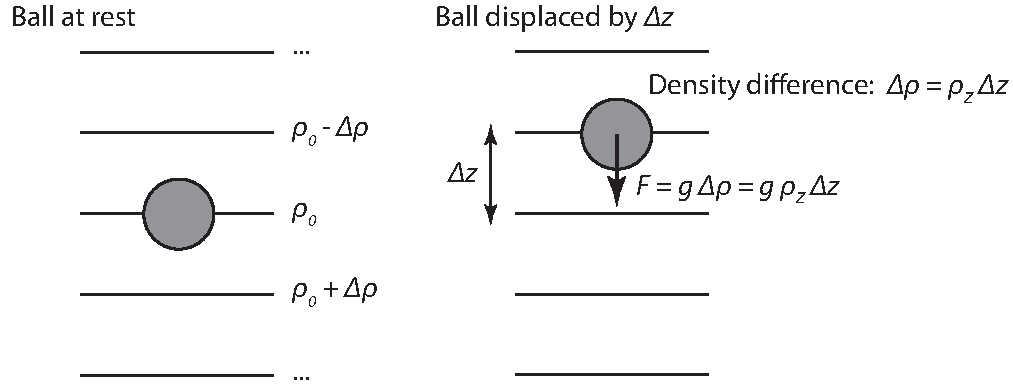
\includegraphics[width=4in]{stratified_ball}
    \label{fig:stratified_ball}
    \caption{Diagram showing the initial state of a ball with density $\rho_0$ at rest, and in a perturbed state.  The force on the ball is proportional to the local density difference between the ball and the fluid.}
\end{figure}

To examine inviscid waves in a uniformly stratified, rotating fluid, consider the linearized set of equations
\begin{align}
    \frac{\partial u}{\partial t} - fv 
        &= -\frac{1}{\rho_0}\frac{\partial p}{\partial x} \label{eq:u-linear-baroclinic} \\
    \frac{\partial v}{\partial t} + fu 
        &= -\frac{1}{\rho_0}\frac{\partial p}{\partial y} \label{eq:v-linear-baroclinic} \\
    \frac{\partial w}{\partial t}  
                &= -\frac{1}{\rho_0}\frac{\partial p}{\partial z} 
                   -\frac{g \rho'}{\rho_0} \label{eq:w-linear-baroclinic} \\
    \frac{\partial u}{\partial x} 
        + \frac{\partial v}{\partial y} 
        + \frac{\partial w}{\partial z} 
                &= 0 \label{eq:cont-linear-baroclinic}\\
    \frac{\partial \rho'}{\partial t} + w\frac{\partial \bar{\rho}}{\partial z}
                &= 0 \label{eq:dens-linear-baroclinic}
\end{align}
A key assumption is that $\rho = \rho_0 + \bar{\rho}(z) + \rho'(x, y, z, t)$, where $\rho_0 \gg \bar{\rho} \gg \rho'$.  This allows the vertical gradient of density in equation~\ref{eq:dens-linear-baroclinic} to be defined using the ambient stratification associated with $N^2$ with the relationship
\begin{equation}
    \frac{\partial \rho}{\partial z} \simeq \frac{\partial \bar{\rho}}{\partial z} = -\frac{N^2 \rho_0}{g} \; .
\end{equation}
As this is the only occurrence of a vertical density gradient, this is the only place that $N^2$ is found in the equations.  Where gradients of density other than in the $z$-direction occur, $\rho'$ is the only term left over.  In the vertical momentum equation, a reference pressure defined by
\begin{equation}
    \frac{\partial p}{\partial z} = -g (\rho_0 + \bar{\rho})
\end{equation}
is subtracted from the full hydrostatic equation, leaving the remainder term, $g \rho' \rho_0^{-1}$.

To solve this set of equations, we will assume a wave-like form for all variables
\begin{equation}
    \phi = \phi_* e^{i(kx+ly+mz-\omega{}t)} \; ,
\end{equation}
and substitute this into equations~\ref{eq:u-linear-baroclinic} through~\ref{eq:cont-linear-baroclinic}.  We then have a set of five linear equations, which we may solve by rearanging into the form $\mathrm{\mathbf{A}} \mathbf{x} = 0$, or
\begin{equation}
    \left[
    \begin{array}{ccccc}
         -i \omega & -f & 0 & i \,k\, \rho_0^{-1} & 0 \\
         f & -i \omega & 0 & i \,l\, \rho_0^{-1} &  0 \\
         0 & 0 & -i \omega & i \,m\, \rho_0^{-1} & g \rho_0^{-1} \\
         k & l & m & 0 & 0 \\
         0 & 0 & -\rho_0 N^2 g^{-1} & 0 & -i \omega
    \end{array}
    \right]
    \left(
    \begin{array}{c}
        u_* \\ v_* \\ w_* \\ p_* \\ \rho'_*
    \end{array}
    \right) = 0
\end{equation}
Non-trivial solutions only exist for $\mathrm{det}(\mathrm{\mathbf{A}})=0$, or
\begin{equation}
    m^2 (f^2 - \omega^2) + (k^2 + l^2)(N^2-\omega^2) = 0.
\end{equation}
Defining $\mathbf{k}^2 = k^2 + l^2 + m^2$ as the magnitude of the wavenumber vector, and $\mathbf{k_H}^2 = k^2 + l^2$ as the magnitude of the horizontal component of the wavenumber vector, we can define the wave frequency, $\omega$, in terms of the angle, $\theta$ between $\mathbf{k}$ and $\mathbf{k_H}$,
\begin{equation}
    \omega^2 = f^2 \mathrm{sin}^2\theta + N^2 \mathrm{cos}^2\theta .
\end{equation}
Thus, $\theta = 0$ is a purely horizontally propagating wave, $\theta = \pi / 2$ is a purely vertically propagating wave.  The group speed is defined by the gradient of $\omega$ with respect to the wavenumber, $\mathbf{c_g} = \nabla_k w$, so that each component is
\begin{align}
    c_{gx} &= \frac{\partial \omega}{\partial k}
           = +k \,\frac{m^2}{\mathbf{k}^4 \omega}(N^2-f^2)\\
    c_{gy} &= \frac{\partial \omega}{\partial k}
           = +l \,\frac{m^2}{\mathbf{k}^4 \omega}(N^2-f^2)\\
    c_{gz} &= \frac{\partial \omega}{\partial m}
           = -m \,\frac{\mathbf{k_H}^2 }{\mathbf{k}^4 \omega}(N^2 - f^2)
\end{align}

An interesting property of internal waves is that the group velocity vector is directed such that when the phase speed is upwards, $m>0$, the group velocity is upward, $c_{gz}<0$, and \emph{vica verse}.  Recall that the direction of phase propagation is determined by $\mathbf{k}$, whereas the direction of energy propagation is determined by $\mathbf{c_g}$\footnote{See \citet{cushman-roisin.beckers:11}, Appendix B for an excellent review of wave properties.}.  Since it may be easily demonstrated that $k\cdot\mathbf{c_g} = 0$, we also know that energy propagates in a direction perpendicular to the phase propagation.

Waves are approximately hydrostatic when the horizontal wavelength is much larger than the vertical wavelength, that is when $k^2, l^2 \ll m^2$ so that $\mathbf{k}^2 \simeq m^2$.  In other words, the angle $\theta$ is very close to zero.

% Of particular interest to coastal oceanography, however, is the idea of a critical slope.  

% Internal tides

% Solitons

% G-M spectrum ?

%%%%%%% ADD discussion on critical bathymetric slopes.

%%%%%% long waves dw/dt term is small -- only needed for short waves...



\section{Coastally-trapped waves}

At much larger scales, periodic motions in stratified flow over a continental shelf are explained by a process referred to as \emph{coastally-trapped waves}.  For historical reasons, barotropic motions are referred to as \emph{continental shelf waves}, and baroclinic motions are referred to as coastally-trapped waves.  Coastally-trapped wave theory can be very complicated, by including effects such as bottom friction, or considering possibly short waves.  Here, we will examine a simplified subset of the solution space, considering an inviscid solution with only very long waves ($\partial_x \rightarrow 0$).  We will also only consider free waves, with the understanding that the forced wave problem is similar to the coastally trapped waves, where the wind forcing excites various shelf wave modes that propagate at different speeds.

\begin{figure}[t]
    \centering
        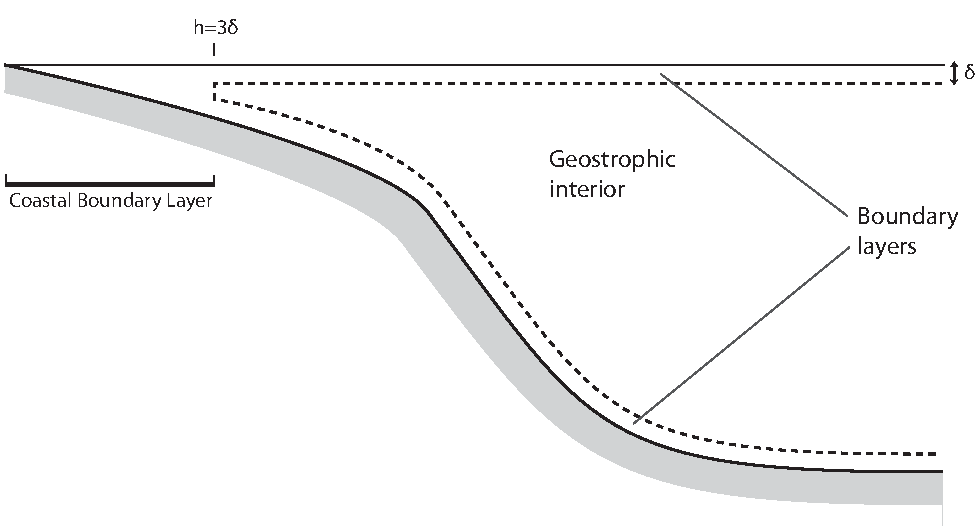
\includegraphics[height=3in]{shelf_cross-section.pdf}
    \caption{}
    \label{fig:shelf_cross-section}
\end{figure}

\begin{align}
    - i \omega u - fv &= 0 \label{eq:csw_xmoment}\\
    fu &= -\frac{1}{\rho_0}\frac{\partial p}{\partial y} \label{eq:csw_ymoment}\\
    0 &= -\frac{1}{\rho_0}\frac{\partial p}{\partial x} - \frac{g \rho'}{\rho_0} \label{eq:csw_hydrostatic}\\
    \frac{\partial v}{\partial y} + \frac{\partial w}{\partial z} &= 0 \label{eq:csw_continuity}\\
    -i \omega \rho' - w\frac{N^2 \rho_0}{g} &= 0 \label{eq:csw_density}
\end{align}
Again, as in the derivation of internal waves, we assume that $\rho = \rho_0 + \bar{\rho}(z) + \rho'(x, y, z, t)$, where $\rho_0 \gg \bar{\rho} \gg \rho'$, allowing the $\rho_z$ term to be replaced with a term containing the ambient stratification, $N^2$.  We will assume, again, as in the Kelvin wave and continental shelf wave discussions that the cross-shore balance is geostrophic, and that the along-shore wind stress is the primary driver of shelf circulation.  These assumptions require that timescales are much longer than $f^{-1}$, $\omega \ll f$, and that the motions are periodic in time, such that $\partial_t = -i \omega$ Also,the along-shore scales are again much, much longer than cross-shore scales, $L_x \gg L_y$.

We will combine the two momentum equations, \ref{eq:csw_xmoment} and \ref{eq:csw_ymoment}, to get an equation for $v$ in terms of pressure,
\begin{equation}
    v = \frac{i \omega p_y}{f^2 \rho_0} \; .
\end{equation}
An equation in $w$ may be found by combining the hydrostatic and density equations (\ref{eq:csw_hydrostatic} and \ref{eq:csw_density}) to get
\begin{equation}
    w = \frac{i \omega p_z}{N^2 \rho_0}
\end{equation}
Plugging the two relationships for $v$ and $w$ into the continuity equation yields the field equation
\begin{equation}
    p_{yy} + f^2 \left( \frac{p_z}{N^2} \right)_z = 0
\end{equation}
The boundary conditions are that the along-shore flow vanishes far from the coast, so
\begin{equation}
    p_y\bigg|_{y=\infty} = 0
\end{equation}
At the coast, the normal flow must vanish (note, that this is equivalent to vanishing along-shore flow at the coast as well -- an unrealistic aspect of the problem that can be mitigated by including friction),
\begin{equation}
    p_y\bigg|_{y=0} = 0
\end{equation}
At the surface, we will assume that divergence is small, as in the coastally-trapped wave problem, so the free surface acts as a ridged lid, with $w=0$, so that
\begin{equation}
    p_z\bigg|_{z=0} = 0
\end{equation}
At the bottom, the flow is directed along the sea floor; the vertical velocity must be equal to the cross-shore velocity times the bottom slope, or
\begin{equation}
    w\bigg|_{z=-h} + v h_y = 0
\end{equation}
or
\begin{equation}
    p_z\bigg|_{z=-h} = - \frac{N^2}{f^2} p_y h_y \; .
\end{equation}




\section{River plumes}

Here, four dynamical regions within a river plume are defined, the near-field, mid-field, far-field, and very far field, each progressing further from the estuary mouth.

\paragraph{Near-field}
A near-field plume may occur at the mouth of a narrow estuary.  The near-field plume is a region of very strong flow associated with rapid spreading of the plume and very intense mixing \citep{hetland:10a, nash.ea:09, macdonald.geyer:04}.  The near-field plume is characterized by a single, active layer of fresh water above a layer of more quiescent saline coastal water.  The plume is typically thin, ranging from less than a meter to a few meters in thickness, and there can be strong current shear or stratification within the plume.  The near-field plume exists only within a few kilometers from the estuary mouth before deceleration due to mixing, or turning due to the earth's rotation halt its rapid intrusion into the coastal ocean.  The near-field plume is often either modulated by the tides, or in the case where there is a reversal in the tidal flow at the estuary mouth, the near-field plume is discharged in tidal pulses.  Because of the rapid flow speeds, and relatively small size of the near-field plume, residence times of fresh water within this region are typically on the order of only a few hours.

The flow in the near-field is supercritical \citep[see, e.g.,][]{armi.farmer:86}, meaning that flow has speeds faster than the first-mode baroclinic wave speed, i.e., interfacial waves on the pycnocline between the plume and the ambient shelf water.  In other words, the flow is so fast that waves cannot propagate upstream.  The elevated shear associated with the rapidly moving plume water triggers shear instabilities \citep{ivey.imberger:91, macdonald.geyer:05}.

\citet{hetland:10} describes the interaction between lateral spreading and vertical mixing in the near-field plume.  Once the brackish estuarine water leaves the confines of the estuary channel, the water will spread laterally upon entering the coastal ocean.  By conservation of the water volume, the lateral spreading requires the base of the plume to shoal.  This shoaling is in turn associated with a drop in the sea level, and thus a drop in pressure.  By the Bernoulli principal, a drop in pressure corresponds to an acceleration of the flow, which enhances the vertical shear and the associated vertical mixing.  Thus, there is a competition between the spreading, which tends to accelerate the plume, and mixing which tends to decelerate the plume.  Initially, spreading dominates, and the plume experiences net acceleration as it enters the coastal ocean.  Ultimately, though, mixing dominates, and the plume eventually decelerates enough such that it is no longer a jet-like feature, but rather a plume-like feature.


A simple layer model is developed that includes plume spreading and entrainment.  The plume is assumed to be in a steady state and to have separated from the coast at the estuary mouth.  Plume spreading beyond the mouth results in a pie-shaped near-field plume region, as shown in the layer model setup (Figure~\ref{fig:layer_model_setup}).  \citet{hetland.macdonald:08} show that properties within the plume are a function of radial distance from the mouth (although for convenience, distance along the plume centerline is used here as the independent variable).  Thus,  plume width can be defined as the distance between two streamlines bracketing the core of the near-field plume, and the properties within these streamlines may be approximated as constant.

A buoyant fluid is introduced into a reservoir through a rectangular gap in a coastal wall with a width $W_0$, representing an estuary mouth.  The estuarine outflow is steady, with a velocity $u_0$ and density anomaly $\Delta\rho_0$ at the point where the flow enters the coastal ocean.  The quiescent ambient water in the coastal ocean has a uniform density, $\rho_0$.  The axes are oriented such that the origin is located at the center of the gap, with positive $x$ directed seaward from the source.  After the flow enters the ocean, it separates from the coast, spreads, thins, and entrains background water.

The notion of hydraulic control at the estuary mouth dates back to Stommel and Farmer's (1953) overmixing theory, later formalized and extended by \citet{armi.farmer:86}.\nocite{stommel.farmer:53}  Based on these theoretical studies and observations, the mouth is assumed to act as a constriction, and the flow is assumed to be exactly critical at the estuary mouth where the flow enters the ocean. Thus, the vertical thickness of the outflow at the estuary mouth, $h_0$, is specified such that the Froude number at $x=0$ is one, 

\begin{equation}
Fr\bigg|_{x=0}\equiv \frac{u_0}{\sqrt{g_0' h_0}} = 1, \label{eq:ic}
\end{equation}
where $g_0' \equiv g \Delta\rho_0 / \rho_0$ is the reduced gravity of the flow at the estuary mouth.  (Values at the boundary condition location $x=0$ are noted by a subscript $0$ throughout.)  This condition may be extended to include source water with a Froude number greater than one.  All of the results remain valid, but the functional dependencies described then also need to include the parameter $Fr_0 = Fr(x=0)$.

Continuity and density conservation may be used to relate the local flux of water at some point away from the coast to these constant estuary outflow properties,

\begin{equation}
Q \Delta\rho = h\,u\,W\,\Delta\rho = h_0\,u_0\,W_0\,\Delta\rho_0 = Q_0 \Delta\rho_0, \label{eq:mass}
\end{equation}
where $h$ is the active upper-layer thickness, $u$ the upper-layer radial velocity away from the estuary mouth, $\Delta\rho$ the density anomaly of the upper layer, and $Q_0$ is the volume flux leaving the estuary.  When entrainment is included, the local mass flux of the plume, $Q$, will increase away from the source.

\begin{figure}[htbp]
    \centering
        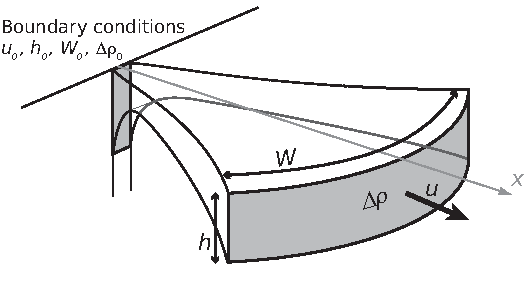
\includegraphics[height=3in]{layer_model_setup.pdf}
    \caption{Near-field layer model setup.}
    \label{fig:layer_model_setup}
\end{figure}

Assuming a steady state enables replacing the total derivative with a local advection term,

\begin{equation}
\frac{\mathrm{D}}{\mathrm{D} t} = u\frac{\partial}{\partial x},
\end{equation}
so that conservation of density and momentum in a non-rotating buoyant layer are

\begin{align}
u \frac{\partial \rho}{\partial x} &= \frac{w_e\,\Delta\rho}{h}, \label{eq:moment_full}\\
u \frac{\partial u}{\partial x} &=  -g' \frac{\partial h}{\partial x} - h \frac{\partial g'}{\partial x}- \frac{w_e\,u}{h}, \label{eq:density_full}
\end{align}
where $g' \equiv g \Delta\rho / \rho_0$ is the (variable) reduced gravity, and $w_e$ is an entrainment velocity.  Note that it is important to include the contribution of the variable density field to the pressure gradient, as the density of the outflow will change in the $x$-direction.  

An entrainment velocity, $w_e$, is defined to represent mixing of density and momentum from the lower layer into the upper layer.  There are a number of ways to define the entrainment velocity, often based on the internal, densimetric Froude number \citep[e.g.,][]{ellison.turner:59, turner:73, cenedese.ea:04}.  Although many different entrainment parameterizations were investigated, the results presented here use a constant entrainment rate, $\delta = w_e/u$.  This approximation is often used in engineering scale plumes, simplifies the mathematics, is consistent with $Fr$ = $\mathcal{O}(1)$, and produces a plume density structure similar to the three-dimensional model.  

In classic models of hydraulic flow, width is specified so that the problem has a single independent variable, oriented along-channel \citep[see][]{armi.farmer:86,turner:73,baines:95}.  Here, the width of the near-field plume is a variable that must be solved.  Previous studies \citep{wright.coleman:71, hetland.macdonald:08} have shown that the separated plume spreads perpendicular to the flow direction with a rate proportional to the local internal gravity wave speed, $c = \sqrt{g' h}$.  Thus, following a parcel of water, the local rate of change in plume width, $W$, is

\begin{equation}
\frac{\mathrm{D} W}{\mathrm{D} t} = u \frac{\partial W}{\partial x} = 2 \sqrt{g' h}. \label{eq:width_full}
\end{equation}
The factor of two is required because the plume is spreading along both edges.  Thus, plume spreading is parametrized by assuming that the front expands in the along-shore direction at the local internal gravity wave speed.  This allows the system of equations to be written using a single independent variable, oriented cross-shore.  Note, there is no need to consider entrainment across the lateral boundaries \citep[as in, e.g.,][]{odonnell:90} since the flow and flow characteristics are parallel to the plume edges.  

The above equations may be written as a system of linear, first-order differential equations:

\begin{align}
\frac{\partial \Delta\rho}{\partial x} &= - \Delta \rho \frac{w_e}{u\,h} \label{eq:mass_sys}\\
\frac{\partial W}{\partial x} &=  2 Fr^{-1}\label{eq:width_sys}\\
\frac{\partial u}{\partial x} &= \frac{u}{(1 - Fr^{-2})}\left[ \frac{\Delta \rho_x}{\Delta \rho} + Fr^{-2} \frac{W_x}{W} \right] \label{eq:moment_sys}\\
\frac{\partial h}{\partial x} &= - h \left[  \frac{\Delta\rho_x}{\Delta\rho} + \frac{W_x}{W} +  \frac{u_x}{u} \right] \label{eq:cont_sys}
\end{align}
where the internal Froude number, $Fr = u/\sqrt{g' h}$, has been used where appropriate.  The characteristics of the solutions need to be monodirectional so, technically, solutions are valid only where the flow is supercritical, $Fr \ge 1$.

Equations~\ref{eq:mass_sys} through~\ref{eq:cont_sys} are written in terms of the independent variable $x$, although below it is shown that the plume properties are a function of radial distance from the estuary mouth.  However, since there are no derivatives in the cross-shore (or cross-axial) direction, the equations are identical whether they are cast in terms of $x$ or radial distance, $r$.  The primary difference is the location of the boundary condition, which must be specified at $r = \sqrt{W^2 / 2}$ for an initial Froude number of one (i.e., the lateral plume fronts both spread at 45$^\circ{}$ relative to the plume axis).

From equations (\ref{eq:mass_sys}) through (\ref{eq:cont_sys}), the gradients of the Froude number with respect to $x$ may be calculated,

\begin{align}
\begin{split}
\frac{\partial Fr}{\partial x} 
=& \frac{ u\,h\,(Fr^2+2) - \frac{3}{2}\,w_e\,W\,Fr^3}{ Q\,(Fr^2-1)} \\
=& \frac{ \alpha\,(Fr^2+2) - \frac{3}{2}\,\delta\,Fr^3}{ h\,(Fr^2-1)}.
\end{split}
\label{eq:Fr_x}
\end{align}
where $\delta = w_e/u$ is the entrainment rate and $\alpha = h/W$ is the aspect ratio of the plume.  In the case with supercritical flow, $Fr>1$, and no entrainment, $w_e=\delta=0$, the Froude number always increases due to plume spreading; entrainment must be included for the Froude number to decrease.  Thus, this equation quantifies the competition between spreading, which tends to increase the Froude number, and entrainment, which tends to decrease the Froude number.  The maximum Froude number, where the slope of the Froude number changes sign, is the point where entrainment (the $w_e\,W$ term in the numerator of~\ref{eq:Fr_x}) just begins to overwhelm inertia (the $u\,h$ term).

For solutions to exist, the Froude number must be increasing at $x=0$, otherwise there is not region of supercritical flow.  By equation  \ref{eq:Fr_x}, this requires that

\begin{equation}
  \frac{2\,Q_0}{W_0^2\,w_{e0}} = 2\alpha_0\delta^{-1} > 1.
\end{equation}
As expected, wide estuaries or estuaries with weak discharge will not have a supercritical region where this theory will be valid.  In other words, only estuaries that are narrow enough, with high enough discharge, will have a near-field plume as defined in this paper.

Likewise, equation~\ref{eq:moment_sys} requires that, when $Fr=1$ again (i.e., entrainment has reduced the Froude number and returned the flow to subcritical) and after appropriate substitutions to remove derivative quantities,

\begin{equation}
\frac{\Delta \rho_L}{\Delta \rho_0} = 2 \left(\frac{Q_L}{w_{e0} W_L^2}\right),
\label{eq:Fr1_cond}
\end{equation}
where subscript $L$ represents the plume properties at $x=L$, where the plume returns to subcritical conditions.  The normalized density anomaly, ${\Delta \rho_L}/{\Delta \rho_0}$, is one way to define the net mixing, or plume dilution, that has occurred through the near-field plume.  Once the normalized density anomaly is calculated, the transport (Eq~\ref{eq:mass}), width (Eq.~\ref{eq:Fr1_cond}), thickness, and velocity (using $Fr(x=L)=1$) can also all be found.



Near-field plumes have much in common with smaller, engineering\-/scale plumes such as smokestacks and industrial outfalls; a recent classification and review of engineering\-/scale plumes is given by \citet{jones.ea:07}.  The major difference between geophysical\-/scale, near\-/field river plumes and engineering-scale plumes is the aspect ratio.  Geophysical scale plumes typically have a vertical\-/to\-/horizontal aspect ratio of 10$^{-3}$ (e.g.,  one meter thick to one kilometer in breadth).  Engineering-scale plumes typically have a much larger aspect ratio, say 10$^-1$.  Because of this, horizontal mixing is a much more important process in engineering\-/scale plumes, as large turbulent eddies may develop that are a significant fraction of the plume width, while still retaining an aspect ratio near one.  In geophysical\-/scale plume, mixing is almost entirely a vertical process, as turbulent eddies cannot have such a small aspect ratio, and cannot grow to a significant fraction of the plume width.  

\paragraph{Mid-field}

The mid-field plume, or the `bulge,' is a region of transition between the offshore directed near-field plume, and the along-shore directed far-field plume.  This region is typically associated with the `bulge,' first discussed by \citet{fong.geyer:02}, who used an idealized numerical model to investigate trapping of water within the bulge.  The bulge is also a prominent feature in rotating tank experiments \citep{avicola.huq:03a, avicola.huq:03b, horner-devine.ea:06, huq:09}.  Although it was previously thought that the bulge was possibly an unphysical numerical artifact \citep[e.g.,][]{garvine:01}, most researchers now agree that the bulge is a real, if ephemeral, feature of many river plumes \citep[e.g.,][]{chant.ea:08, horner-devine.ea:08, horner-devine:09}.    

Early numerical studies suggested that the bulge grew over time, and as such, fresh water transport in the coastal current was lower than the fresh water introduced to the coastal ocean by the river \citep{fong.geyer:02}.  \citet{yankovsky.chapman:97} later derived a steady state, cyclostrophic balance for the bulge, though, momentum balance arguments \citep{nof.pichevin:01} suggest that a steady-state is not possible.  However, none of these idealized numerical or analytical studies included the effects of wind stress.  It seems that wind may disrupt bulge formation in the near field plume \citep{chant.ea:08, horner-devine.ea:08}, and that the bulge forms primarily during calm periods.


\paragraph{Far-field}

In the absence of wind, the far-field river plume is nearly in geostrophic balance, and directed primarily along-shore and downcoast, with the coast to the right of the flow direction in the northern hemisphere.  The flow is strongest at the front that typically forms at the boundary between the plume and the ambient coastal ocean water.  The flow interacts with the bottom if the plume is bottom\-/advected, or is contained entirely within the upper water column if the plume is surface\-/advected.  This classification is refined below, and is related to the character of the source water.

Wind can affect the river plume.  A downwelling wind will tend to increase the downcoast transport in the river plume, tilt the isopycnals toward vertical, and narrow the surface expression of the plume \citep{pullen.allen:00, garcia-berdeal.ea:02}.  An upwelling wind will decrease along-shore transport and pull the freshwater plume offshore \citep{fong.geyer:01, lentz:04}.  Thus, there is an asymmetrical response to the wind, with fresh water moving downcoast during downwelling, and offshore during upwelling.  Because of this, fresh water is rarely found upcoast of the river source, even when the plume is strongly forced by the wind.

\citet{houghton.ea:04} describe a study where dye was released into the Delaware river plume just before an moderately strong (10~m~s$^{-1}$) upwelling wind event.  They followed the dye as it was advected with the plume 28~km offshore, and obtained estimates of vertical mixing within the plume.  Average mixing rates within the plume were approximately 2$\times$10$^{-4}$~m$^2$~s$^{-2}$. They also found evidence of secondary circulation within the plume; the dye patch moved about 50\% faster offshore ($v_\mathrm{dye}$=0.30~m~s$^{-1}$) than the plume itself ($v_\mathrm{plume}$=0.21~m~s$^{-1}$).  This suggests a convergence at the plume front, where surface plume water subducts frontal water into the plume pycnocline.

Although mixing is generally proportional to the wind speed, upwelling winds are more effective at mixing than downwelling winds \citep{hetland:05}.  This is, in part, because the plume is spread out over a larger area.  \citet{fong.geyer:01} show with idealized numerical experiments, and \citet{lentz:04} shows with observations that the wind will tend to mix a plume up to a point, after which mixing is reduced.  This comes through calculating the Ekman-transport driven velocity, $u_e$, of the plume,
\begin{equation}
    \label{eq:ekman}
    u_e = \frac{\tau}{\rho_0\,f\,h}
\end{equation}
where $\tau$ is the wind stress, $\rho_0$ is a reference density, $f$ is the Coriolis parameter, and $h$ is the plume thickness.  This equation may be combined with an equation for the bulk Richardson number,
\begin{equation}
    \label{eq:richardson}
    Ri_B = \frac{\Delta\rho\,g\,h}{\rho_0\,u_e^2},
\end{equation}
where $\Delta\rho$ is the density difference between the plume and ambient coastal water, $g$ is the gravitational acceleration, and the other variables are as above.
If the bulk Richardson number falls below a critical value, $Ri_c\sim0.6$, then turbulent mixing will occur; salty ambient shelf water (with a velocity assumed to be near zero) will be entrained into the plume, thus the plume will increase in density and decrease in velocity.  Because mass is conserved, the product $h\,\Delta\rho$ will be constant in time even as both $h$ and $\Delta\rho$ change, i.e., 
\begin{equation}
    h_{\mathrm{initial}}\,\Delta\rho_{\mathrm{initial}} = h_{\mathrm{final}}\,\Delta\rho_{\mathrm{final}}
\end{equation}
where the initial and final subscripts are the initial and final states of the plume before and after a wind event.  Since the bulk Richardson number depends linearly on density difference, but upon the square of the velocity difference, the bulk Richardson number will increase up to the critical Richardson number, at which point turbulent mixing is suppressed.  Combining equations~\ref{eq:ekman} and~\ref{eq:richardson} with mass conservation, the final thickness of the plume may be calculated \citep{fong.geyer:01, lentz:04, hetland:05b} as
\begin{equation}
    h_{\mathrm{final}} = \frac{2 \tau}{\rho_0\,f}\sqrt{\frac{Ri_c\,\rho_0}{g\,h_{\mathrm{initial}}\,\Delta\rho_{\mathrm{initial}}}}.
\end{equation}
This result is useful for its quantitative, validated predictions of plume structure under the influence of wind.  However, it is also useful conceptually, as it demonstrates how even under upwelling wind conditions, when the plume is most susceptible to mixing, the stratification within the plume is able to limit mixing -- for a given wind stress the plume will mix down to $h_{\mathrm{final}}$, but no further -- and is thus able to maintain the cohesion of the plume as a distinct feature.  This is also why large river plumes, which tend to be thicker and more stratified, persist over a larger area; they are more able to resist the mixing effects of the wind.

This result assumes that the plume is surface\-/trapped,that it does not interact with the bottom.  Larger scale, bottom\-/advected plumes are also affected by the wind, but the dynamics of this is complicated by general shelf-scale circulation.  For example, \citet{whitney.garvine:05} discuss wind effects on the Delaware plume in a region where it interacts strongly with the sea floor.  

\paragraph{Very far-field}

There has not been much research on the ultimate fate of river plumes, the point at which a plume ceases to be a distinctive feature, and melds into the broader background shelf or oceanic flow field.  \citet{garvine:99} examined the penetration of a river plume using a very idealized model configuration without wind.  He found that the along-shore length scale of the plume was, among other physical parameters, related to the ‘background’ molecular mixing specified as part of the turbulent closure.  In salinity coordinates, this is straightforward to explain.  In the absence of other active, turbulent mixing, the mixing is entirely defined by the background mixing.  Fresh water must be mixed across any given isopycnal surface; if there is no mixing, the isopycnal will blow up like a ballon.  Thus, the integrated mixing across the surface must balance the fresh water flux through the surface.  Given the same fresh water flux, halving the net mixing across an isohaline surface must double its area in order to achieve the same net fresh water flux across the isohaline.  Thus, mixing is one way to destroy a river plume; the amount of mixing required may be calculated by an energy balance as done by \citet{pritchard.huntley:02}.  This would be an effective way to define the extent of smaller river plumes.

Larger river plumes are less sensitive to vertical mixing processes, as they may already be quite deep.  Another mechanism that could potentially be important in defining the spatial extent of large river plumes is evaporation.  The relevant scale here would be the area over which a particular river discharge could be evaporated, or the area over which integrated precipitation over an area would balance river discharge.  For scales much larger than this, the plume is no longer an individual feature, and general circulation combined with the global hydrological cycle must be considered.

There have been a variety of attempts to parameterize fresh water sources from rivers into large-scale climate models.  Fresh water fluxes from rivers is thought to be an importatn factor in determining global thermohaline circulation patterns.  \citet{garvine.whitney:06} create a model of Delaware Bay in order to examine ways in which mixing within the estuary might be parameterized in a large-scale model that does not resolve mixing and advective processes within the bay.   \citet{hordoir.ea:08} create a similar sort of box model to parameterize unresolved mixing processes within a river plume.  At present, neither methodology is used by commonly used General Circulation Models.  The present approach is to place fresh water from rivers into the uppermost few model cells, where the exact number of cells is set by trial-and-error.  Thus, an important goal in river plume research is to understand mixing and advection processes to the point where these processes can be parameterized accurately and efficiently.

\subsection{River plume classification}

In the absence of wind, there are five relevant variables that define the estuarine discharge:  the width of the estuary mouth, $W$, the inflowing velocity, $u$, the thickness of the outflowing water, $h$, the reduced gravity defined by the density anomaly of the outflowing water, $g' = g\,\Delta\rho \rho_0^{-1} = g\,(\rho_0-\rho_{\mathrm{inflow}}) \rho_0^{-1}$, and the Coriolis parameter, $f$.  These dimensional variables may be combined to form a few key non-dimensional variables.  The width of the estuary mouth is normalized by the deformation radius, $R_d$, to define the Kelvin number,
\begin{equation}
    K = \frac{W f}{\sqrt{g' h}}.
\end{equation}
The inverse of the Kelvin number (sometimes written as the square of the inverse) is occasionally used instead, this is called the Burger number.  The flow speed is normalized by the internal gravity wave speed to define the Froude number,
\begin{equation}
    Fr = \frac{u}{\sqrt{g' h}}.
\end{equation}
The choice of these particular non-dimensional numbers is not unique.  For example, the Rossby number $Ro=Fr\,K^{-1}=u\,(f\,W)^{-1}$ is a measure of how far the fluid travels in one inertial period, normalized by the estuary mouth width; the Rossby number is often used as a measure of nonlinearity, i.e., the potential for instabilities to develop in a flow field.  Since the Rossby number is formed by the ratio of the Kelvin and Froude numbers, the Rossby number could replace either in a classification.

As mentioned previously, on way to classify river plumes is by the outflow Kelvin number \citep{garvine:95}.  Kelvin numbers typically range from about 0.1 to 4.0.  An example of the low end of this range is the Merrimack River, which has a Kelvin number of about 0.1.  The Merrimack has a 300~m estuary mouth defined by jetties, and the ebb tide outflow is nearly fresh during moderate discharges over about 300~m$^3$~s$^{-1}$.  At the other extreme, the Delaware Bay outflow, a wide estuary formed from a drowned river valley, has a Kelvin number of about 4.0 \citep{garvine:95}.  Outflows with a Kelvin number of less than one typically form narrow, energetic jets directed in a way that is controlled by the coastline and bathymetry of the estuary mouth.  In analogy with small-scale, engineering flows, the estuary mouth acts as a nozzle for the near-field plume that forms outside the estuary mouth.  In contrast, outflows with a Kelvin number greater than one do not form such an energetic jet.  The flow here, in the absence of other forcing, will typically hug the downcoast coastline of the estuary.  The flow in this case has more the character of a coastal current rounding a bend, than a strong jet entering the coastal ocean.

\citet{yankovsky.chapman:97} derive a classification system based on both the Rossby and Burger numbers (again, these two properties may be derived from the Kelvin and Froude numbers).  They partition the parameter space into three regions, based in part on the idealized domain that they used, which had a coastal wall with a height of $h_0$.  This might be interpreted in realistic systems as the depth at which the surface and bottom boundary layers separate.  They derive two dimensional scales for the plume, the offshore distance where the pycnocline breaches the surface, and where it intersects the bottom.  

The surface front is defined by a scaling for the diameter of the bulge region, based on a cyclostrophic balance.  A cyclostrophic balance is based on a three way balance between the centripital acceleration of the flow around the bulge,  the pressure gradient force, and the Coriolis force.  The first two terms are directed outward from the bulge, the third is directed inward.  The final scaling for the bulge diameter, i.e,. the offshore position of the surface front, is between 4.2~$R_d$ for a weak outflow ($Fr\ll1$) and 4.6~$R_d$ for $Fr=1$.

The bottom front is defined by a geostrophic transport of the plume water with a thermal wind shear across the front.  If the bottom front is at a location shallower than its trapping depth, Ekman transport will drive a seaward flow in the bottom boundary, pushing lighter plume water underneath denser shelf water.  The outcome of this process is that the pycnocline will be shifted seaward until the flow at the bottom is zero, and the Ekman transport in the bottom boundary layer is shut down.  The depth at which this occurs is
\begin{equation}
    h_b = \sqrt{ \frac{2\,Q\,f}{g'} }
\end{equation}
where $Q=W\,u\,h$ is the volume discharge from the estuary, assumed to be equal to the net transport carried within the frontal region.

The surface-advected plume (also commonly referred to as a surface-trapped plume) is one where the plume never interacts with the bottom, but only touches the coastal wall, where $h_b < h_0$.  An intermediate plume is one in which the plume interacts with the bottom, but the location of the bottom front is inshore of the surface front.  The bottom-advected plume is one in which the predicted position of the bottom front is seaward of the predicted surface front position.  Surface-advected plumes are strongly affected by the dynamics within the bulge region, are typically vertically stratified, and might be more susceptible to wind mixing and the position of a surface-advected plume is easily shifted by the wind.  Bottom-advected plumes are affected by bottom boundary layer processes, even when the bottom boundary layer is a small fraction of the total water column depth, and have significant horizontal stratification.  Bottom-advected plumes are characteristic of larger outflows, and are thus less sensitive to modification by the wind.


\section{Bottom-advected flows}

\section{Slippery bottom boundary conditions}


%%%%%%%%%%%%%%%%%%%%%%%%%%%%%%%%%%%%%%%%%%%%%%%%%%%%%%%%%%%%%%%%%%%%%%%%%%%%%%
%%%%%%%%%%%%%%%  TURBULENCE CHAPTER  %%%%%%%%%%%%%%%%%%%%%%%%%%%%%%%%%%%%%%%%%
%%%%%%%%%%%%%%%%%%%%%%%%%%%%%%%%%%%%%%%%%%%%%%%%%%%%%%%%%%%%%%%%%%%%%%%%%%%%%%

\chapter{Turbulence and Mixing}
\label{chapter:turbulence}

\section{Stratified turbulence and mixing}

\section{Unstratified turbulence and drag}

The fundamental idea in the study of (unstratified) turbulence is that of the cascade of energy from large scales to small scales.  This is summed up beautifully in the short mid-prose poem by \citet[][page 66]{richardson:22}:
\begin{quote}
{\itshape "Big whorls have little whorls which feed on there velocity\\
       Little whorls have lesser whorls, and so on to viscosity"}
\end{quote}
The idea is that the large scale flow (the `mean' flow) generates instabilities at a particular scale, typically set by the geometry of the problem (the channel depth, the thickness of a boundary layer, etc).  These large eddies, in turn, generate smaller-scale instabilities.  And so on...

Using this conceptual model, we can derive some of the fundamental scales used to describe turbulent flow.  Consider an overturning eddy with a velocity scale of $u$ and a length scale of $l$.  The kinetic energy of the turbulent motions associated with this eddy will be $u^2$.  If the eddy generates instabilities on the timescale of an eddy turnover, $l u^{-1}$, we can get a scale for the dissipation of kinetic energy, $\epsilon$ for this particular eddy, $\epsilon = u^3 l^{-1}$.  Now, if we assume that the turbulent motions are in a statistically steady state, we know that energy must flow through the variously sized eddies continuously, in a \emph{turbulent energy cascade}.  That is, eddies of a particular size must be generated by instabilities of larger eddies, while at the same rate they themselves decay into smaller eddies.  If the flow of energy from large scales to small was not continuous, energy would pool up at a particular length scale -- we would see eddies of a particular size more energetic and more prominent than eddies of other sizes.  However, this is not consistent with even our casual observations of turbulence in nature.  This powerful idea allows us to relate the large scales of turbulence, where turbulent motions are generated, to the smallest scales of turbulence, were turbulence is ultimately dissipated by molecular viscosity.

At the smallest scales, where viscous effects are important, the Reynolds number must be close to unity.  This additional constraint allows us to estimate the scales of the smallest eddies.  A Reynolds number near unity requires $\nu sim u l$; eliminating $u$ from this relation and the definition of $\epsilon$, gives
\begin{equation}
    l \equiv \eta \sim \left( \frac{\nu^3}{\epsilon} \right)^{1/4} \; .
\end{equation}
where the length scale of the smallest eddies, $\eta$, is called the \emph{Kolmogorov microstructure} length scale.  A velocity scale for the microstructure is then $u_{\eta} = (\epsilon \nu)^{1/4}$.

The largest turbulent scales is often limited by geometry, for example, the depth of a channel.  The presence of stratification may also limit the size of the largest eddies.  If we define the largest eddies to have a velocity scale of $u_*$, we can estimate how large such eddies can grow before the vertical eddy motions are inhibited by stratification.  We can equate the eddy kinetic energy, $\rho_0 u_*^2$, to the potential energy inherent in the stratification that must be overcome to move a parcel upwards by $l$, $g \Delta\rho l$, to get $u_*^2 \sim N^2 l^2$.  Now, using the definition of $\epsilon = u_*^3 l^{-2}$, we can eliminate $u_*$,
\begin{equation}
    l \equiv L_O \sim \sqrt{\frac{N^3}{\epsilon}}
\end{equation}
where $L_O$ is called the \emph{Ozmidov} length scale.

As a rule of thumb, the turbulent motions in the largest eddies, $u_*$, may be estimated to be about 3\% (or 1/30\emph{th}) of the mean flow.  Technically, $u_*$ (called \emph{u-star}, or the \emph{friction velocity}), may be related to either the surface or bottom stress, depending on the problem, as $u_* = \sqrt{\tau}$.  The 3\% rule comes from commonly used drag laws to estimate stress, for example, bottom stress is often parameterized as
\begin{equation}
    \tau_b = u_*^2 = c_D U^2
\end{equation}
where $c_D = 10^{-3}$, and $\sqrt{c_D} = 0.03162$.

\section{Reynolds averaging}

Investigation of turbulence requires some definition that divides the mean quantities from the turbulent quantities.  In a numerical model, this separation is clear; the mean quantities are those that the model is able to reproduce through forward integration.  Turbulent quantities are those flows that occur at scales smaller than the model resolution -- at \emph{sub-gridscale}.  For observations, the separation is somewhat more ambiguous, and depends on the processes being investigated.  However, we can operationally define a temporal (or spatial) average that defines the mean quantities, like
\begin{equation}
    \langle \phi \rangle = \frac{1}{T}\int_{t-T/2}^{t+T/2} \phi \, dt \; .
\end{equation}
Of course, this running mean depends on the averaging timescale $T$ (say, a few minutes to a few hours for most coastal settings, but certainly shorter inertial or tidal timescales).  Assuming there exists a reasonable choice for the averaging timescale, the property timeseries, $\phi$, is then divided into a \emph{mean} component, or slowly varying component, $\langle \phi \rangle$, and an \emph{eddy} component, rapidly varying and chaotic component, $\phi'$
\begin{equation}
    \phi = \langle \phi \rangle + \phi'
\end{equation}
The averaging operator, $\langle \cdot \rangle$, has a number of mathematical properties that can be verified by returning to the integral definition, e.g.,
\begin{eqnarray}
    \langle \phi' \rangle = 0, \quad 
    \langle\langle \phi \rangle\rangle = \langle \phi \rangle, \quad
    \langle \langle \phi \rangle \psi' \rangle  = 0, \quad \\
    \langle \phi  + \psi \rangle  = \langle \phi \rangle  + \langle \psi \rangle, \quad
    \langle C \phi \rangle = C \langle \phi \rangle, \quad \mathrm{and} \quad
    \left\langle \frac{\partial \phi}{\partial \xi} \right\rangle = \frac{\partial \langle \phi \rangle}{\partial \xi} 
\end{eqnarray}
However, as discussed in great detail in section~\ref{sec:adv}, generally $\langle \phi' \psi' \rangle \ne 0$.

Separating the mean and eddy components in the momentum or tracer equations is called \emph{Reynolds averaging}.  As a very simple example, consider the case of uniform flow in a channel.  The steady flow is driven by a mean along-channel pressure gradient balanced by bottom stress.  For this case, there are no gradients in the mean along-channel flow in the $x$- or $y$-directions, and we will ignore rotational effects, so the momentum equation is simply
\begin{equation}
    u_t + u u_x + v u_y + w u_z = -\frac{p_x}{\rho_0} + \nu u_zz
\end{equation}
We will retain the time derivative and all of the advective terms for now, as turbulent quantities will change in time, and will have gradients in the $x$- and $y$-directions The right hand side can be re-written as
\begin{equation}
    (u u)_x + (u v)_y + (u w)_z = (u u_x + v u_y + w u_z) + u (u_x + v_y + w_z)
\end{equation}
where the second term on the right hand side vanishes because of the continuity equation ($u_x + v_y + w_z=0$).  The full variables are replaced with the mean and eddy components, and each term in the equation is averaged to get
\begin{equation}
    (\langle u \rangle \langle u \rangle)_x + (\langle v \rangle \langle u \rangle)_y + (\langle w \rangle \langle u \rangle)_z +  \langle u' u' \rangle_x + \langle v' u' \rangle_y + \langle w' u' \rangle_z= -\frac{\langle p \rangle_x}{\rho_0} + \nu \langle u \rangle_zz
\end{equation}

\section{The log-layer}


Homogeneous fluid...

\section{Shear mixing}

Stratified fluid...




%%%%%%%%%%%%%%%%%%%%%%%%%%%%%%%%%%%%%%%%%%%%%%%%%%%%%%%%%%%%%%%%%%%%%%%%%%%%%%
%%%%%%%%%%%%%%%  HOMEWORK PROBLEMS  %%%%%%%%%%%%%%%%%%%%%%%%%%%%%%%%%%%%%%%%%%
%%%%%%%%%%%%%%%%%%%%%%%%%%%%%%%%%%%%%%%%%%%%%%%%%%%%%%%%%%%%%%%%%%%%%%%%%%%%%%

\chapter{Problems}

\section{Taylor-Proudman theory, revisited}
\label{prob:taylor-proudman}

Consider an invicid, homogeneous fluid, bounded above by a flat plate, and
bounded below by a moving corrugated surface, given by 
\[m(x,t) = -h\,\mathrm{cos}[k(x+Ut)]\]
Ignoring variations in the $y-$direction, the linearized equations
describing the flow between these surfaces are:
\begin{align}
  u_t - f v &= - p_x/\rho_0 \label{u.moment}\\
  v_t + f u &= 0 \label{v.moment}\\
  w_t &= -p_z/\rho_0 \label{z.moment}\\
  u_x + w_z &= 0 \label{cont}
\end{align}
subject to the boundary conditions
\begin{align}
  w\bigr|_{z=m} &= h k U \mathrm{sin}[k (x + U t)] \\
  w\bigr|_{z=H} &= 0.
\end{align}
So long as the amplitude of $m(x,t)$ is small compared to the total water
depth ($h \ll H$), we can apply the bottom boundary condition at
$z\approx0$.

\begin{enumerate}
\item  Show that equations~\ref{u.moment} through~\ref{cont} can be reduced
  to a single partial differential equation for $w$,
  \begin{equation}
    -w_{zztt} - f^2 w_{zz} = w_{xxtt}. \label{w.eqn}
  \end{equation}
\item  We will seek solutions of the form
  \begin{equation}
    w = \phi(z) \mathrm{sin}[k (x + U t)]
  \end{equation}
  and solve for $\phi(z)$, the vertical structure function of $w$.  First,
  show that the equation for $\phi(z)$ can now be written as
  \begin{equation}
    \phi_{z'z'} = \biggl(\frac{\alpha^2 Ro^2}{Ro^2-1} \biggr) \, \phi .
    \label{phi}
  \end{equation}
  where $Ro = U k / f$ is the Rosby number and $\alpha = k H$ is the aspect
  ratio, and $z' = z/H$ is the non-dimensional depth, where
  $\mathcal{O}(z') = 1$.  (Note that $H \,\partial / \partial z = 
  \partial / \partial z'$)
\item  Now, solve the vertical structure function, $\phi(z)$, for two
  limits: First the `shallow water' case in which $Ro \ll 1$ and $\alpha
  \ll 1$.  Second, consider the deep, non-rotating case in which
  $f\rightarrow0$ (or $Ro \gg 0$) and $\alpha \gg 1$. ({\em Hint}: It may
  be simpler to apply the approximations to equation~\ref{phi} before
  solving for each limit.)
\item  Write a page describing the physical meaning of your solution, paying particular attention to the natural limits of the problem.  Compare your solution to the shallow water equations discussed in class.  Some points you should consider in your essay are:  What assumption has {\em not} been made in equations~\ref{u.moment} through~\ref{cont} that was made when deriving the shallow water equations in class?  Physically, how is the present solution different from the shallow water equations?  In what limit (if any) are is the solution of the above equations similar to shallow water flow?  ({\em Hint}: Use equation~\ref{cont} to calculate $u_z$, in order to say something about the vertical structure of the flow.  Is the flow uniform, or does it change with depth?)
\end{enumerate}

\section{Zero PV eddy}
\label{prob:zero_pv_eddy}
\index{Zero potential vorticity eddy}

Imagine a tall, thin cylinder of water with a negative density anomaly of $\Delta\rho$ (\emph{i.e.}, the cylinder is comprised of lighter water).  The initial thickness of the water is $H$, and the initial radius is $R$, where $H\gg{}R$.  The buoyant cylinder is initially at rest, and the surrounding ambient water remains motionless at all times.  Now, let this cylinder adjust until a steady, geostrophic state has been reached.  Use potential vorticity conservation to calculate the final state of the thickness, $h(r)$.  Note that the final thickness only depends on the radial distance from the center of the initial column, $r$.  Also note that to find the final state, you will need to find the radial distance, $r=a$, where the pycnocline outcrops.  You may assume $h\ll{}H$ everywhere, and that $a\gg{}R$.

\clearpage
\section{Topographic control of geostrophic flow}
\label{prob:topo_geostrophic_flow}
\index{Geostrophy!Topography}

Consider a horizontally uniform current entering a coastal ocean through a channel.  As there is no horizontal shear in the flow ($\xi = 0$), the potential vorticity of this inflowing water is constant.  There are two coastal ocean geometries to consider, shown in the figure below.  The first domain (left panel) has a step-like bathymetry with three adjacent regions of flat bathymetry.  The second domain (right panel) is continuously sloping.  In both cases, the incoming current enters the coastal ocean at a depth greater than the channel depth, and both the incoming current and ambient coastal water have the same density.  Use potential vorticity conservation to calculate the location and velocity structure of the current as it leaves each of these domains.  You do not need to consider the details of the flow within the domain, especially as the flow turns corners in its path toward the exit.  Remember, though, that the flow cannot have infinite shear.  There can be kinks in the flow structure (\emph{i.e.}, the flow may be a triangle-shaped, pointed jet), but there cannot be a step from a finite flow value to zero (\emph{i.e.}, the triangle-shaped jet must go to zero at the edges).  You may also assume the only transport into the domain is from the channel source; that is, there is no mass transport into the domain through the open boundaries.  You may also assume that the Coriolis parameter is constant throughout the domain ($f=10^{-4}$~s$^{-1}$).

\begin{figure}[\begin{figure}[h]
  \centering
    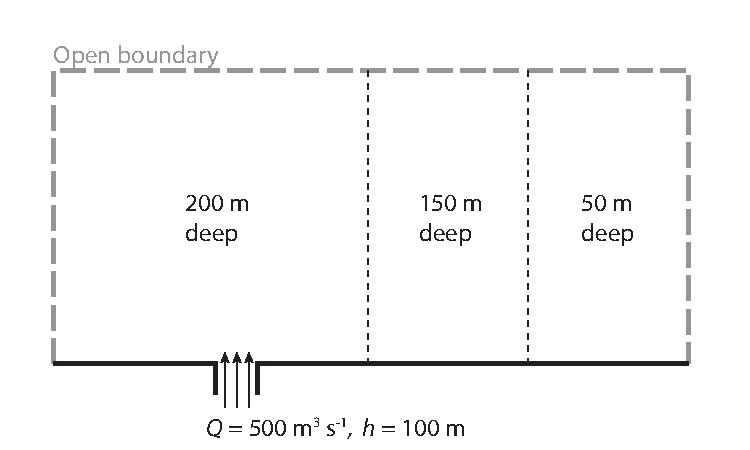
\includegraphics[width=2.9in]{ideal1.pdf}\hfill
    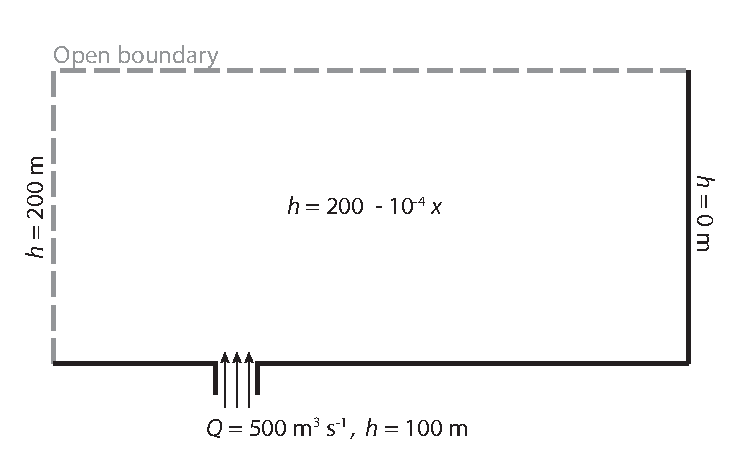
\includegraphics[width=2.9in]{ideal2.pdf}
  % \caption{The bathymetry and geometry of the two idealized coastal domains are shown.}
  \label{fig:ideal}
\end{figure}

\clearpage
\section{Comparison of linear adjustment and non-linear jet solutions}
\label{prob:step_wall_adjustment}

Imagine an initial condition with a step in sea surface elevation perpendicular to a coastline in a flat, semi-infinite coastal ocean.  When the gate maintaining this step is released, the flow will adjust such that the geostrophic flow is directed toward the coast.  Now, consider two models that might describe how this adjustment might evolve.

The first model is a linear model.  Combining the geostrophic flow of the step adjustment problem, with the Kelvin wave solution along the coast, it is clear by considering the elevation far from the coast and initial step, and considering the sea surface elevation along the coast set by the propagating Kelvin wave that the flow will be such that the coastward transport is balanced by an equivalent transport carried by a coastal current directed downcoast.

Now, consider the non-linear jet impinging on a coastal wall model.  If momentum flux is to be conserved, half of the momentum must be carried upcoast, the other half downcoast.

Compare and contrast these two views of coastal adjustment.  Can these two views be reconciled?  Why are they different?  In what ways, if any, are the solutions similar?

\begin{figure}[h]
    \centering
    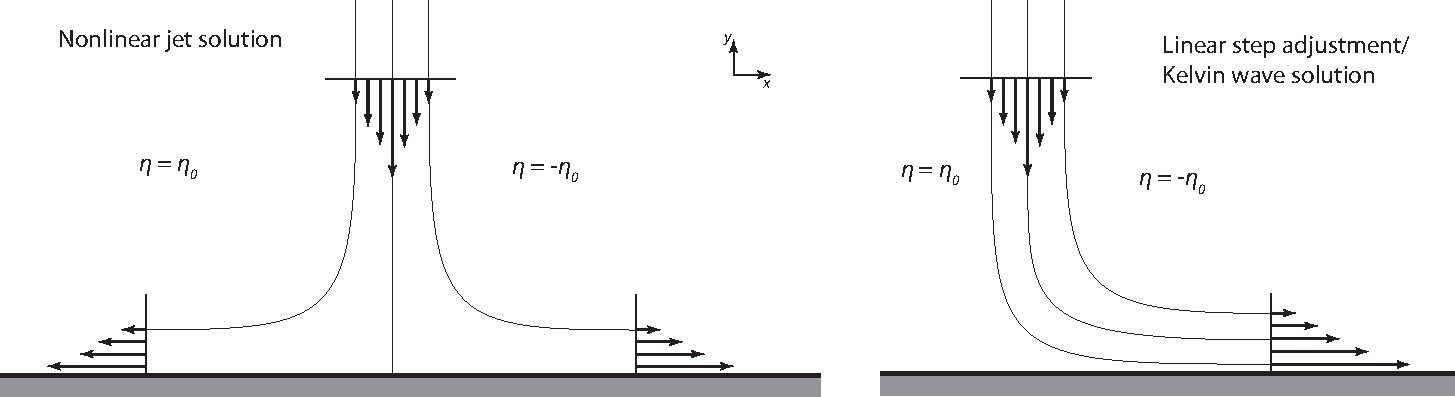
\includegraphics[width=6.5in]{kelvin-vs-jet_adjustment}
    \caption{To conceptual solutions to the adjustment problem of an initial step in sea surface perpendicular to a coastline.}
    \label{fig:kelvin-vs-jet_adjustment}
\end{figure}

\clearpage

\section{Wind-forced Kelvin wave over a uniformly sloping bottom}
\label{prob:wind_forced_kelvin_wave}

Consider the equations used to derive the wind-forced Kelvin wave; again, we will ignore cross-shore wind stress and along-shore variations in forcing.  Instead of a flat bottom, we will assume a linearly sloping bottom, $h = \alpha y$.
\begin{align}
\frac{\partial u}{\partial t} - fv &=  \frac{X}{\alpha y} \\
    f u &= -g\frac{\partial \eta}{\partial y} \\
    \alpha y \frac{\partial v}{\partial y} + \alpha v + \frac{\partial \eta}{\partial t} &= 0.
\end{align}

Some ideas:  It may be useful to assume a periodic solution, so that $\partial/\partial t = i \omega$.  Solutions are some kind of Bessel function.  The singularity at the coast is a problem.  How could you use the idea of the coastal boundary layer to fix this -- can this idea be used to relocate the coastal boundary condition?

\section{Wind-forced Kelvin wave with bottom friction} 
\label{prob:wind_forced_kelvin_wave_friction}

Consider the equations used to derive the wind-forced Kelvin wave, but this time with the inclusion of bottom friction.  Again, we will ignore cross-shore wind stress and along-shore variations in forcing.
\begin{align}
\frac{\partial u}{\partial t} - fv &=  \frac{X}{H} - \frac{r u}{H} \\
    f u &= -g\frac{\partial \eta}{\partial y}  \\
    \alpha y \frac{\partial v}{\partial y} + \alpha v + \frac{\partial \eta}{\partial t} &= 0. 
\end{align}

Some ideas:  Again, it may be useful to assume a periodic solution, so that $\partial/\partial t = i \omega$.  How does the cross-shore structure function change?  What is the response of the along-shore current at the coast to an step function in wind?  Is it possible to obtain a steady response at the coast for steady wind?  What about the solution offshore?

\clearpage
\section{Non-rotating waves in a stratified flow.}
\label{prob:stratified_waves}

Consider an infinitely deep, stratified fluid, bounded below by a moving,
corrugated bottom
\begin{equation}
h(x,t) = h_0 sin (k x - \omega t) = h_0 sin (k (x - U t)).
\end{equation}
We will break the density field into three components, such that
\begin{equation}
\rho = \rho_0 + \bar{\rho}(z) + \rho'(x,y,z,t)
\end{equation}
where each term on the right hand side is very much smaller than its
neighbor to the left (\emph{i.e.}, $\rho_0 \gg \bar{\rho} \gg \rho'$).  Only
$\rho'$ will be considered to be unknown.  The mean vertical
stratification, $\bar{\rho}$, is considered given.  The govorning equations for this system will be
\begin{align}
u_t &= -\frac{p_x}{\rho_0} \\
w_t &= -\frac{p_z}{\rho_0} - \frac{g \rho'}{\rho_0} \\
u_x + w_z &= 0 \\
\rho'_t + w \bar{\rho}_z &= 0
\end{align}
where we are negleting variations (and flow) in the $y$-direction.

\begin{enumerate}
\item Discuss the governing equations.  What physics have been included?
What assumptions have been made?   Describe each equation.
\item Assume a solution of the form \[\phi = \phi_0 e^{i(k x + n z -\omega
t}\] where $\phi$ is any of the dependent variables $u$, $v$, $w$, $p$, or
$\rho'$.  Derive an equation relating $n$ to the other wave properties,
showing that
\begin{equation}
n^2 = \frac{N^2 k^2}{\omega^2} - k^2.
\end{equation}
where $N^2 \equiv -g \bar{\rho}_z / \rho_0$.  You may consider using a
symbolic math solver for this problem.
\item Discuss the $n$ equation.  In particular, what happens when $n$ is
imaginary?  
\item Use the bottom boundary condition to solve first for $w$, then the
other dependent variables.  Plot your solution for two representative
cases: one with real $n$, one with imaginary $n$.
\end{enumerate}




\clearpage 

\bibliographystyle{newapa}
\bibliography{/Users/rob/Dropbox/Documents/hetland}

\clearpage

\printindex

\end{document}

